\documentclass[twocolumn,useAMS,usenatbib]{mn2e}
\usepackage{natbib}
\usepackage{amsmath}
%\usepackage{amssymb}
\usepackage{latexsym}
\usepackage{epsfig,graphicx}
\usepackage{subfig}
\usepackage{float}
\usepackage{color}
\usepackage{hyperref}
\graphicspath{{Figures/}}
\topmargin-1cm

% For correct printing on US Letter, while still working on A4
\topmargin-1cm

\newcommand{\rachel}[1]{{\textcolor{red}{#1}}}
%\newcommand{\rachel}[1]{}
\newcommand{\arun}[1]{{\textcolor{blue}{#1}}}
%\newcommand{\arun}[1]{}
\newcommand{\claire}[1]{{\textcolor{green}{#1}}}
\def\a{\alpha}
\def\reff@jnl#1{{\rm#1\/}}

\def\aj{\reff@jnl{AJ}}                  % Astronomical Journal
\def\araa{\reff@jnl{ARA\&A}}            % Annual Review of Astron and Astrophys
\def\apj{\reff@jnl{ApJ}}                        % Astrophysical Journal
\def\apjl{\reff@jnl{ApJ}}               % Astrophysical Journal, Letters
\def\apjs{\reff@jnl{ApJS}}              % Astrophysical Journal, Supplement
\def\apss{\reff@jnl{Ap\&SS}}            % Astrophysics and Space Science
\def\aap{\reff@jnl{A\&A}}               % Astronomy and Astrophysics
\def\aapr{\reff@jnl{A\&A~Rev.}}         % Astronomy and Astrophysics Reviews
\def\aaps{\reff@jnl{A\&AS}}             % Astronomy and Astrophysics, Supplement
\def\baas{\reff@jnl{BAAS}}              % Bulletin of the AAS
\def\jrasc{\reff@jnl{JRASC}}            % Journal of the RAS of Canada
\def\memras{\reff@jnl{MmRAS}}           % Memoirs of the RAS
\def\mnras{\reff@jnl{MNRAS}}            % Monthly Notices of the RAS
\def\physrep{\reff@jnl{Phys.Rep.}}
\def\pra{\reff@jnl{Phys.Rev.A}}         % Physical Review A: General Physics
\def\prb{\reff@jnl{Phys.Rev.B}}         % Physical Review B: Solid State
\def\prc{\reff@jnl{Phys.Rev.C}}         % Physical Review C
\def\prd{\reff@jnl{Phys.Rev.D}}         % Physical Review D
\def\prl{\reff@jnl{Phys.Rev.Lett}}      % Physical Review Letters
\def\pasp{\reff@jnl{PASP}}              % Publications of the ASP
\def\pasj{\reff@jnl{PASJ}}              % Publications of the ASJ
\def\skytel{\reff@jnl{S\&T}}            % Sky and Telescope
\def\solphys{\reff@jnl{Solar~Phys.}}    % Solar Physics
\def\sovast{\reff@jnl{Soviet~Ast.}}     % Soviet Astronomy
\def\ssr{\reff@jnl{Space~Sci.Rev.}}     % Space Science Reviews
\def\nat{\reff@jnl{Nature}}             % Nature

\def\sun{\hbox{$\odot$}}
\def\farcs{\hbox{$.\!\!^{\prime\prime}$}}
\newcommand{\hvol}{h^{3}{\mathrm{Mpc}}^{-3}}
\newcommand{\hmpc}{\ensuremath{h^{-1}\mathrm{Mpc}}}
\newcommand{\hkpc}{\ensuremath{h^{-1}\mathrm{kpc}}}
\newcommand{\hMsun}{h^{-1}M_{\odot}}
\newcommand{\Msun}{M_{\odot}}
\newcommand{\kms}{{\,{\rm km}\,{\rm s}^{-1}}}
\newcommand{\Omegam}{\Omega_{m}}
\newcommand{\Omegab}{\Omega_{b}}
\newcommand{\Omegal}{\Omega_{\Lambda}}
\newcommand{\xig}{\xi_{\rm gg}(r)}
\newcommand{\xih}{\xi_{\rm hh}(r)}
\newcommand{\xim}{\xi_{\rm mm}(r)}
\newcommand{\ds}{\ensuremath{\Delta\Sigma}}
\newcommand{\scinv}{\ensuremath{\Sigma_c^{-1}}}
\newcommand{\avgscinv}{\ensuremath{\langle\Sigma_c^{-1}\rangle}}
\newcommand{\hinvk}{$h^{-1}$kpc}
\newcommand{\avgnm}{\ensuremath{\langle N(M)\rangle}}
\newcommand{\fclust}{\ensuremath{f_\mathrm{clust}}}
\newcommand{\fbcg}{\ensuremath{f_\mathrm{BCG}}}

\newcommand{\beq}{\begin{equation}}
\newcommand{\eeq}{\end{equation}}
\newcommand{\beqa}{\begin{eqnarray}}
\newcommand{\eeqa}{\end{eqnarray}}

% upright d in integrals
\newcommand{\rmd}{\mathrm{d}}
\newcommand{\putcite}{\textbf{(CITE)}}
\newcommand{\ic}{\ensuremath{I_\mathrm{C}}}
\newcommand{\pc}{\ensuremath{G_\mathrm{C}}}
\newcommand{\ps}{\ensuremath{G_\mathrm{T}}}
\newcommand{\tic}{\ensuremath{\tilde{I}_\mathrm{C}}}
\newcommand{\tpc}{\ensuremath{\tilde{G}_\mathrm{C}}}
\newcommand{\tps}{\ensuremath{\tilde{G}_\mathrm{T}}}
\newcommand{\tkpd}{\ensuremath{\tilde{T}}}
\newcommand{\ticpd}{\ensuremath{\tilde{P}}}
\newcommand{\ticpdr}{\ensuremath{\tilde{P}^\mathrm{(rot)}}}
\newcommand{\ticpds}{\ensuremath{\tilde{P}^{(\gamma)}}}
\newcommand{\ticpdrs}{\ensuremath{\tilde{P}^{(\mathrm{rot},\gamma)}}}
\newcommand{\tks}{\ensuremath{\tilde{K}_\mathrm{T}}}
\newcommand{\tksr}{\ensuremath{\tilde{K}_\mathrm{T}^\mathrm{(rot)}}}
\newcommand{\tis}{\ensuremath{\tilde{I}^{(\gamma)}_\mathrm{T}}}
\newcommand{\tisr}{\ensuremath{\tilde{I}^{(\mathrm{rot},\gamma)}_\mathrm{T}}}
\newcommand{\is}{\ensuremath{I_\mathrm{T}}}
\newcommand{\isr}{\ensuremath{I_\mathrm{T}^\mathrm{(rot)}}}
\newcommand{\rpix}{\ensuremath{R_\mathrm{pix}}}
\newcommand{\nimg}{\ensuremath{N_\mathrm{img}}}
\newcommand{\nrand}{\ensuremath{N_\mathrm{rand}}}
\newcommand{\nset}{\ensuremath{N_\mathrm{set}}}
\newcommand{\nc}{\ensuremath{N_\mathrm{C}}}
\newcommand{\ns}{\ensuremath{N_\mathrm{S}}}
\newcommand{\nt}{\ensuremath{N_\mathrm{T}}}
\newcommand{\erms}{\ensuremath{e_\mathrm{rms}}}
\newcommand{\etot}{\ensuremath{e_\mathrm{tot}}}
%\newcommand{\newtext}{\emph}
\newcommand{\newtext}{}
\newcommand{\reftext}[1]{\textbf{#1}}
%\newcommand{\arcsec}{\ensuremath{^{\prime\prime}}}

%More new commands by Arun Kannawadi
\newcommand{\mg}{\ensuremath{M_G}}
\newcommand{\mi}{\ensuremath{M_I}}
\newcommand{\sersicn}{S\'{e}rsic $n$ }
\newcommand{\sersic}{S\'{e}rsic }
\newcommand{\btt}{Bulge-to-Total }
\newcommand{\s}{\ensuremath{\mathcal{S}}}
\newcommand{\scinot}[2]{\ensuremath{#1 \times 10^{#2}}} 

\title[WL simulation]{The impact of cosmic variance on simulating weak lensing surveys}

\author[Kannawadi et al.]
{Arun Kannawadi$^1$\thanks{\tt akannawa@andrew.cmu.edu}, 
Rachel Mandelbaum$^1$,
Claire Lackner$^2$, 
\\$^1$McWilliams Center for Cosmology, Carnegie Mellon University, Pittsburgh, PA 15217, USA
\\$^2$Kavli Institute for the Physics and Mathematics of the Universe (WPI), Todai Institutes for Advanced Study,\\ the University of Tokyo, Kashiwa, Japan.
}

\date{\today}

\begin{document}
\bibliographystyle{mn2e2}
\maketitle

\begin{abstract}
According to our current understanding, galaxy shapes and morphologies should depend on various factors such as the local environment. Realistic image simulations for calibration of weak lensing analysis methods that use training samples from the Hubble Space Telescope can therefore be affected by these trends, due to the limited volume of the universe that has been surveyed by Hubble. We will show how redshift slices in a volume-limited subsample of COSMOS can be classified as overdense or underdense (or neither), and how the statistical properties of various morphological parameters such as ellipticity, \sersicn, \btt ratio and color differ in these bins. This study requires a careful distinction between environment effects from large-scale structure, which we do not wish to include in simulations, and general trends in the galaxy population with redshift. We conclude with some guidance for how upcoming surveys can use COSMOS data as the basis for weak lensing simulations without having their conclusions overly affected by cosmic variance.  
\rachel{I have some comments on this abtract, but prefer to do all
  revision of the abstract at the end once the paper is finalized.}
\end{abstract}

\begin{keywords}
 Gravitational lensing: weak --- Cosmology: Large-scale structure of Universe --- Galaxies: evolution.
\end{keywords}


\section{Introduction}
\label{S:intro}

Weak gravitational lensing, the deflection of light by mass, is one of the cleanest ways to study the nature of dark energy by tracking the growth of structure in the Universe as a function of time \citep[e.g.,][]{2001PhR...340..291B,2006astro.ph..9591A,2013PhR...530...87W}.
As light from background sources passes by matter (including dark matter) on its way to us, the apparent shapes of the background galaxies get distorted, and the galaxies get slightly magnified as well.
Because of its sensitivity to dark matter and dark energy, major surveys such as the Hyper Suprime-Cam \citep[HSC;][]{HSC_Overview}, Dark Energy Survey~\citep[DES;][]{DESC}, the KIlo-Degree Survey~\citep[KIDS;][]{KIDS}, the Panoramic Survey Telescope and Rapid Response System~\citep[PanSTARRS;][]{PanSTARRS_2010},
the Large Synoptic Survey Telescope~\citep[LSST;][]{LSST_Book}, Euclid\footnote{\url{http://sci.esa.int/euclid/}, \url{http://www.euclid-ec.org}} \citep{EuclidReport},
%(\rachel{cite http://adsabs.harvard.edu/abs/2011arXiv1110.3193L}),
and Wide-Field Infrared Survey Telescope~\citep[WFIRST;][]{WFIRST_Final}
%(\rachel{for WFIRST, you should actually cite the Spergel et al report that was on the arxiv in the past year, not Green et al})
are planned for the next two decades to gather enormous quantities of weak lensing data that will lead to precise constraints on the growth of structure with time, and therefore cosmological parameters.
%Weak lensing effects need to be removed from the Cosmic Microwave Background (CMB) analysis to understand the initial conditions of the universe.

For the upcoming surveys to achieve their promise, their systematic error budgets must be below their statistical error budgets.
Systematic error budgets for weak lensing surveys typically include
astrophysical effects, such as intrinsic alignments of galaxy shapes
with large scale density fields \citep[e.g.,][]{2014arXiv1407.6990T} and the effect of baryons on the
matter power spectrum \citep[e.g.,][]{2011MNRAS.415.3649V}, as well as observational uncertainties such as
the ability to robustly infer shears from galaxy observed shapes or
photometric redshifts from their observed colors. 
Given the expected sub-per cent errors on upcoming surveys, systematic errors must be reduced from
 their typical level in the current state-of-the-art
 measurements that typically achieve $\sim 5$ per cent statistical
 errors at best
 \citep[e.g.,][]{2010A&A...516A..63S,2013MNRAS.432.2433H,2013ApJ...765...74J,2013MNRAS.432.1544M}.

One method that is commonly used to test for the presence of
systematic errors in the shear estimation process is image simulation,
where we can cleanly test whether our methods of shear estimation
recover the ground truth. This is a valuable test, considering the
numerous sources of additive and multiplicative bias such as a
mismatch between galaxy model assumptions and actual galaxy light
profiles \citep[e.g.,][]{2010MNRAS.404..458V, 2010A&A...510A..75M}, biases due to the effects of pixel noise on the
shear estimates
\citep{2012MNRAS.427.2711K,2012MNRAS.424.2757M,2012MNRAS.425.1951R},
and ellipticity gradients \citep{2010MNRAS.406.2793B}.  These biases
often differ for galaxies with different morphologies (e.g., disks
vs. ellipticals), sizes, $S/N$, and shape \citep{2010MNRAS.405.2044B,2012MNRAS.423.3163K}. 
A general requirement for simulations used to test shear recovery is
that they should be as realistic as possible.
 
 Realistic simulations may use samples based on images from the Hubble
 Space Telescope ({\em HST}).
Software packages like
{\sc GalSim}\footnote{\url{https://github.com/GalSim-developers/GalSim}}
\citep{2014arXiv1407.7676R} can generate images of galaxies from the
{\em HST} as they would appear with an additional lensing shear and
viewed by some lower resolution telescope.  Examples of training samples from the {\em HST} include 
the COSMOS survey \citep[used by the GREAT3 challenge,][]{great3} or the
 Ultra Deep Field \citep[UDF, used by][]{2013ApJ...765...74J}.  These
 two examples serve as the extremes in the {\em HST} samples used as
 the basis for image simulation, with COSMOS being shallower but
representing the current widest contiguous area surveyed by the {\em HST}, and the
 latter being extremely deep but narrow.

For a variety of physical reasons, some of which are still not fully
understood, the shape and morphology of
galaxies depends on their local environment
\citep[e.g.,][]{2014arXiv1402.1172C,2014MNRAS.444.2200D}. 
Hence, local overdensities or underdensities
observed in these {\em HST} fields may (given the small size of the field)
cause the properties of the galaxy population in redshift slices to be
atypical depending on the environment in that slice.  This would have
the undesired consequence of including variation in galaxy properties
due to the COSMOS (or other) survey cosmic variance in the simulated galaxy sample in that redshift slice, rather than
only including ensemble effects that would appear in a large cosmological volume, such as true redshift evolution of
galaxy properties.  Our goal is to quantify the degree to which the
morphology-density correlations in COSMOS cause noticeable changes in
the galaxy populations in narrow redshift slices at a level that could
result in difficulty using the sample to derive redshift-dependent
shear calibrations.   Upcoming surveys will study lensing as a function of
redshift and therefore need to simulate galaxy samples at different
redshifts in order to assess the shear calibration at each redshift.

%The structure of the paper is as follows. In \S\ref{S:data}, we briefly describe the COSMOS catalog that we use for our analysis.
The paper is structured as follows: in Sec.~\ref{S:data}, we describe
the data that we use for this study.  In Sec.~\ref{S:methods}, we
describe our methods for deriving the relevant galaxy properties
like environment, morphology, and shape.  
Using these ingredients, we present our results in Sec.~\ref{S:results}
and discuss their implications in Sec.~\ref{S:summary}.
\section{Data}
\label{S:data}
%In this analysis, we consider the COSMOS sample of galaxies. 
The COSMOS survey \citep{COSMOS_overview, COSMOS_generic, COSMOS_Alexie} is a flux-limited, narrow deep field survey covering a contiguous area of $1.64 \text{ deg}^2$ of sky, with images taken using the Advanced Camera for Surveys (ACS) Wide Field Channel (WFC)
in the Hubble Space Telescope (HST).  We use the COSMOS survey to
define a parent sample of galaxy images to be used for making image
simulations, following the approach taken to this problem in
\cite{2012MNRAS.420.1518M,great3}.

We apply the following set of initial cuts to the COSMOS data, the
first two of which
are motivated and explained in more detail by \cite{COSMOS_Alexie}:
\begin{enumerate}
 \item \texttt{MU\_CLASS=1}: This criterion uses a comparison between
   the peak surface brightness and the background level to achieve a
   robust star/galaxy separation, with galaxies having \texttt{MU\_CLASS=1}. 
 \item \texttt{CLEAN=1}: Objects near bright stars or those containing
   saturated pixels were removed; the rest pass this cut on \texttt{CLEAN}. 
% \item \texttt{GOOD\_ZPHOT\_SOURCE=1}: This cut requires that there be a good photometric redshift, which typically is equivalent to requiring that the galaxy not be located within
%                                       the masked regions of the Subaru $BVIz$ imaging used for photometric redshifts, and that it have a successful match against an object in the Subaru imaging
%                                       \arun{copied from Mandelbaum
%                                         2011.}
 \item \texttt{GOOD\_ZPHOT\_SOURCE =1}: This cut requires that
   photometric redshifts be reliable and good enough to draw
   conclusions about the population (see \citealt{2012MNRAS.420.1518M}
   for details).
\end{enumerate}
%\rachel{The cuts you just gave are really basic or fundamental ones.  Those should go before any discussion of more complicated derived quantities like redshifts, stellar mass, Sersic fits, etc.}

%Precise shape measurements, when compared to ground-based surveys, can be made since the full width half-maximum (FWHM) of the point-spread function (PSF)
%is $0.12''$. 
High resolution images taken through the wide F814W filter (broad
\emph{I}) for all galaxies passing the above cuts were used to create
a collection of postage stamp images for the GREAT3 challenge
\citep{great3}, using the procedure described in
\cite{2012MNRAS.420.1518M}.  Each galaxy postage stamp image has a
corresponding PSF image that can be used by {\sc GalSim} or other
software to remove the effects of the {\em HST} PSF before simulating
the galaxy image as it would appear at lower resolution.

To better characterize the galaxy population, parametric models were
fit to the light profiles of these galaxies.  These were carried out
using the method described in \cite{Claire_Fits}, and include
\sersic{} profile fits and 
2 component bulge $+$ disk fits described in detail in \cite{great3}
and briefly in Sec.~\ref{sub:axisratio} of this work.  

In addition to the ACS/WFC (F814W) imaging, the COSMOS field has also been imaged by Subaru Suprime-Cam, the
Canada-French Hawaii Telescope (CFHT) and KPNO/CTIO, yielding many bands
of imaging data from which to determine high-fidelity photometric
redshifts. 
Photometric redshifts were determined by
\cite{COSMOS_Photoz_30band}. The accuracy of photometric redshifts for
$m_\text{F814W}\le$ 22.5 is $\sigma_{\Delta z} = 0.007(1+z)$; for $m_\text{F814W}\le$ 24, $\sigma_{\Delta z} = 0.012(1+z)$.
The photometric redshift values become noisier beyond $z\sim 1.2$, and
the  fits to the galaxy light profiles are also somewhat noisy once we
go beyond $m_\text{F814W}\sim 23.5$.   
For this reason, we will exclude all galaxies that have F814W
magnitude fainter than 23.5. However, we will use the
$m_\text{F814W}\le 25.2$ sample that was generated for the GREAT3
challenge to estimate the completeness, which is useful when
generating a volume-limited sample (Sec.~\ref{sub:volumelimiting}).
We first use the $z<1$ flux-limited sample to fit parametric redshift
distribution models (Sec.~\ref{sub:overdensities}), and then
restrict ourselves to $z\le1$ sample for all further analysis. 
% ($S/N \sim 50$ {\bf ?} )
% \rachel{Our catalog has the more up-to-date Ilbert et al. photo-$z$,
%   not the older Mobasher ones.  Need to fix citations. Also, we care
%   about the photo-$z$ accuracy beyond 22.5, so it's important to give
%   some information about it to the depth that we actually use.  Finally, I
%   recommend against mentioning the $S/N$ because the calculation is
%   complicated by the correlated noise, so most people use use
%   magnitude instead of $S/N$.}

Stellar mass estimates were obtained~\citep{COSMOS_XRAY} using the
Bayesian code described in~\cite{KEVIN_MSTAR}.  This process involves
constructing a grid of models that vary in age, star formation
history, dust content and metallicity (always assuming a Chabrier IMF;
\citealt{ChabrierIMF}), 
 to which the observed galaxy spectral energy distributions (SEDs) and photometric redshift are compared. At each grid point, the probability that the 
SED fits the model is calculated, and by marginalizing over the nuisance parameters in the grid, the stellar mass probability distribution is obtained. The median of this distribution
is taken as the stellar mass estimate. 
  
%We will analyze how the galaxy morphology and intrinsic shape depends on
%the environment in which they reside.

\section{Methods}
\label{S:methods}

In order to study the variation in the intrinsic ellipticity
distribution and various morphological indicators with the galaxy environment, there are three main steps to be carried out:
\begin{enumerate}
 \item Identify overdense and underdense environments in our survey
   from the redshift distribution of galaxies (Sec.~\ref{sub:overdensities});
 \item volume-limit the sample such that Malmquist bias is minimized
   before comparing galaxies in different redshift slices
   (Sec.~\ref{sub:volumelimiting}); and 
 \item estimate the galaxy axis ratios and other morphological indicators such as  \sersic{} index and bulge-to-total ratios (Sec.~\ref{sub:axisratio}).
\end{enumerate}

In this section we will describe how these steps were carried out.

%\rachel{Here you should put a few introductory sentences about the purpose of this section. Could be something like ``To study the  variation in the intrinsic ellipticity distribution with environment, there are two main steps.  The first is to identify redshift ranges with overdense and underdense environments.  The second is to estimate galaxy axis ratios.  In this section we describe how these two steps were done.''}

\subsection{Finding overdensities}
\label{sub:overdensities}
\begin{figure}
 \centering
  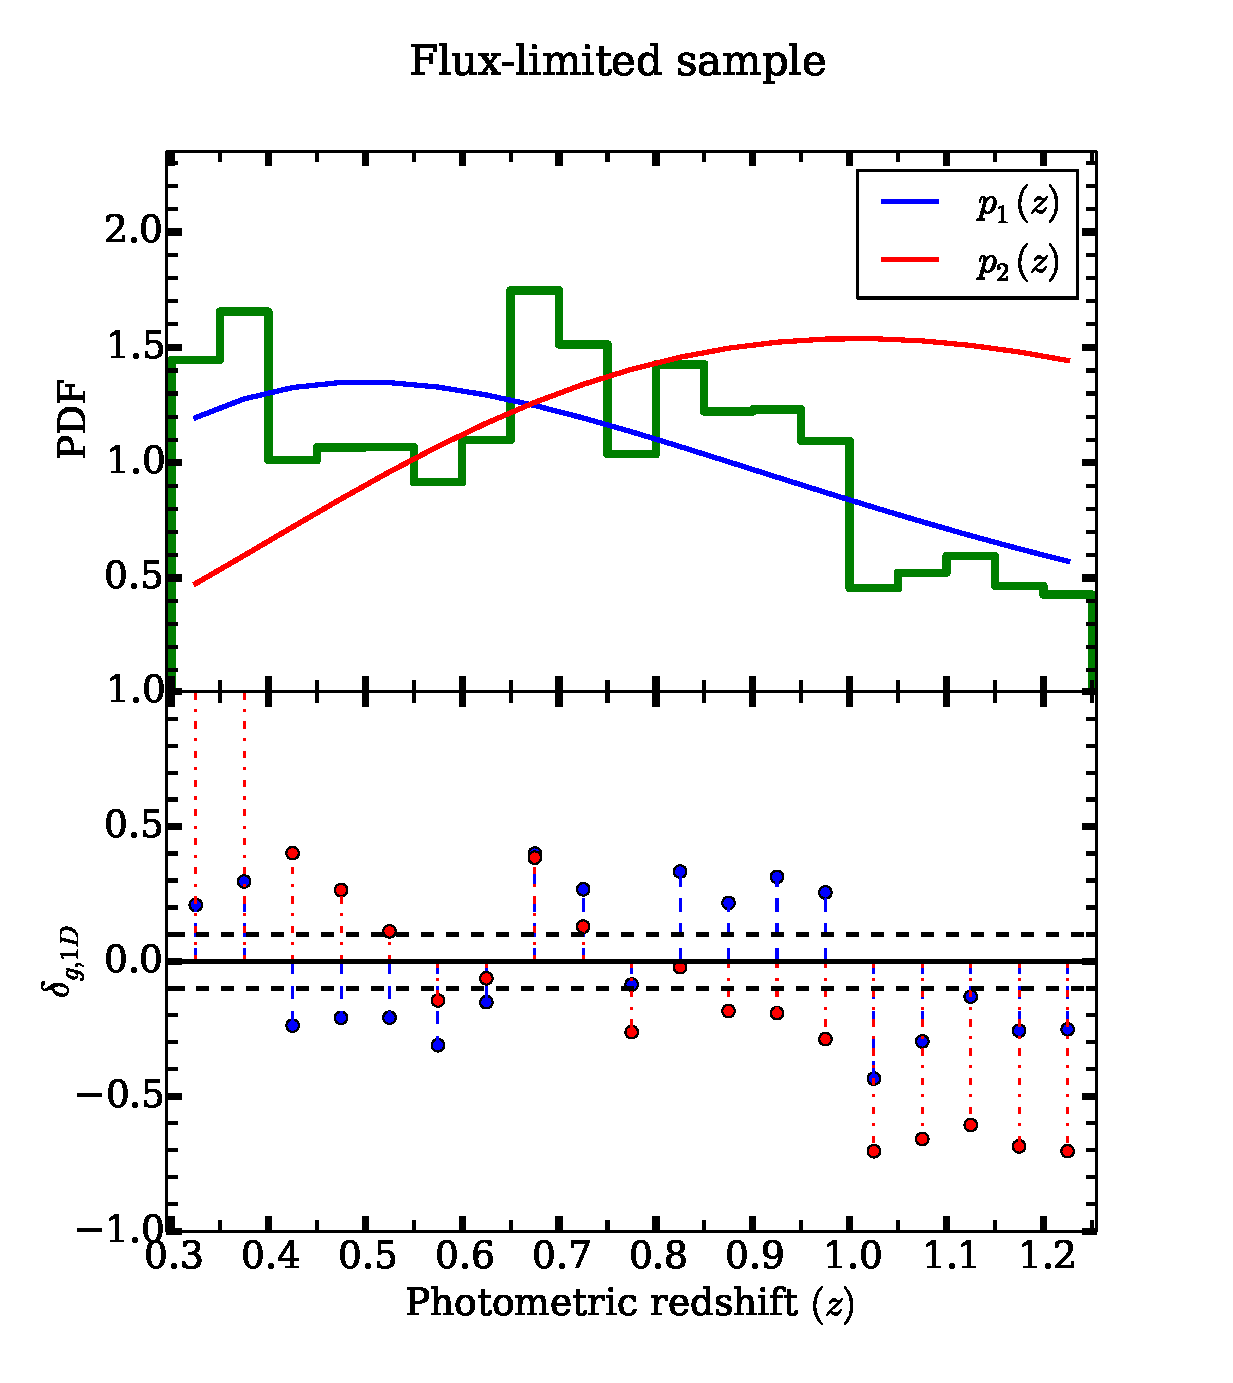
\includegraphics[width=\columnwidth]{redshift_fluxlimited}
  %\caption{\rachel{You show this figure twice.  Why?  The legend needs to say the name of the distribution, not show the functional form.}}
  \caption{Upper panel: Redshift distribution of flux-limited
    ($m_\text{F814W}\le 23.5$) sample with photometric redshift bins that are 0.05 wide. Two analytical functions with best fit parameters are plotted over it.\
           Lower panel: Plot of $(1+\delta_{g,\text{1D}}) =
           N/N_{\text{mod}}$ with each functional form as the model
           for each redshift bin. \arun{Give parameter values. Set
             minor ticks.}
\rachel{Change $x$ axis label to ``Photometric redshift ($z$)''.  Use
  thicker line width for the actual histogram.  Change legend to say
  ``$p_1(z)$ (Eq. 1)'' and ``$p_2(z)$ (Eq. 2)'' rather than giving the
actual equation.  Also, why are two of the horizontal lines in the
bottom panel solid and one dashed?  What decides the style for each
line?  Finally, I think it makes sense to plot $\delta$ rather than $1+\delta$.}}
  \label{fig:redshift_fluxlimited}
\end{figure}

%\rachel{I am a bit confused here.  Our initial strategy was as follows: use all galaxies with $F814W<23.5$ or 25.2 to define a redshift distribution that we fit with one of our functional forms, use that to define overdensities, and then later when we're checking
%  the variation of properties with redshift, we restrict to
%  volume-limited subsamples.  But here you seem to be volume-limiting
%  as the first step, which is not really appropriate. The functional
%  forms that people have derived for surveys are predicated on the
%  assumption that they are flux-limited.  What is the justification
%  for volume-limiting first?  if there is none, then we should not be
%  doing it. And then this section will have 3 subsection: finding
%  overdensities, estimating axis ratios, and volume limiting,
%  where we need to explain the two choices (using $B$-band evolution
%  and using no evolution).}

It is important to keep in mind when considering the environment
estimation that our goal is not to create a full 3D mapping of the
density field within the COSMOS region (a task that was already
addressed by \citealt{Kovac_Density10k} using the zCOSMOS
spectroscopic sample).  Instead, we make a coarse, 1D division of the
COSMOS survey into redshift slices, just as would be done when making
galaxy redshift slices as input to a weak lensing survey simulation.
For each redshift slice, we can then check whether the environment is
overdense or underdense on average.  Our approach will tend to wash
out some real trends from a 3D study, but is appropriate given our
scientific goal of testing effects of the environment on weak lensing
simulations based on the COSMOS survey.

%In a wide-field survey, regions of overdensities are selected  identified by computing 3-dimensional comoving densities. But in narrow field surveys like COSMOS, previous work {\bf cite } have shown
%that regions of overdensities can be identified from a 1-dimensional histogram of redshifts, at least for low redshifts. 
%\rachel{This is not entirely the point.  As we've discussed, the point
%  is that we do not care about 3d densities for this particular science.  Weak lensing simulations
%  will use galaxies selected in 2d slices, and hence we will simply do
 % it that way as well.  But we use the comparison with a 3d analysis
 % as a test of our method.}

%\rachel{I thought we were only going up to $z=0.85$ but here you say $1$?}
%For our sample of galaxies, volume-limited upto $z=1$ by imposing an $M_I$ cut, we fit parametric models to the histogram of photometric redshifts in order to assign values of overdensity. The figures show chi-squared and gamma functions fitted to the histogram \citep{Redshift_modelling}.
For our (flux-limited) sample of galaxies, up to $z=1.0$, we fit
parametric models to the histograms of photometric redshifts in order
to assign values of overdensity.  We choose our bins to be $0.05$ wide
starting from $z=0.3$, where the bin width is selected to be somewhat
larger than the photometric redshift error but narrow enough that we
can still identify rather than averaging over real cosmological
structures.  We neglect the lowest
redshifts which have negligible cosmological volume and where the
galaxy population tends to be intrinsically bright and large enough
that a non-negligible fraction is lost due to the cuts we impose
(Sec.~\ref{S:data}).

The parametric redshift distributions that we use are
\begin{equation}\label{E:pz1}
 p_1(z) \propto z^{a-1}\exp({-bz})
\end{equation}
and 
\begin{equation}\label{E:pz2}
 p_2(z) \propto z^2\exp{\left(-\left(\frac{z}{z_0}\right)^{1.5}\right)},
\end{equation}
the latter of which was first presented by
\cite{Redshift_modelling}. Here $a$, $b$, and
$z_0$ are free parameters that are to be determined.  The
normalization constants depend not only on the parameters but also on
the lower and the upper limit of the redshifts considered, where we
fix the normalization to ensure that the predicted number of galaxies
in the range used ($0.3<z<1$) is equal to the actual number. 
Fig.~\ref{fig:redshift_fluxlimited} shows the photometric redshift
histogram together with the best-fitting parametric distributions.
\rachel{The results for the 2nd redshift distribution do not look that
  great.  Does it help if we go to $z<1.25$?  I thought the photo-$z$
  were okay in that regime, and it's only beyond $1.25$ that they get
  really scary.  We could use up to $1.25$ for determining the
  redshift distribution, even if we're only trying to find
  overdensities for $z<1$.}

The estimated overdensity in a redshift bin is defined by comparing
the observed galaxy counts in the bin with the counts that are
predicted in that bin by one of the models in Eqs.~\eqref{E:pz1}
and~\eqref{E:pz2}:
\begin{equation}
\delta_{g,\text{1D}}=\frac{(N-N_{\text{mod}})}{N_{\text{mod}}},
\end{equation}
where
\begin{equation}
N_\text{mod} = \int_{z_\text{min}}^{z_\text{max}} p(z) \,\mathrm{d}z
\end{equation}
is determined by integrating the redshift distribution within the
limits of that redshift slice. 
%(\rachel{This $\delta$ definition is important, so it should be in an equation environment.})
Note that $\delta_{g,\text{1D}}$ is dependent on our choice of model
redshift distribution, and should have a mean value of $0$ over the
entire redshift range. % If a model and the distribution agree, then $\delta_{g,\text{1D}}=0$ for that model at all the redshifts. 

Our decision criterion for identifying overdense and underdense
redshift slices involves leaving a 10 per cent margin around an
overdensity of zero; i.e., if $\left| \delta_{g,\text{1D}} \right| <
0.1$, that is considered ``neutral'' (neither overdense nor
underdense on average).  We can then label each redshift slice as
either overdense, underdense, or neutral as follows: 
We label a redshift bin as overdense if at least one model gives a
value of $\delta_{g,\text{1D}} > 0.1$ while the other gives
$\delta_{g,\text{1D}} > -0.1$ 
(neutral or overdense), and vice versa for the underdense regions. We
label a redshift bin as neutral if both models give
$\delta_{g,\text{1D}}$ within the neutral region,  
\emph{or} if use of one model redshift distribution results in the
conclusion that the bin is overdense while the over leads to the
conclusion that it is underdense.
We thus identify the regions $z=0.30-0.40$, $0.65-0.75$, and
$0.80-0.85$ as overdense; $z=0.55-0.65$ and $0.75-0.80$ as underdense; and $z=0.40-0.55$ as unclassified. 
%Although, the $z=0.40-0.55$ bin appears to be underdense, for reasons mentioned in \S\ref{sub:volumelimiting}, we will not call them underdense.

We have adopted this purely 1D environment classification for reasons
explained at the beginning of this section. However, as a sanity check
we can compare it with a more rigorous study that includes information
about structure in the plane of the sky.  
 \cite{Kovac_Density10k} used a sample of $\sim$10~000 zCOSMOS
 spectroscopic galaxies with $I_{AB}<22.5$ to reconstruct the three dimensional overdensity field up to $z\sim 1$.
We find that our classification of overdensities and underdensities
agrees with this work, except for our two highest redshift bins.
We believe that this disagreement is due to the errors in our
photometric redshifts, with the overdensity reported by
\cite{Kovac_Density10k} in the $z=0.875-1$ range 
leaking into our $z=0.80-0.85$ slice.


\subsection{Volume limiting}
\label{sub:volumelimiting}
\begin{figure}
  \centering
   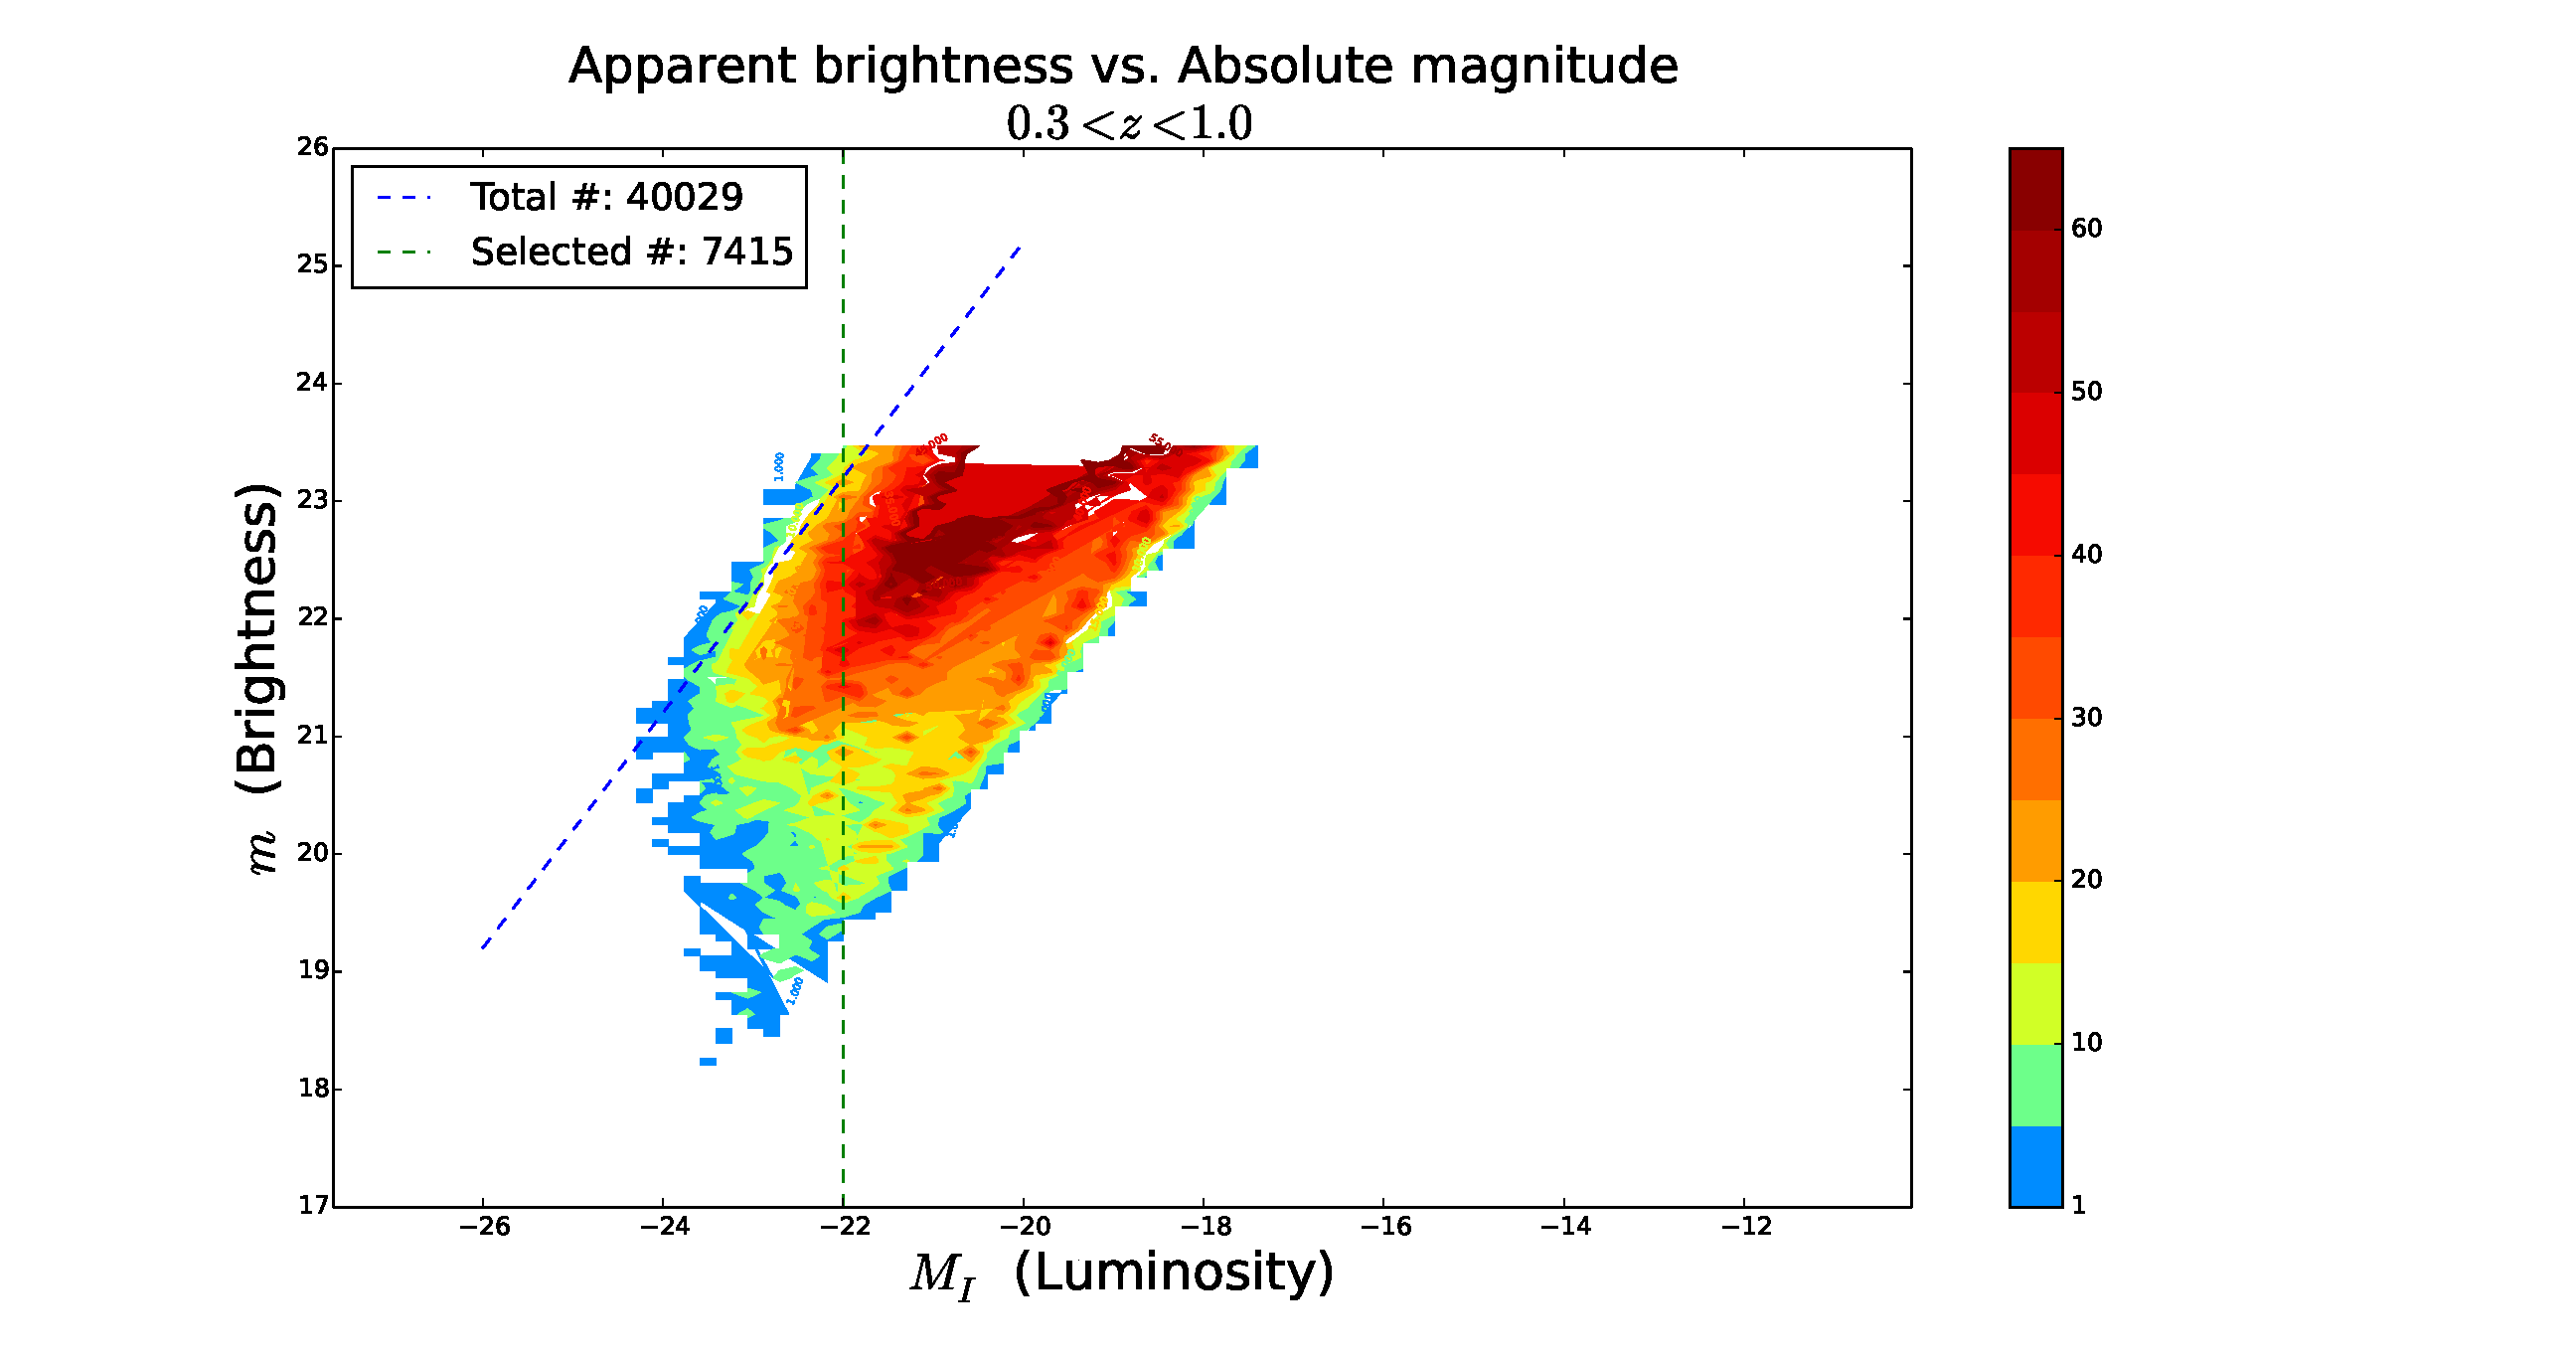
\includegraphics[width=\columnwidth]{hist2d_mag_mi}
   \caption{2-D histogram of galaxies in apparent magnitude ($m_\text{F814W}$) and absolute magnitude ($M_I$) space.}
   \label{fig:2Dhist}
\end{figure}

\begin{figure}
  \centering
   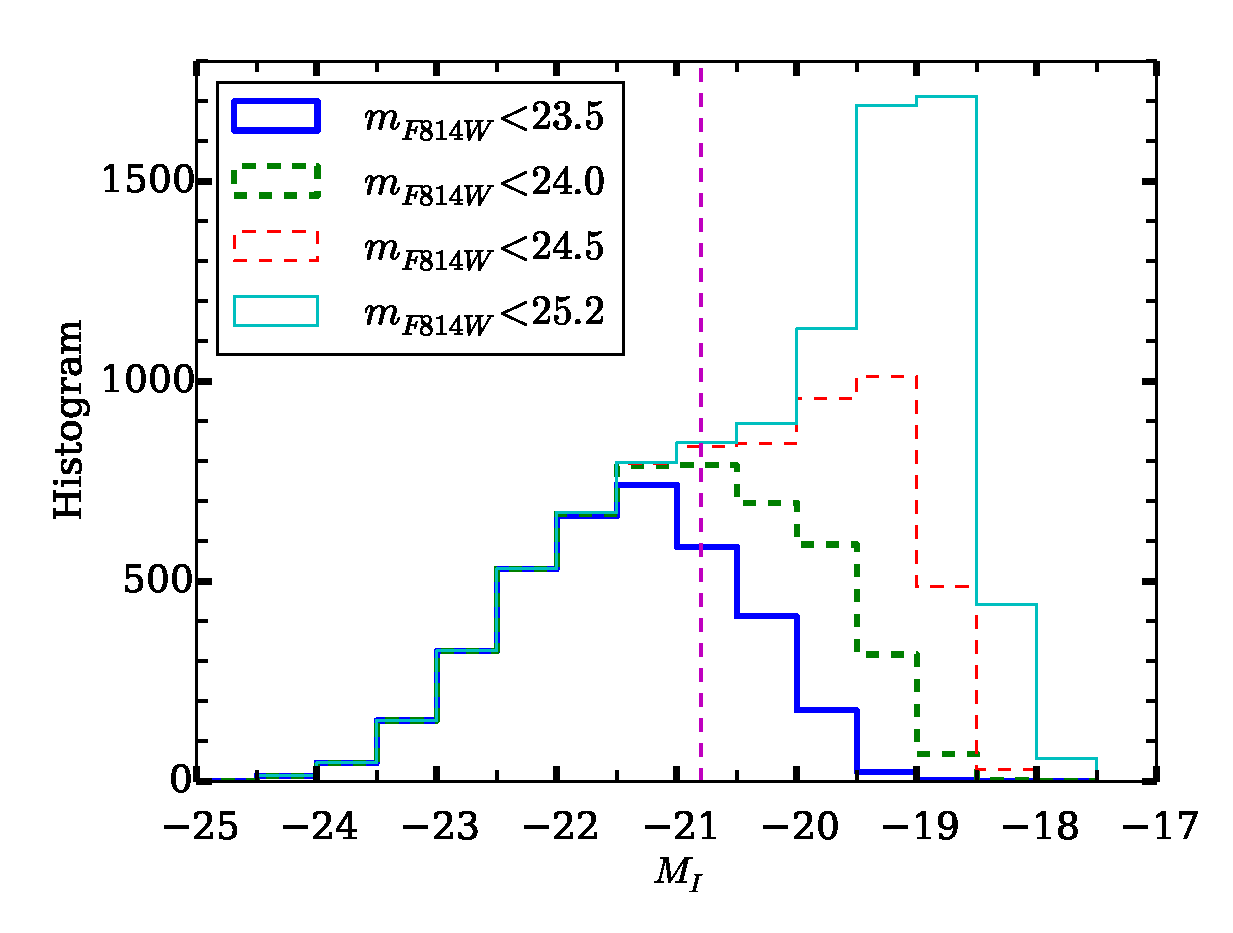
\includegraphics[width=\columnwidth]{MAG_histograms}
   \caption{Distribution of $M_I$ for various flux-limited samples are plotted together. The vertical line corresponds to the luminosity cut of $-20.8$, below which the $m_\text{F814W}<23.5$ sample has 95.3\% of the galaxies in the $m_\text{F814W}<25.2$ sample.}
   \label{fig:MIhist}
 \end{figure}
 
COSMOS is a flux-limited survey and is therefore affected by Malmquist bias, i.e. at higher redshifts, the brighter galaxies are preferentially observed.
Our analysis involves comparing galaxies in different redshift slices to find significant differences in morphology, if any, so with a flux-limited sample, we would be comparing only the bright galaxies at high redshifts with
bright and faint galaxies at low redshifts. For a fair comparison, we must restrict ourselves to bright galaxies at all redshifts and this is acheived by volume-limiting the sample.
%\rachel{Explain why you are doing this.  Before saying {\em how} you
%  generate a volume-limited sample, explain {\em why} you are
%  generating one.}
We generate, using the method below, a volume-limited sample that is complete upto $z=1$ by applying a cut on luminosity such that only galaxies instrinsically brighter than a certain threshold is considered. This threshold is set on  $M_I$, which are $K$-corrected $i^+$-band magnitudes from Subaru or from the PSF-matched CHFT $i^*$-band images.
\rachel{Is it $i$ band, or $I$ band?  Check which one and then be
  self-consistent throughout the text.}\arun{I think they call it
  $I_{814}$, so $I$.}
\rachel{But you are still being ambiguous in sometimes calling it $I$
  and other times F814W.  Pick one.}
\rachel{Actually, is this the catalog entry called ``MI''?  If so, it really is a different band - it's the k-corrected $I$-band data from Suburu or CFHT, so it's appropriate to call it $M_I$ and explain briefly that it's from the Subaru data (but $m_{F814W}$, since MAG\_AUTO is from F814W).}
Since the parent sample contains fainter galaxies, upto $m_\text{F814W}=25.2$, we compare the distribution of the $m_\text{F814W}=23.5$ sample with the samples containing fainter galaxies for high redshift bins, to see where the sample is no longer complete.
% \begin{figure}
%  \centering
%  a) 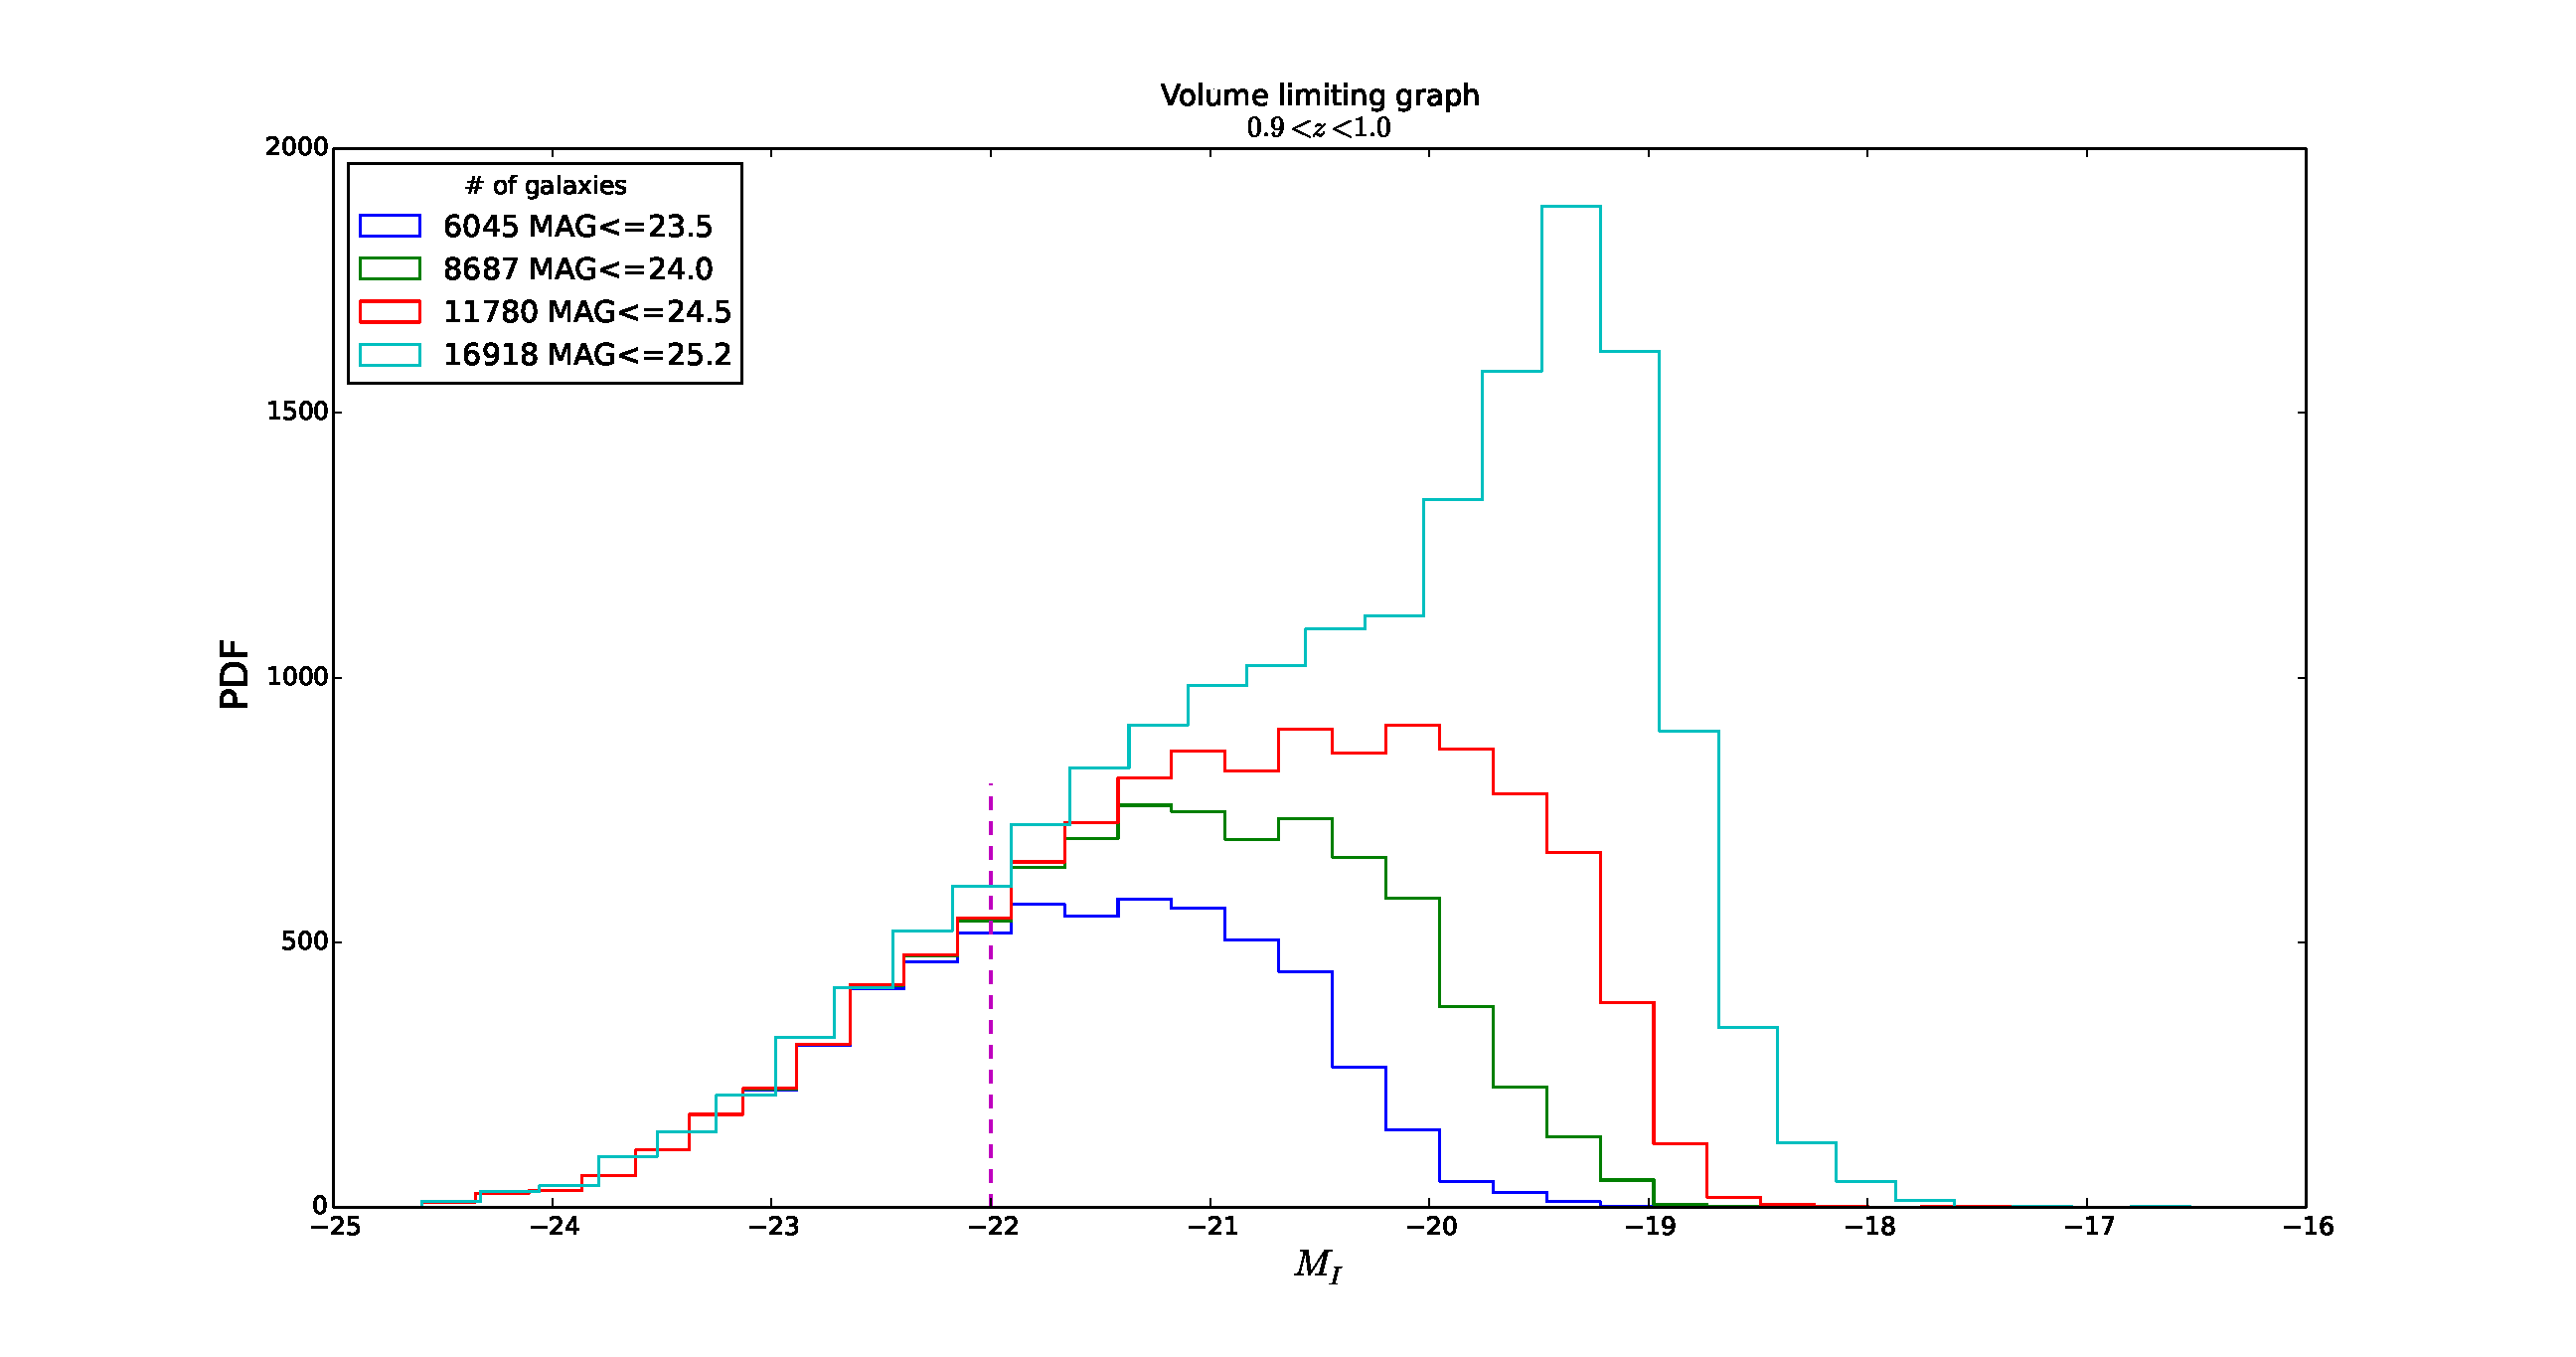
\includegraphics[width=\columnwidth]{volume_limiting_pdf}
%  b) 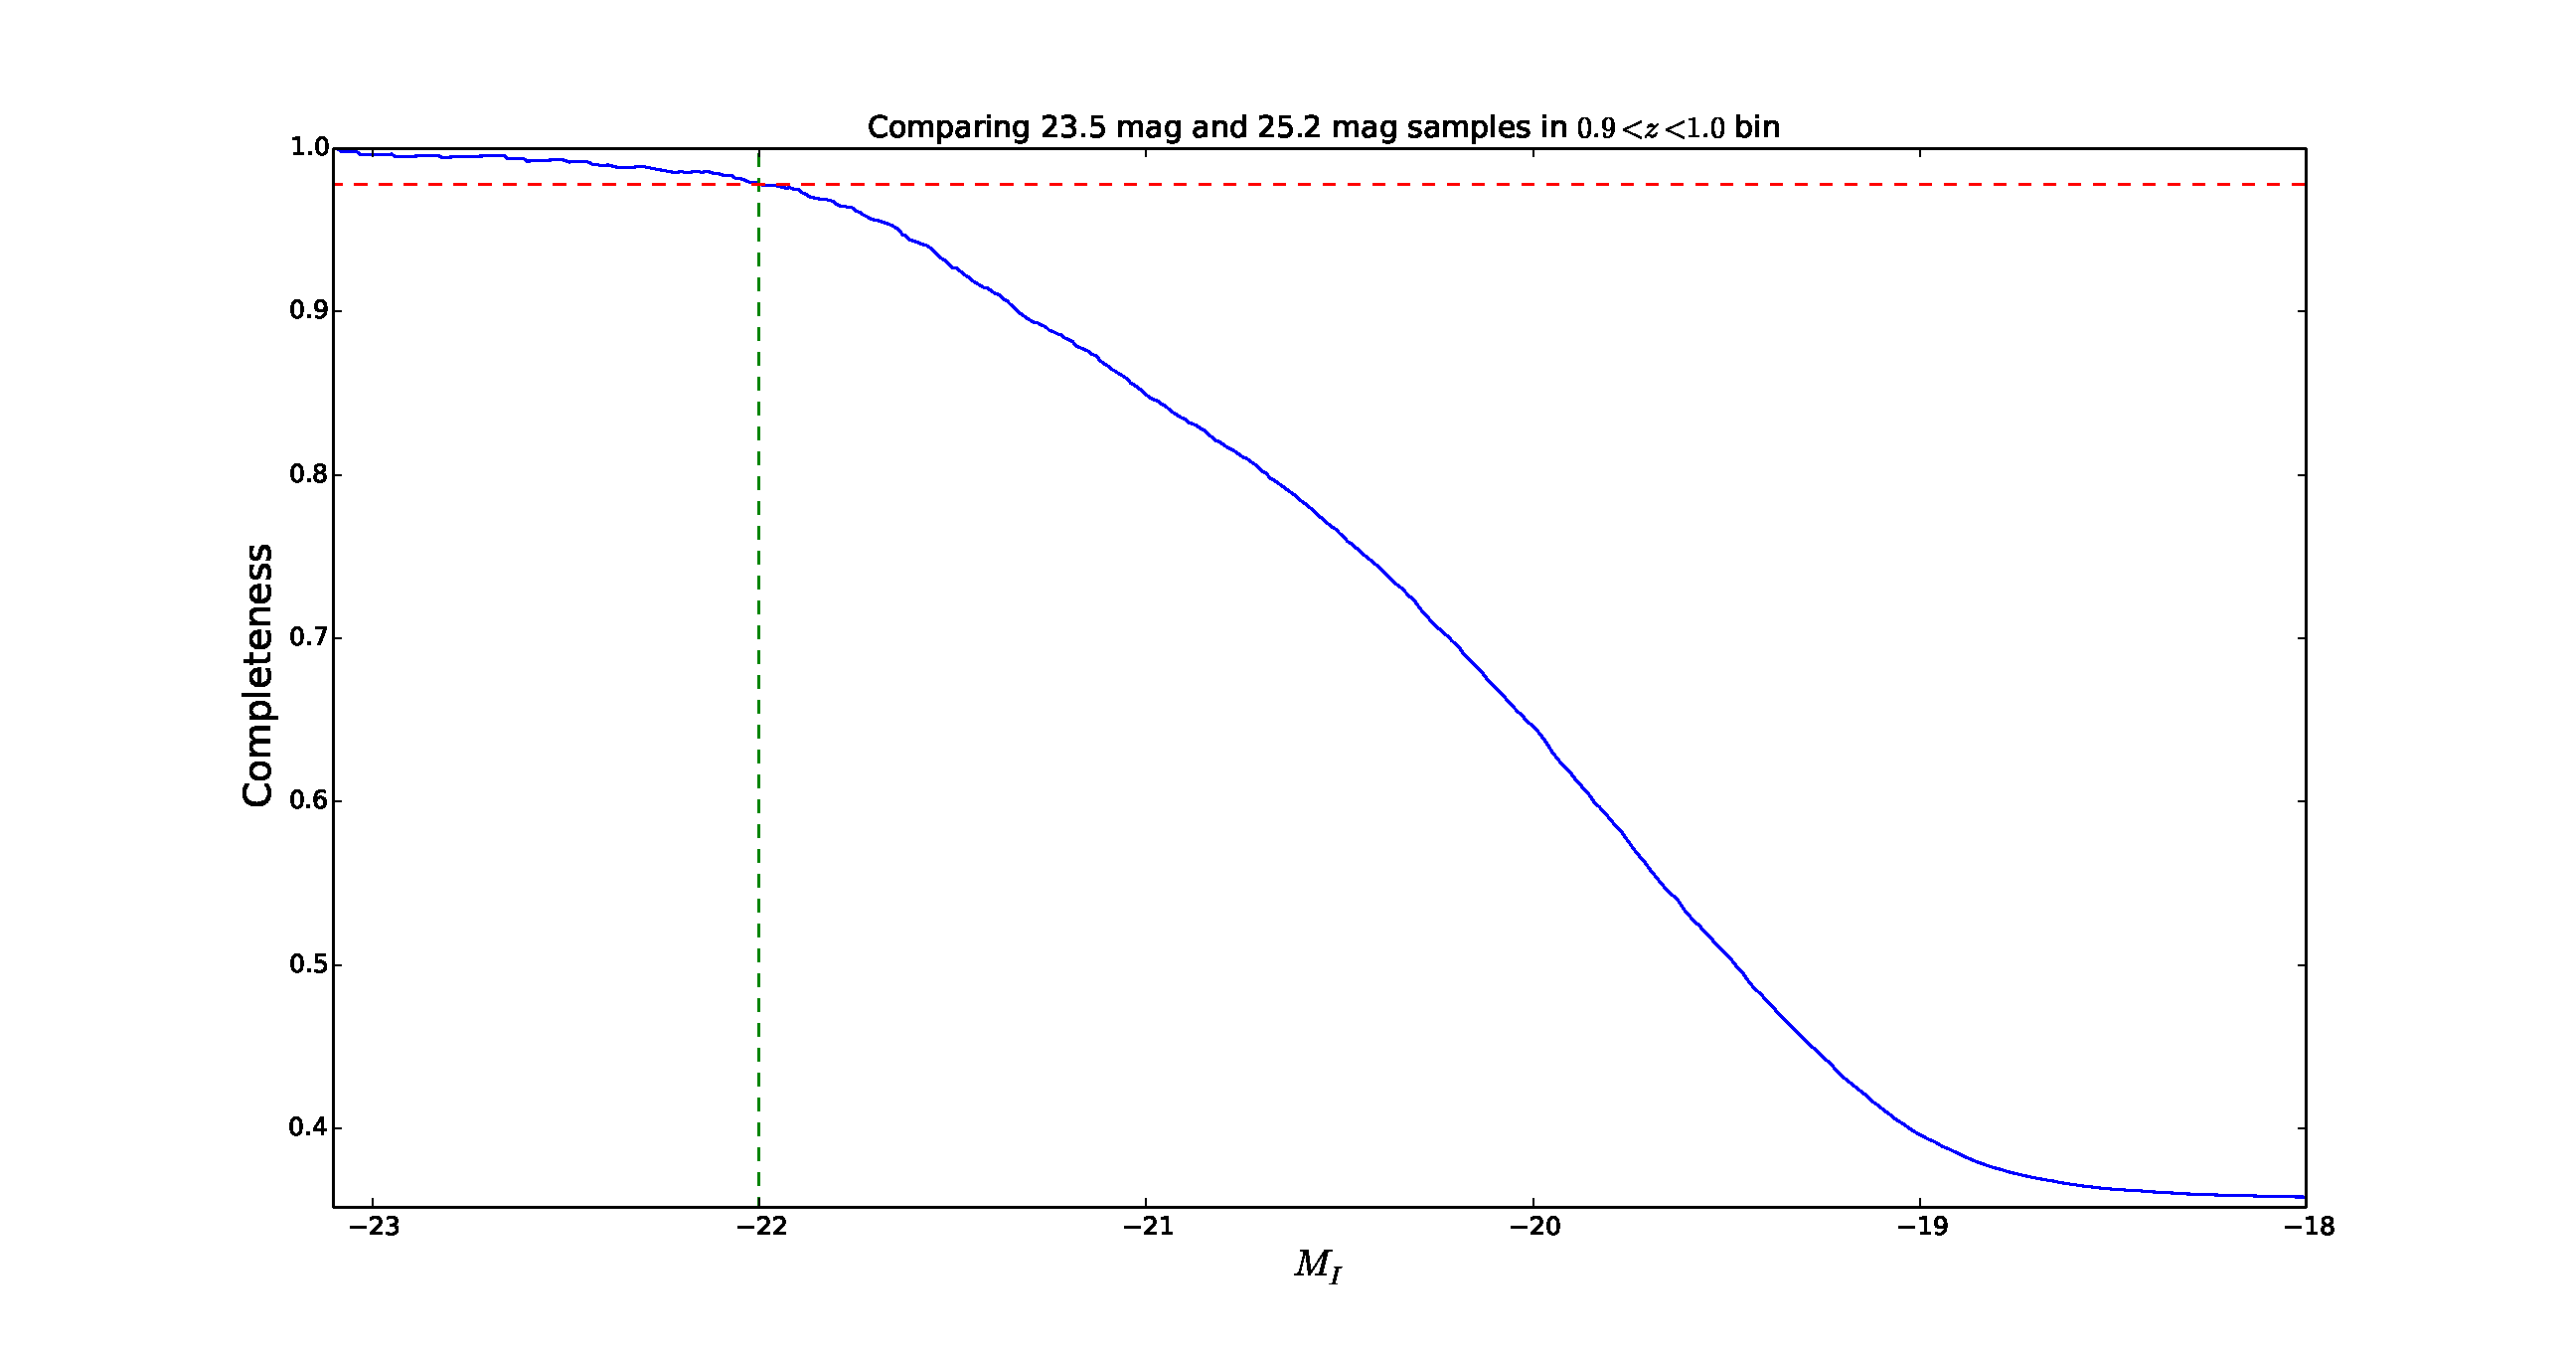
\includegraphics[width=\columnwidth]{volume_limiting_cdf}
%  \label{fig:volume_limiting_dist}
%  \caption{ ... }
% \end{figure}

At $M_I\sim-22.0$, we see the sample is beginning to be biased in the $0.9<z<1.0$ bin due to the flux limit. We obtain 97.84\% completeness in this bin for $M_I$, where completeness is defined as the ratio between the number of galaxies in $m_\text{F814W}\le 23.5$ and in $m_\text{F814W}\le25.2$ samples.
Thus the sample $z\le1$ and $M_I<-22$ is at least 97.84\% complete. Figs.~\ref{fig:2Dhist} \&~\ref{fig:MIhist} show that at $M_I<-22$, we are not affected by flux limit yet. 

%We see that the region between $0.85<z<1.0$ is neither overdense nor underdense according to our model and hence is not going to be considered for further analysis.
The region between $0.85<z<1.0$ is only moderately overdense and we do not seem to have as many underdense regions to compare with. It would rather be advantageous to disregard this region
and redo the volume limiting procedure.
We relax our luminosity cut %to $-20.8$
so that the sample is volume-limited \emph{not} until $z=1$ but until $z=0.85$. 
We choose to impose the cut at $M_I=-20.8$, with 95.3\% completeness in the $0.8 < z \le 0.85$ bin. This increases the sample size significantly, from 7,418 galaxies to 11,169. We call this sample \s$1$.

However, previous studies {\bf cite} have shown that absolute luminosities evolve with redshift. Thus, we must also let the luminosity cut evolve with the redshift. 
There has been no published literature on the LF for the $I$-band, particularly for the COSMOS survey.
We used the published result \citep{Faber2007} for the `rate' of evolution of B-band magnitudes for DEEP2 and COMBO-17 surveys, which is $ \Delta M_B^* \sim -1.23$ mag per unit redshift, for both blue and red galaxies combined together.
Typically, estimates of evolution in K-band are lesser than the estimates of evolution in B and V bands.
Assuming that the evolution is a smooth function of the wavelength, the evolution in I-band is expected to be lesser than that of the B-band. 
Therefore, by considering no evolution and an upper bound on the evolution, we can interpolate what the results would be like for the true $I$-band evolution.

Thus, we construct a second volume-limited sample \s$2$, this time by letting the luminosity cut evolve. Starting from $M_I = -20.8$ for the $0.8<z\le0.85$ bin, we add to it $1.23$ times the difference between the
bincenters to obtain the luminosity cut for the other (lower) redshift bins. At lower redshifts, we allow for fainter galaxies that wouldn't have passed the cut in \s$1$ and hence has more galaxies.

%In our analysis, we imposed the cut on luminosity for all redshift bins while many studies have shown that the characteristic luminosity of galaxies evolve with redshift. 
% The work that is at least close to what we expect is that of
% \cite{Faber2007}, who have studied the evolution of Schechter parameters in the B-band of DEEP2 and COMBO-17 surveys. We consider their reported value of $ \Delta M_B^* \sim -1.23$ per unit redshift, for both blue and red galaxies combined together.
%Although it is the $I$-band that is of relevance to us, we expect the evolution in B-band to be an upper bound on the evolution in I-band. 


%Alternatively, we can impose cuts on stellar mass of the galaxies instead of imposing on the luminosity. 
%If we restrict to galaxies with masses $M$ such that $\log(M/M_\odot) \ge 10.15$, then we have at least {\bf 95.0\% } completeness.
Alternatively, one could get around the problem of considering redshift evolution by imposing cuts on stellar mass instead of absolute luminosity in a particular band. In Fig.~\ref{fig:smf}, we show the stellar mass function (SMF) of our sample for various F814W flux limit.
\cite{Tomczak_SMF} report the SMFs for the ZFOURGE survey, which includes COSMOS. They considered for this work, a single stellar population following a Chabrier IMF \citep{ChabrierIMF}. 
We plot their SMF for \emph{all} galaxies in Fig.~\ref{fig:smf} for
reference. Their SMF is higher than ours since they reach $K_s$-band
$5\sigma$ depth of 24.9. 
As in the case of $M_I$ s, we compare the stellar mass in the $m_\text{F814W}\le23.5$ sample with that of the $m_\text{F814W}\le25.2$ sample. 
The sample $\log(M/M_\odot) > 10.15$ is about 95\% complete in the redshift bin $\left[ 0.75 - 0.85\right]$ and has 10,341 galaxies in total.
Thus, we construct a third volume-limited sample \s$3$ by imposing the stellar mass cut mentioned above. The number of galaxies in redshift slices
are tabulated in Table \ref{table:GalaxyCounts} for all 3 ways of obtaining a volume-limited sample. Stellar-mass limited sample happens to be the smallest one.

\begin{table} 
\centering
\begin{tabular}{|r|c|c|c|c|}
 \hline
 Redshift & Environment & \s$1$ & \s$2$ & \s$3$ \\
 \hline
 0.3-0.4 & Overdense & 1726 & 2505 & 1260 \\
 0.4-0.475 & Neutral & 988 & 1317 & 710 \\
 0.475-0.55 & Neutral & 1410 & 1788 & 902 \\
 0.55-0.65 & Underdense & 1797 & 2193 & 1183 \\
 0.65-0.75 & Overdense & 4059 & 4476 & 2593 \\
 0.75-0.8 & Underdense & 1159 & 1196 & 675 \\
 0.8-0.85 & Overdense & 2428 & 2428 & 1630 \\
 \hline
\end{tabular}
\caption{List of different redshift bins, their environmental classification and the number of galaxies binwise for volume-limited samples constructed in three different ways: using hard luminosity cut (\s$1$), letting the luminosity cut evolve with redshift (\s$2$) and imposing stellar-mass cuts (\s$3$).}
\label{table:GalaxyCounts}
\end{table}

\begin{figure*}
 \centering
 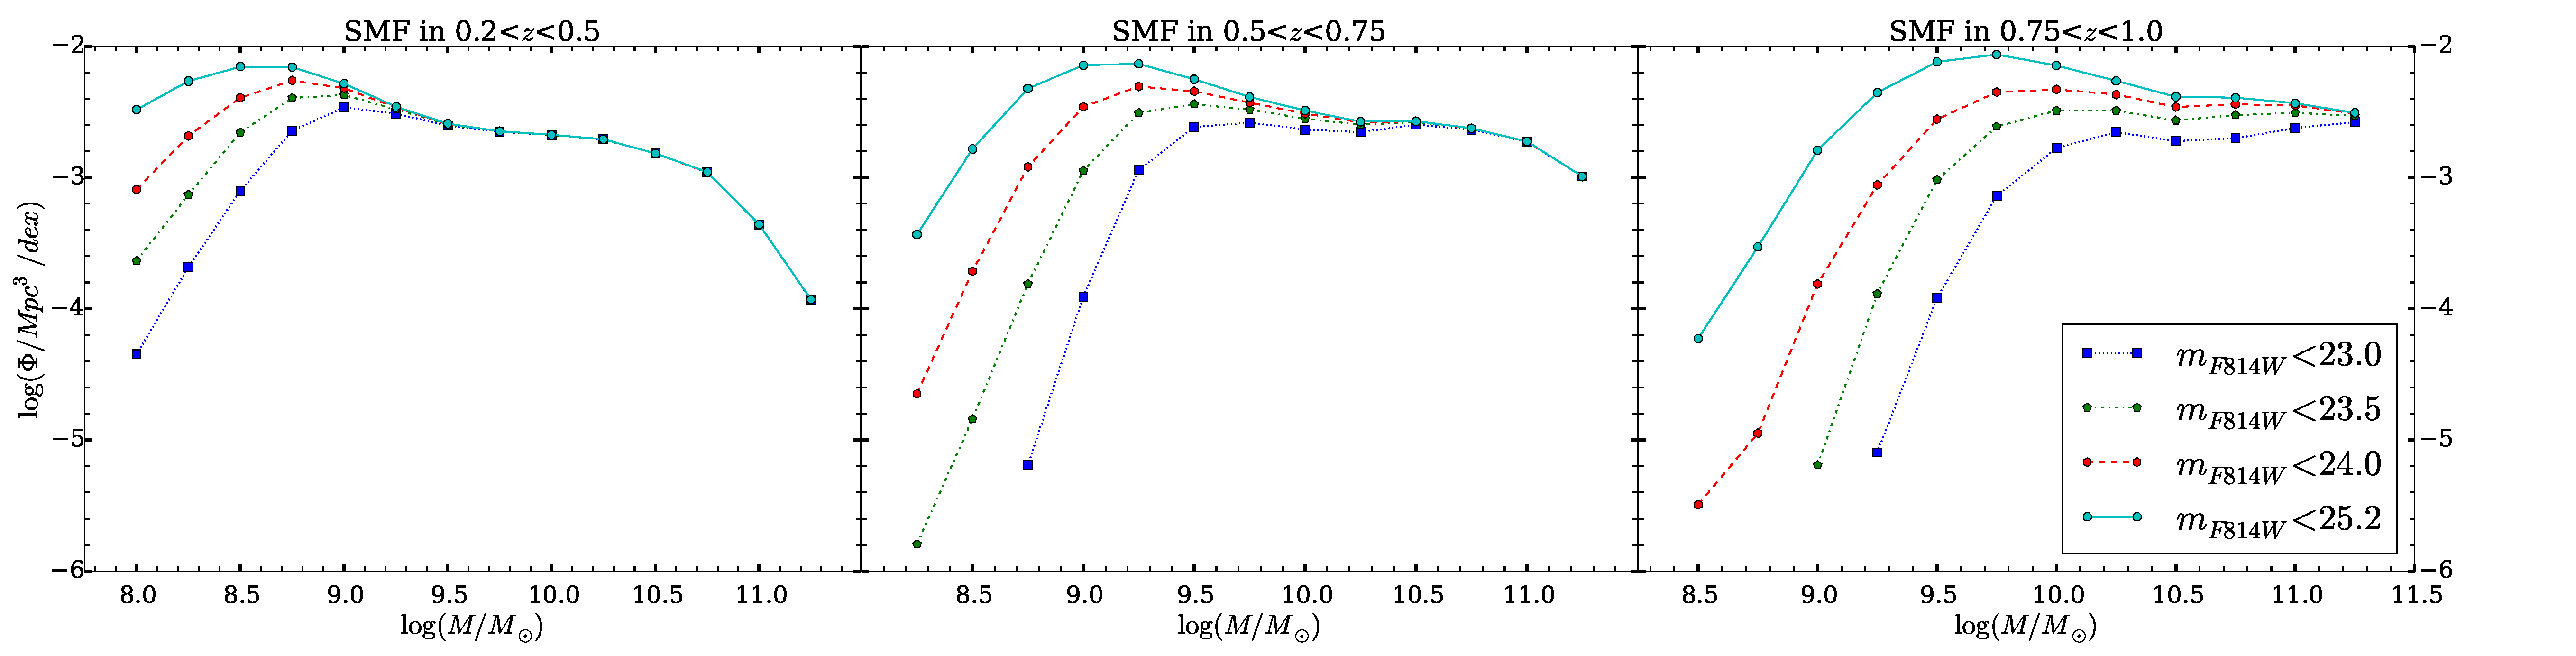
\includegraphics[width=2.4\columnwidth]{SMF}
 \caption{Stellar-mass distribution for various flux-limited samples in three redshift ranges are plotted. Bins have been chosen so as to make the comparison easier with 
          a study of SMF in the same survey \citep{Tomczak_SMF}. At high mass, the distributions are the same for various flux limits indicating that the samples are complete in that mass range. The curves begin to separate at low masses on account of incompleteness, which determines where the mass cutoff should be to volume-limit the sample.}
 \label{fig:smf}
\end{figure*}

There is a minor pitfall with this method. We analyse only those galaxies for which postage stamp images exist.
12\% of galaxies that pass our cuts do not have an associated postage stamp image.
Yet, we use the full $m_\text{F814W}\le23.5$ sample, irrespective of the existence of postage stamps, for identifying overdensities and in the completeness calculation for volume-limiting.
%\rachel{What do you mean we use the full sample  $<23.5$?  For what purpose?  We obviously don't use it for the fits  or shape estimates, so be specific.}
%\arun{Added saying we use the full sample for overdensity calculation and for volume-limiting.}
Postage stamps may not exist because, given the size of the galaxy, the size of the postage stamp we want to draw around it (including enough blank space) intersects with the edge of the CCD.
If all galaxies were the same size, this would be a purely random effect, but in fact bigger galaxies are more likely to get excluded by this cut. 
Typically galaxies that are nearby and intrinsically very bright do not have postage stamps associated with them and this is an effect that is dominant at lower redshifts. 
Our completeness calculation is done at high redshifts and thus we believe that our conclusions are not affected by this bias. 

%Not surprisingly, we see the overdense and underdense regions obtained by the above method have local average number density higher than the global average number density after volume limiting. %Refer to Figure~\ref{fig:comoving_densities}.
%And the environmentally neutral regions fall below or at least lie close to the 10\% margin.
%Refitting the model to our new sample is consistent with the previous assignment of overdensities.

The functional forms for the (flux-limited) redshift distribution that we used in \S\ref{sub:overdensities} are not physically motivated. We fit them again to the  
redshift distribution of a volume-limited sample (\s$1$). Referring to Fig.~\ref{fig:redshift_vollimited}, the values of $\delta_{g,\text{1D}}$ for the $z=0.40-0.55$ bin have increased and are within $\pm 10\%$ of 0. This is the reason why in \S\ref{sub:overdensities} we classified them as neutral as opposed to underdense.
We will see in \S\ref{S:results} that they are more similar to overdense regions as opposed to underdense regions.
The other redshift slices seem to exhibit a consistent behavior. 

\begin{figure}
 \centering
  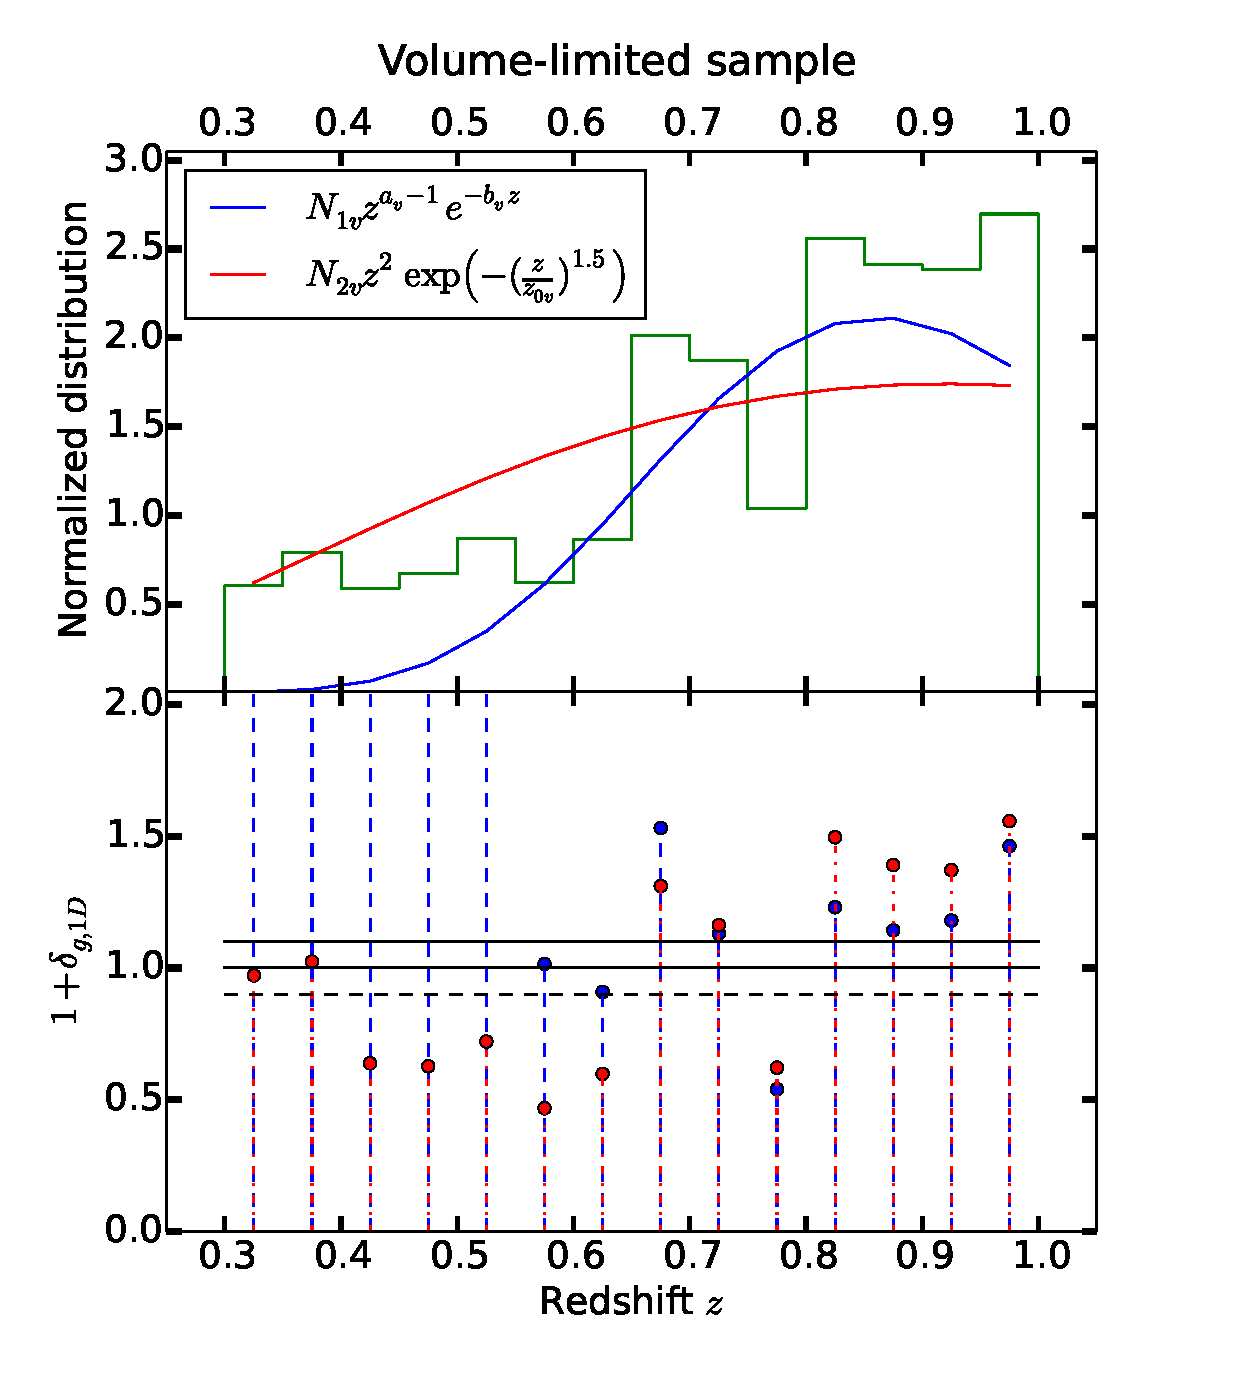
\includegraphics[width=\columnwidth]{redshift_vollimited}
  \caption{Upper panel: Redshift distribution of volume-limited ($M_I <  -20.8$) \s$1$ sample with bins that are 0.05 wide. Two analytical functions with best fit parameters are plotted over it.\
           Lower panel: Plot of $(1+\delta_{g,\text{1D}}) = N/N_{\text{mod}}$ with each functional form as the model for each redshift bin.}
  \label{fig:redshift_vollimited}
\end{figure}

% \begin{figure}
%  \centering
%  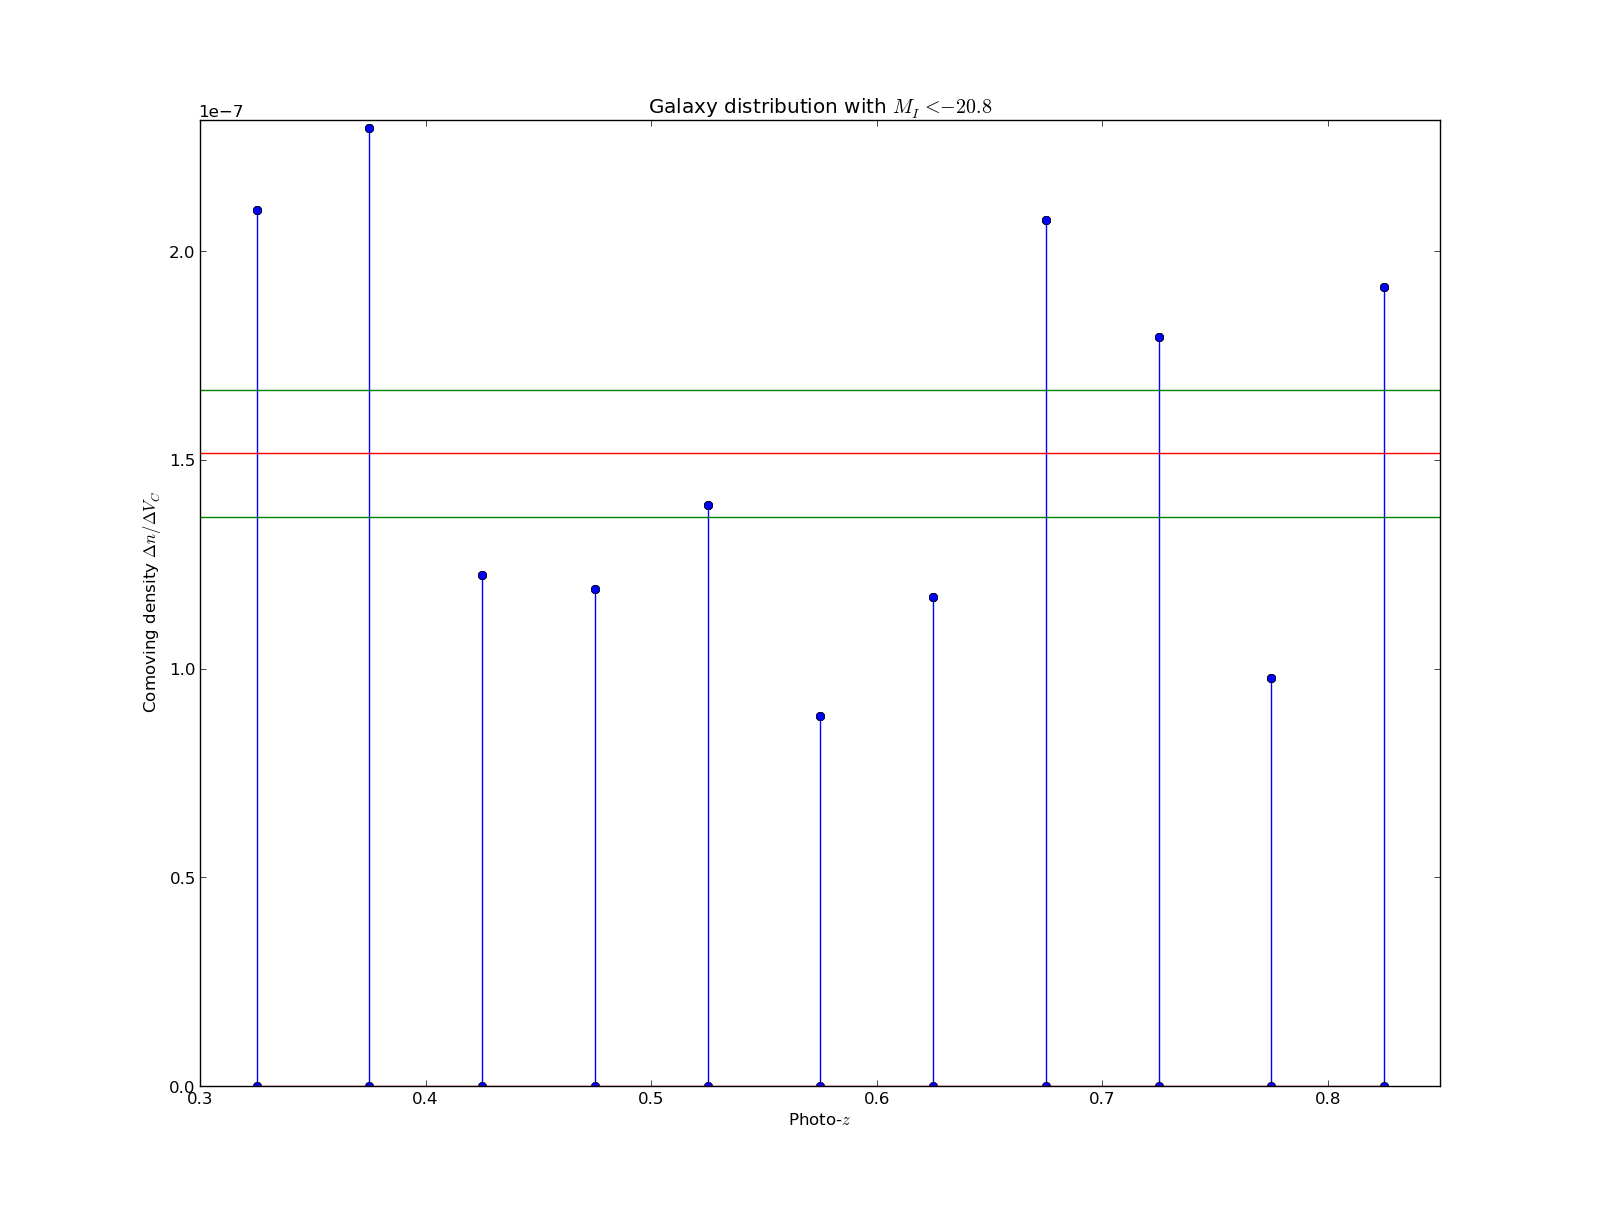
\includegraphics[width=\columnwidth]{../plots_20140219/comoving_densities(2b).png}
%  \label{fig:comoving_densities}
%  \caption{In computing comoving densities, we have chosen the following values for the $\Lambda$CDM parameters: $\Omega_m = 0.3, \Omega_\Lambda = 0.7 \text{ and } \Omega_k = 0$ with the Hubble parameter $h = 0.72$.}
% \end{figure}
  
% \begin{tabular}{c|c|c|c|c|}
%  \hline
%  Redshift & \# of galaxies & Environment \\
%  \hline
%  0.30-0.35 & 726 & 1092 & Overdense \\
%  0.35-0.40 & 1000 1413 & & Overdense \\
%  0.40-0.45 & .. &  \\
%  0.45 - 0.50 & & \\
%  0.50-0.55 & & \\
%  0.55-0.60 & 727 & 905 & Underdense \\
%  0.60-0.65 & 1070 & 1288 & Underdense \\
%  0.65-0.70 & 2089 & 2321 & Overdense \\
%  0.70-0.75 & 1970 & 2155 & Overdense \\
%  0.75-0.80 & 1159 & 1196 & Underdense \\
%  0.80-0.85 & 2428 & 2428 & Overdense \\
%  \hline
% \end{tabular}

In the following section, we will compare and analyze the distribution of properties of the galaxies residing in the overdense regions.

%\arun{Talk more about environments - Nature and nurture?}
%\rachel{What do you have in mind here?}

%\section{Implications/Comparisons}
%\section{Results}
\subsection{Describing galaxy morphology and shape}
\label{sub:axisratio}

% \rachel{As we discussed, you should get rid of the early parts of this
%   regarding second moments, and replace it with a brief description of
%   what shape estimates we use from GalSim (re-Gaussianization).}
% 
% {\bf Should explain in brief Claire's work.} \\

If galaxies have elliptical isophotes, its shape and size could be defined by the axis ratio and the area enclosed by a boundary isophote. However, in real galaxy images,
the boundary may not be well defined and the shape may not be well approximated by an ellipse. More importantly, the effect of smearing due to the point-spread function (PSF) is larger. 
Thus, we are in need of more sophisticated methods to measure the ellipticities.
% Given the surface brightness (intensity) $I(\vec{\theta})$ of a galaxy image at every angular position $\vec{\theta}$,
% we can define the tensor of second brightness moments as
% \begin{equation}
%  Q_{ij} = \frac{\int\rmd^2\theta q_I (\theta_i - \overline{\theta_i})(\theta_j - \overline{\theta_j})}{\int\rmd^2\theta q_I},
% \end{equation}
% where $q_I$ is a suitable chosen kernel and $\overline{\vec{\theta}}$ is the average angular coordinate, weighted by the same kernel function and $i,j\in\lbrace 1,2 \rbrace$ are the components of $\vec{\theta}$.
% It is common to find in literature two kinds of \emph{complex }ellipticities that quantify the shape of the galaxies - $\chi$ and $\epsilon$ defined as
% \begin{align}
%  \chi &= \frac{Q_{11}-Q_{12}+2iQ_{12}}{Q_{11}+Q_{22}} \\ \epsilon &= \frac{Q_{11}-Q_{22}+2iQ_{12}}{Q_{11}+Q_{22}+2(Q_{11}Q_{22}-Q_{12})^{1/2}}
% \end{align}
% If the image has elliptical isophotes with axis ratio $q$, then 
% \begin{equation}
%  |\chi| = \frac{1-q^2}{1+q^2}, \;\;\; |\epsilon| = \frac{1-q}{1+q}. 
% \end{equation}
% 
% 
% Conversely, one could compute $\chi$ or $\epsilon$ for a galaxy, and obtain an effective, azimuthally averaged {\bf(?)} axis-ratio $q$. 
% \rachel{No, that isn't possible because of the PSF.  One would have to
%   use a PSF correction scheme.  Recommend removing much of the above discussion.}
% \arun{Should I remove these even if we plan to use the ellipticities from the second moments?} 

One method to estimate the ellipticities is to estimate the axis-ratios by fitting parametric models to each image. The models that we fit to the images are
\begin{enumerate}
 \item a \sersic profile given by the expression 
       \begin{equation} 
    S = \Sigma_{1/2}\exp{\left( -k(R/R_{\text{eff}})^{1/n} -1 \right)},
       \end{equation}
       \item two \sersic component fits: de Vaucoulers bulge $(n=4)$ + exponential disc profile $(n=1)$,
\end{enumerate}
where \begin{align*} R^2 = & ((x-x_0)\cos\Phi+(y-y_0)\sin\Phi)^2  \\ & + ((y-y_0)\cos\Phi-(x-x_0)\sin\Phi)^2/q^2, \end{align*}
$R_{\text{eff}}$ is the half-light radius of the profile, $\Sigma_{1/2}$ is the surface brightness at $R=R_{\text{eff}}$, $(x_0,y_0)$ is the centroid of the image,
$\Phi$ is the profile rotation angle, $n$ is the \sersic index, $k$ is a $n$-dependent normalization factor and $q$ is the axis ratio of the elliptical isophotes.
Thus, the \sersic profile has 7 free parameters. The bulge+disk model has 10 free parameters since the \sersic indices are fixed as 1 and 4
and both the profiles are required to have the same centroid $(x_0,y_0)$. Best-fit parameters were found, by minimizing the weighted
sum of the difference between the image and the PSF-convolved model
using Levenberg-Marquardt minimization, \texttt{mpfit2fun} in IDL \citep{mpfit2fun}. More details about the fit can be found
in \cite{Claire_Fits}.

The quantities that we would use from the single \sersic profile fits are the \sersic index and axis ratio
and from the bulge+disk fits will be the \btt ratio given by ${\Sigma_{1/2}(n=4)}/{\left(\Sigma_{1/2}(n=4)+\Sigma_{1/2}(n=1)\right)}$.
\rachel{I think it would be useful to take the entire sample that we use for science, and show the overall distributions of axis ratio, distortion (one curve for Claire's and one curve for re-Gaussianization), \sersic index, and \btt.  This would be a nearly full-page four panel figure, but I think it's worthwhile to illustrate the nature of the sample.  For example, it will clearly show why we cannot use the distributions of \sersic index and \btt, because of the hard cutoffs.}

An alternative method involves correcting the observed image for the PSF and computing the covariances from which the ellipticity of the galaxy can be obtained.
The PSF correction scheme used on the observed images is that of `re-Gaussianization' method described in \S 2.4 of \cite{HS03} (hereafter HS03).
This method models the true PSF $g({\bf x})$ as a Gaussian $G({\bf x})$ and the residual $\epsilon({\bf x}) = g({\bf x}) - G({\bf x})$ is assumed to be small. Thus, the Gaussian-convolved
intrinsic image of $f$, is $I' = G\otimes f = I - \epsilon \otimes f$, where $I$ is the observed image. The crucial idea here is that, when $\epsilon$ is small, we get a reasonably accurate
estimate of $I'$ even if we use an approximate form for $f$. The form assumed for $f$ is that of a Gaussian with covariance $M_f^{(0)} = M_I - M_g$, where $M_I$ and $M_g$ are the adaptive
covariances of the measured object and PSF respectively, described in \S 2.1 of HS03, which is in turn based on \cite{BJ02}. Once we obtain the covariance matrices of the instrinsic image $f$, one can compute the ellipticities 
of the galaxies, which we will refer to as `ellipticities based on moments'.

\section{Results}
\label{S:results}
Having identified the overdense and underdense regions in a volume-limited sample (\S\ref{sub:overdensities}, \S\ref{sub:volumelimiting}), we will now see in this section if the morphological
parameters of the galaxies, listed in \S\ref{sub:axisratio}, have any dependence on the environment that they reside in. We have 3 different ways of volume-limiting our sample
\begin{enumerate}
 \item no redshift evolution of luminosity cut $(\s1)$,
 \item use $B$-band evolution rate for $I$-band luminosities $(\s2)$,
 \item impose stellar mass cuts instead of luminosity $(\s3)$
\end{enumerate}
and we will present our results in each of the 3 cases. 

\subsection{Axis-ratios} 
We can understand the influence of environment on the ellipticities of the galaxies simply by comparing the distribution of the axis ratios for the overdense and underdense samples. 
Then, we proceed to consider the root mean square ellipticity, a statistic that can characterize the shape of the population/sample of galaxies. 
\subsubsection{Comparing distributions}
\begin{figure*}
 \centering
 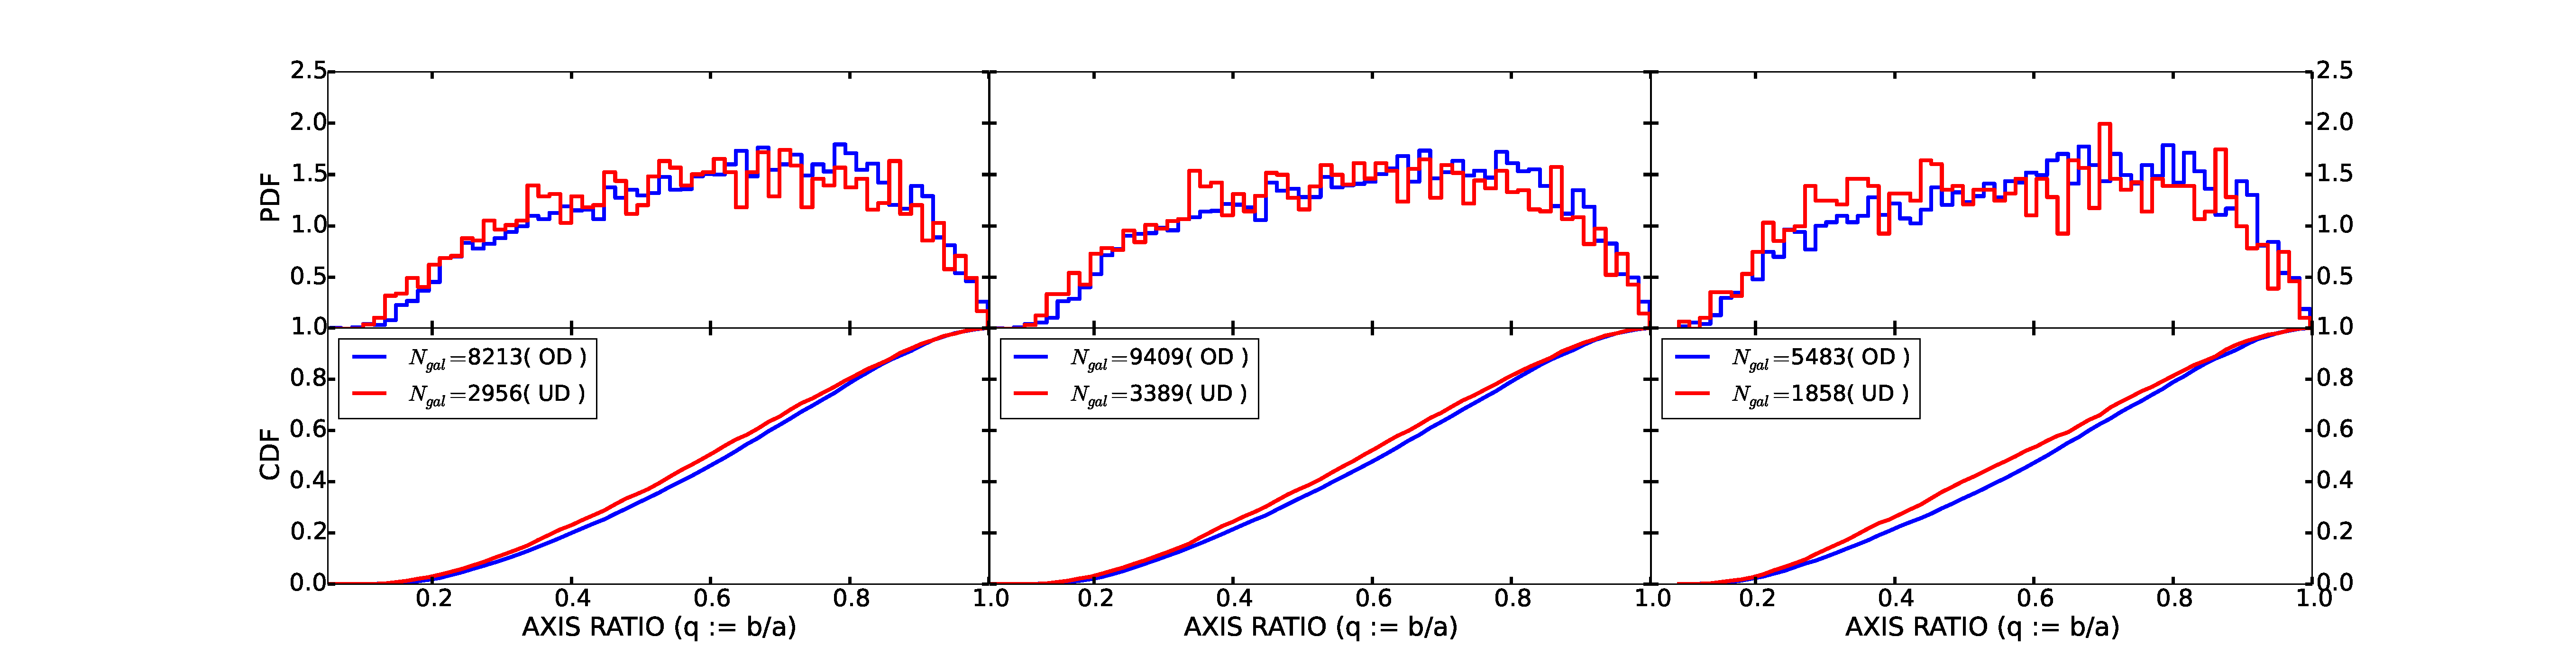
\includegraphics[width=2.3\columnwidth]{axis_ratio_all}
 %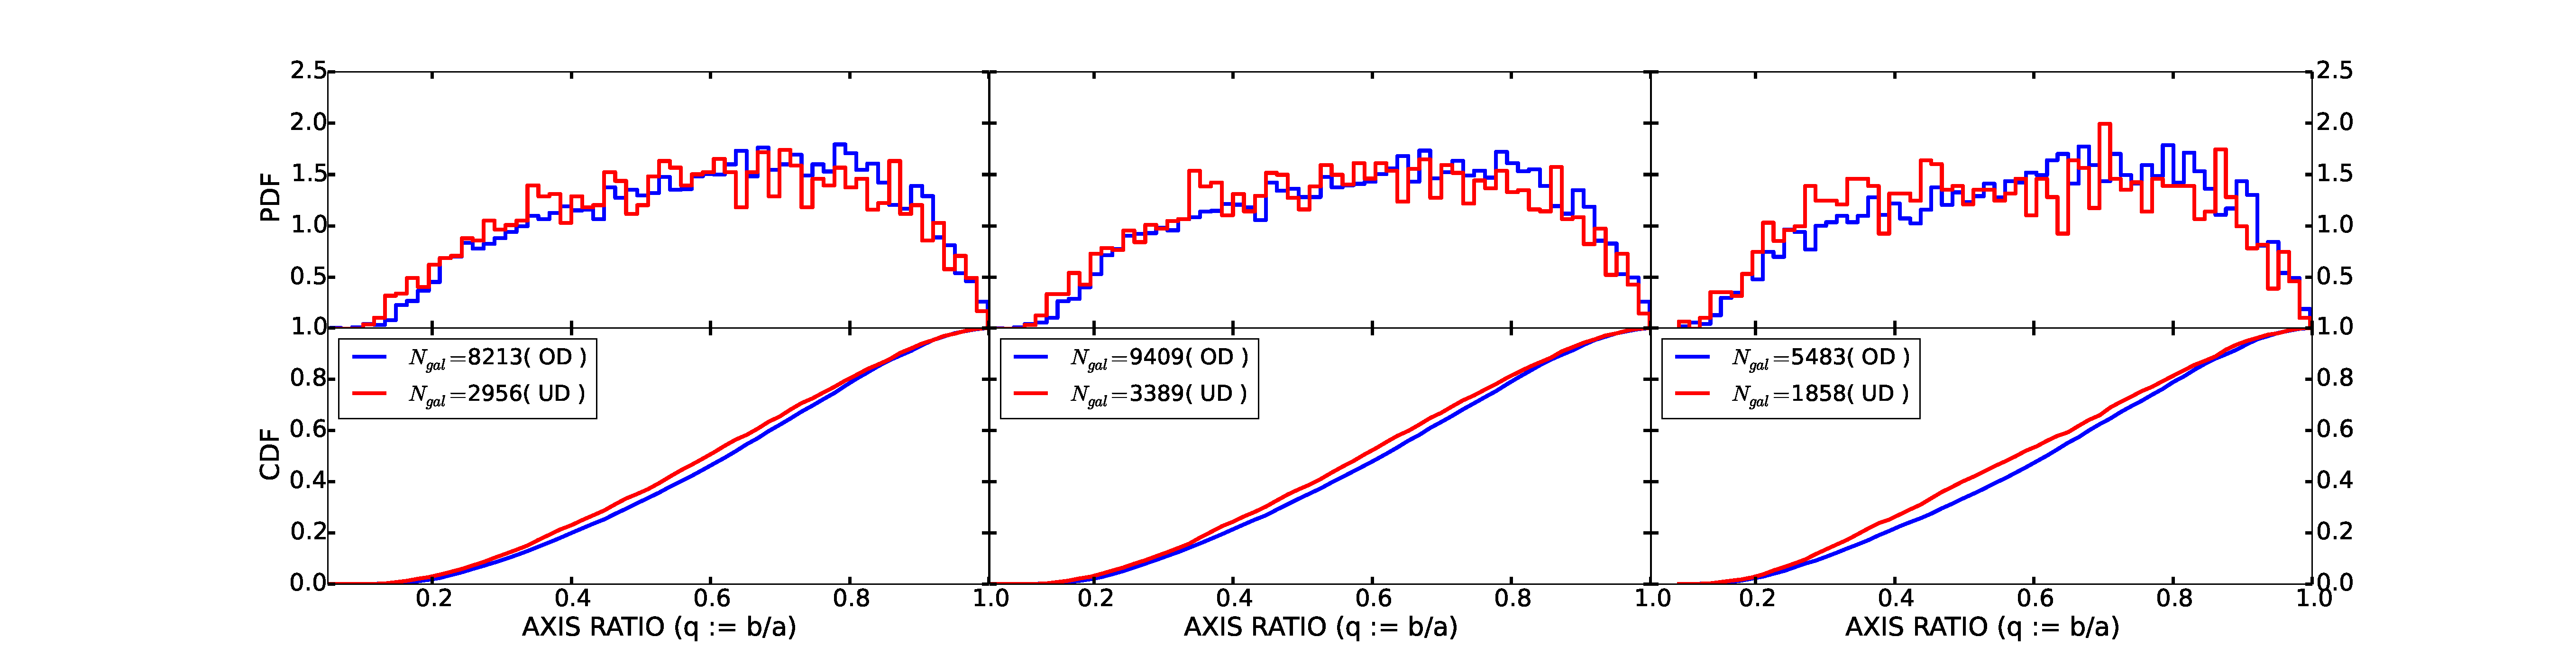
\includegraphics[width=0.66\columnwidth]{axis_ratio_all.eps}
 %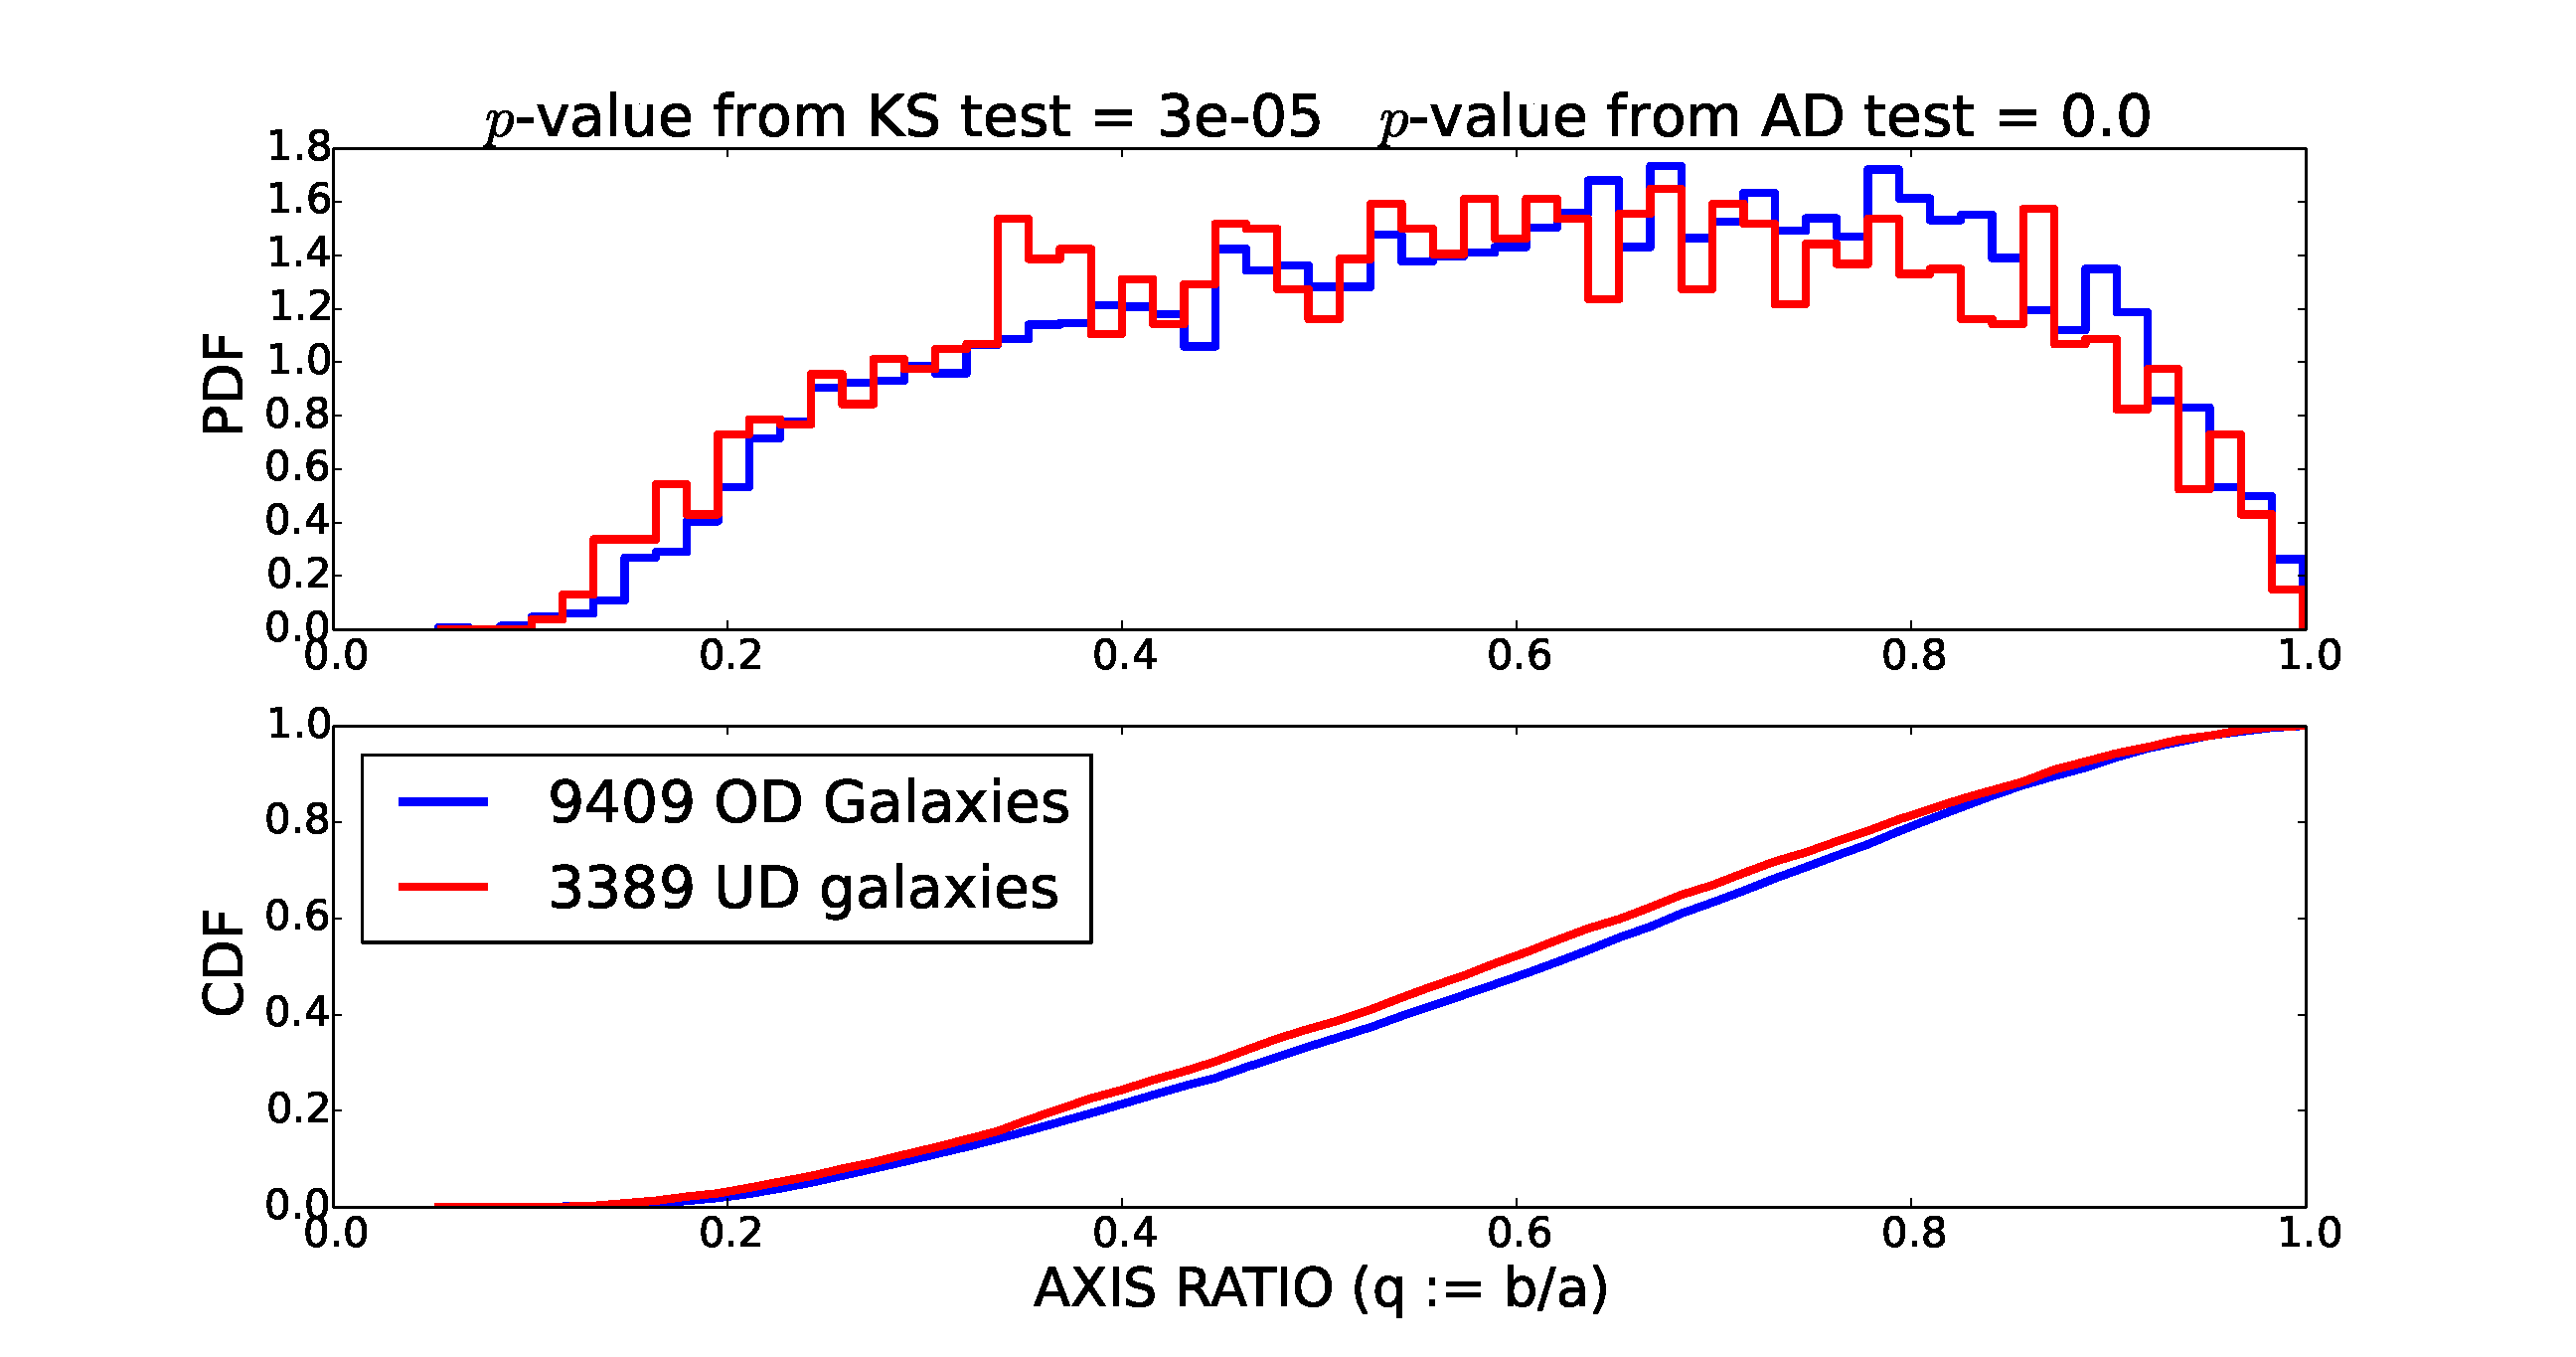
\includegraphics[width=0.66\columnwidth]{axis_ratio_all_Bbandevolution.eps}
 %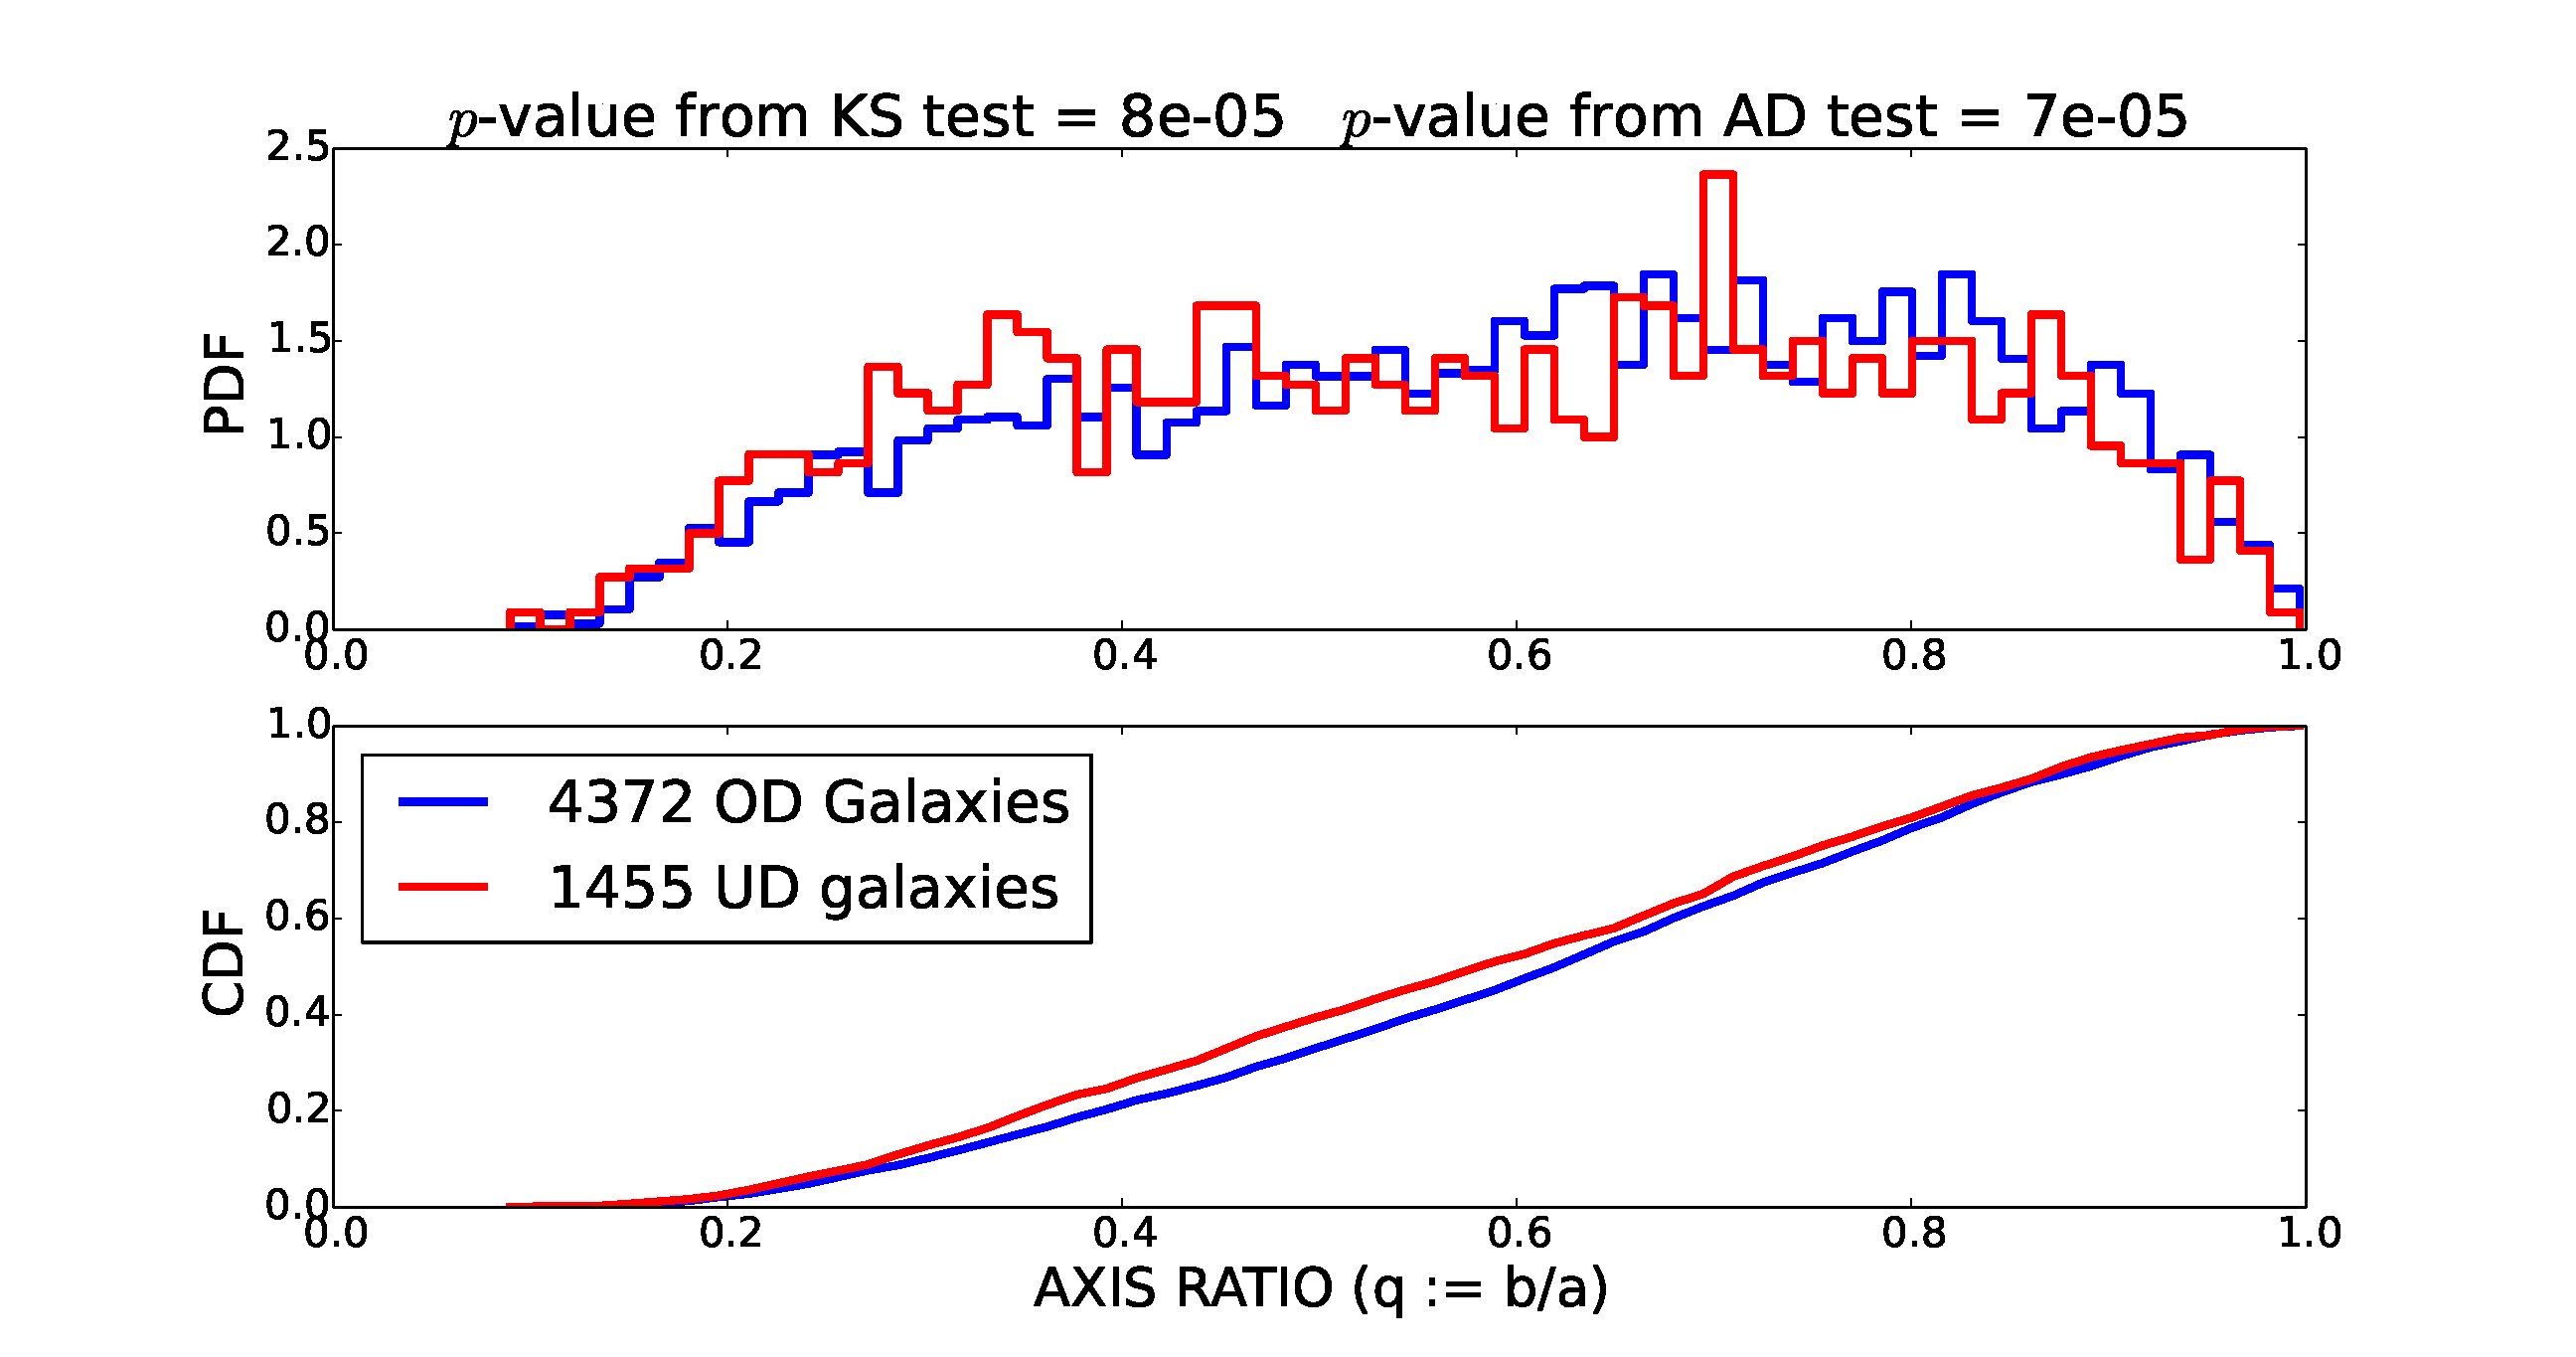
\includegraphics[width=0.66\columnwidth]{axis_ratio_all_masscut.eps}
 \caption{The distributions of axis ratios of galaxies in \emph{all} overdense (OD) and \emph{all} underdense (UD) regions in the case of luminosity-selected sample (left), luminosity-selected with B-band evolution taken into account (center) and stellar-mass-selected sample (right). The upper panels show the histogram
 and the botom panels show the empirical cumulative distribution function (ECDF). $p$-values are computed using these CDFs using the Kolmogorov-Smirnov and Anderson-Darling tests and are given in Table. \ref{table:pvalues_all}. The difference between the CDFs turn out to be statistically significant. \rachel{This figure and the ones below appear to be right-justified (pushed up against the right margin) instead of centered.  Can you look into fixing that?  Also, the $:=$ is not very standard notation, I recommend just $=$.  Finally, the spacing in the legends is funny; I would prefer to see things like ``8213 (OD)'' rather than the current ``8213( OD )''.  The former is also consistent with the next figure.}}
 \label{fig:axisratio_all}
\end{figure*}

\begin{figure*}
 \centering
 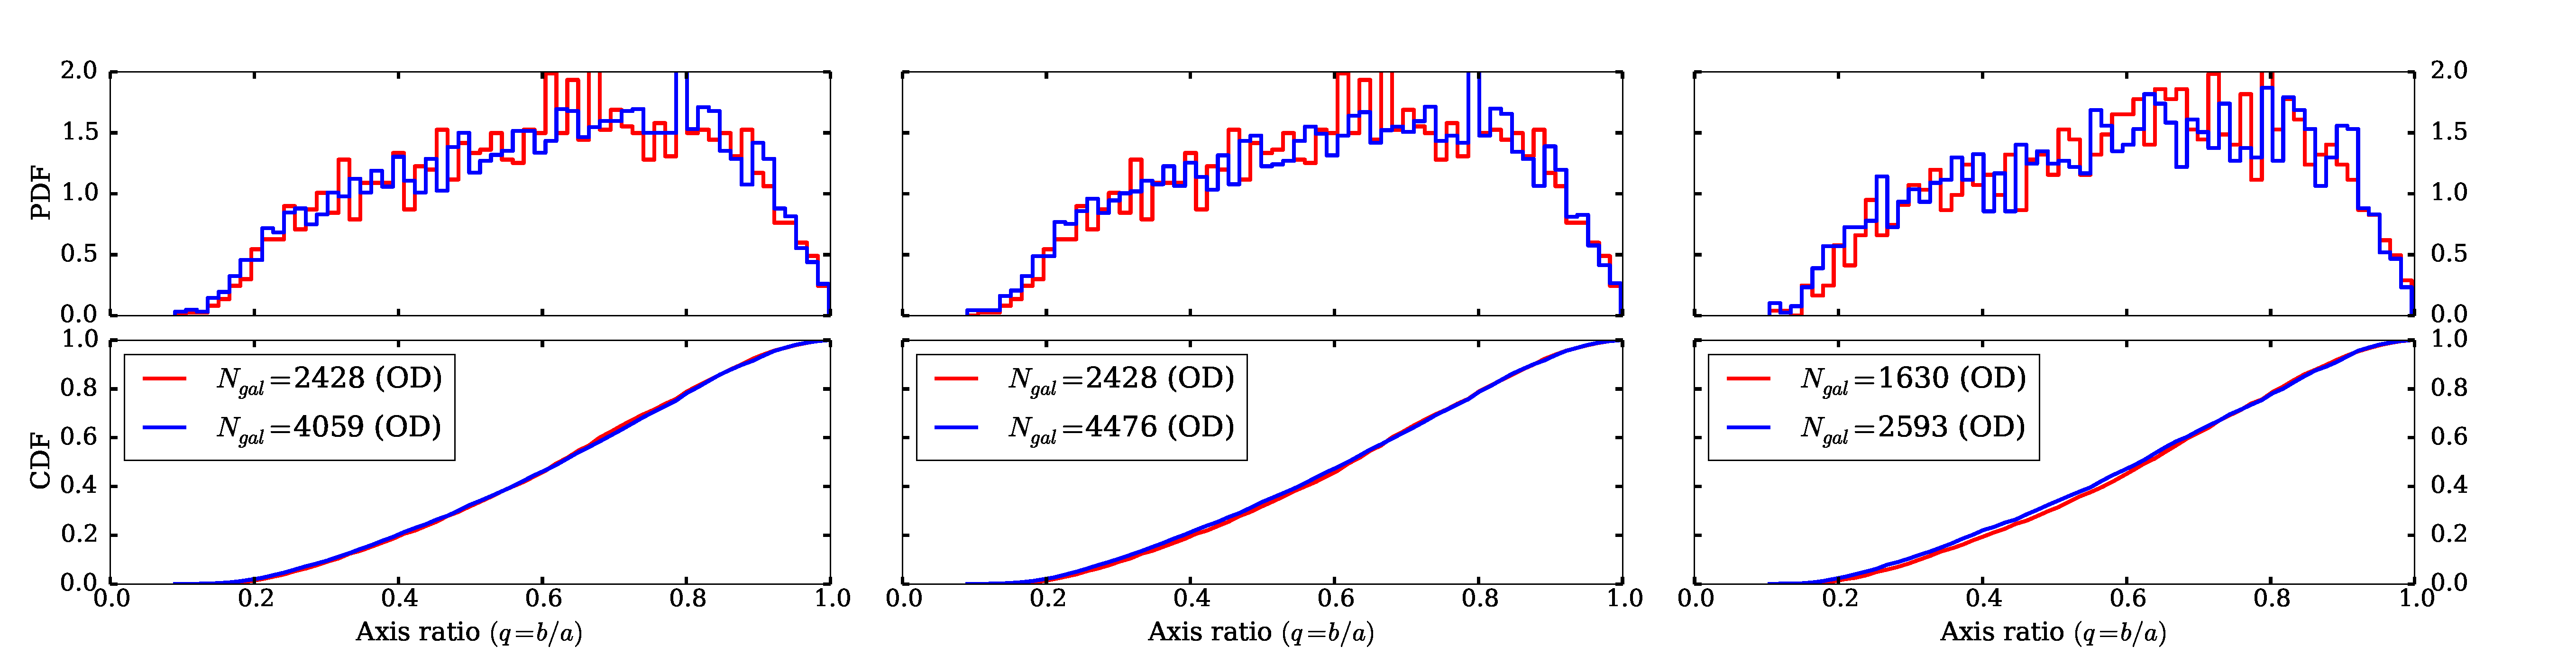
\includegraphics[width=2.3\columnwidth]{axis_ratio_odod}
 %a) 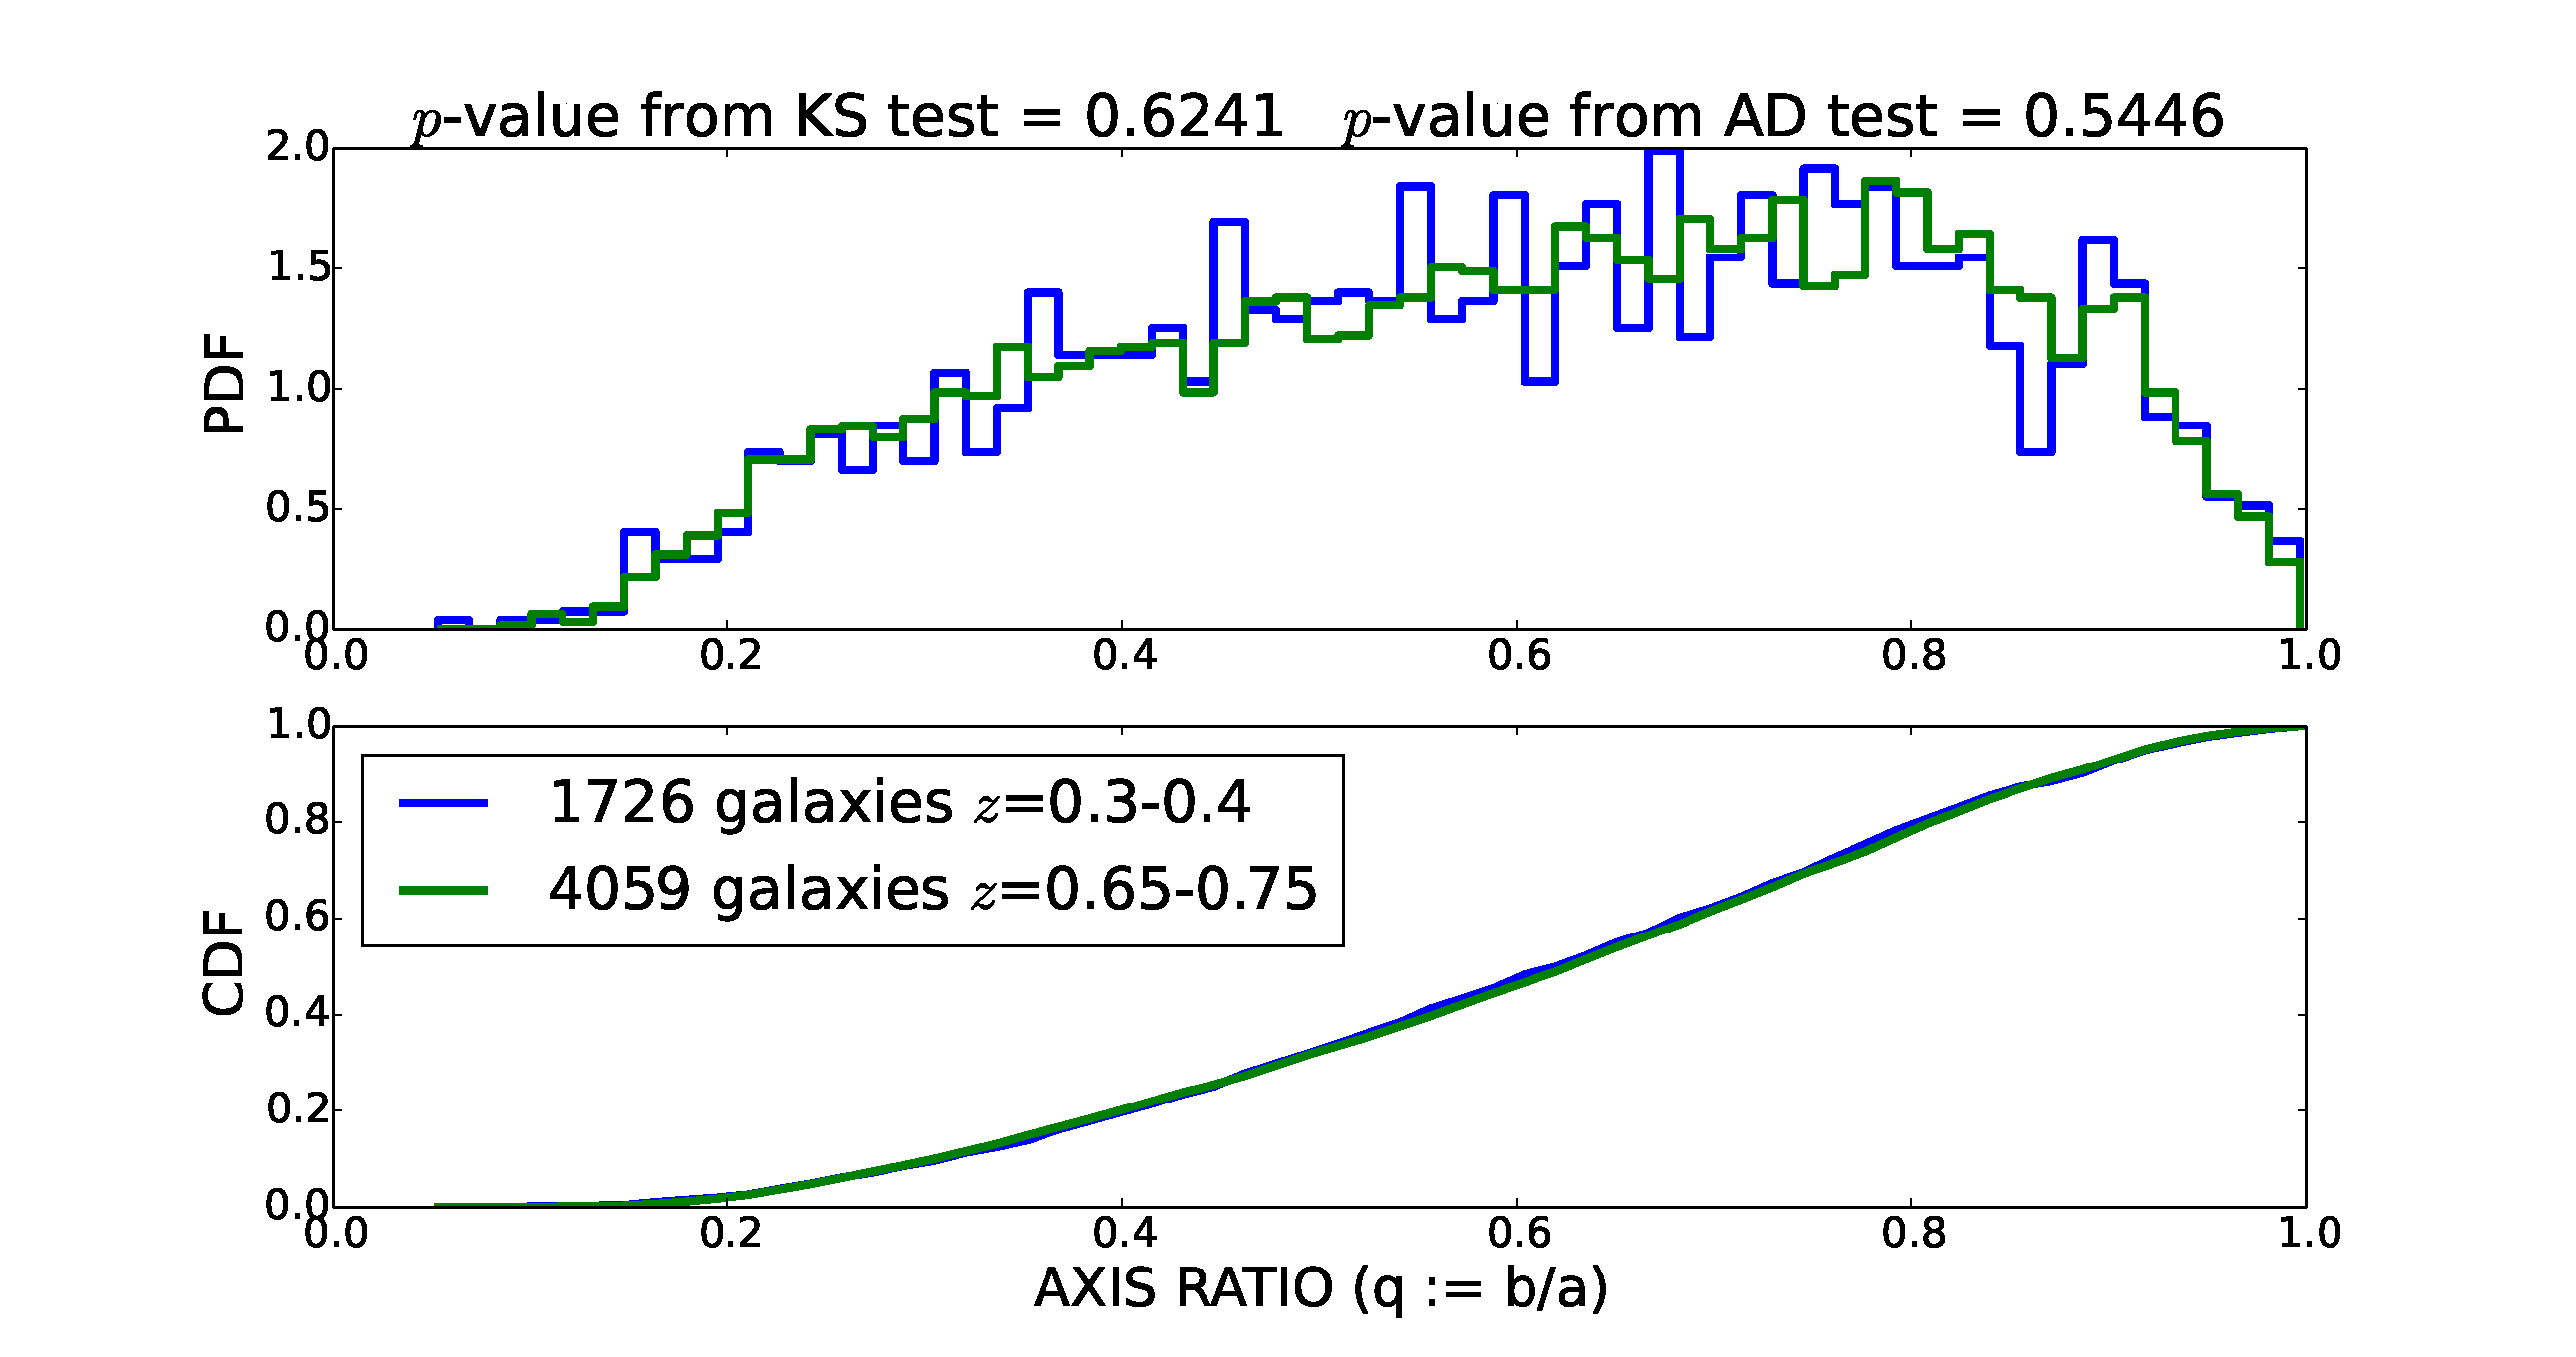
\includegraphics[width=0.9\columnwidth]{axisratio(0)_0dot3-0dot4_0dot65-0dot75.eps} \
 %b) 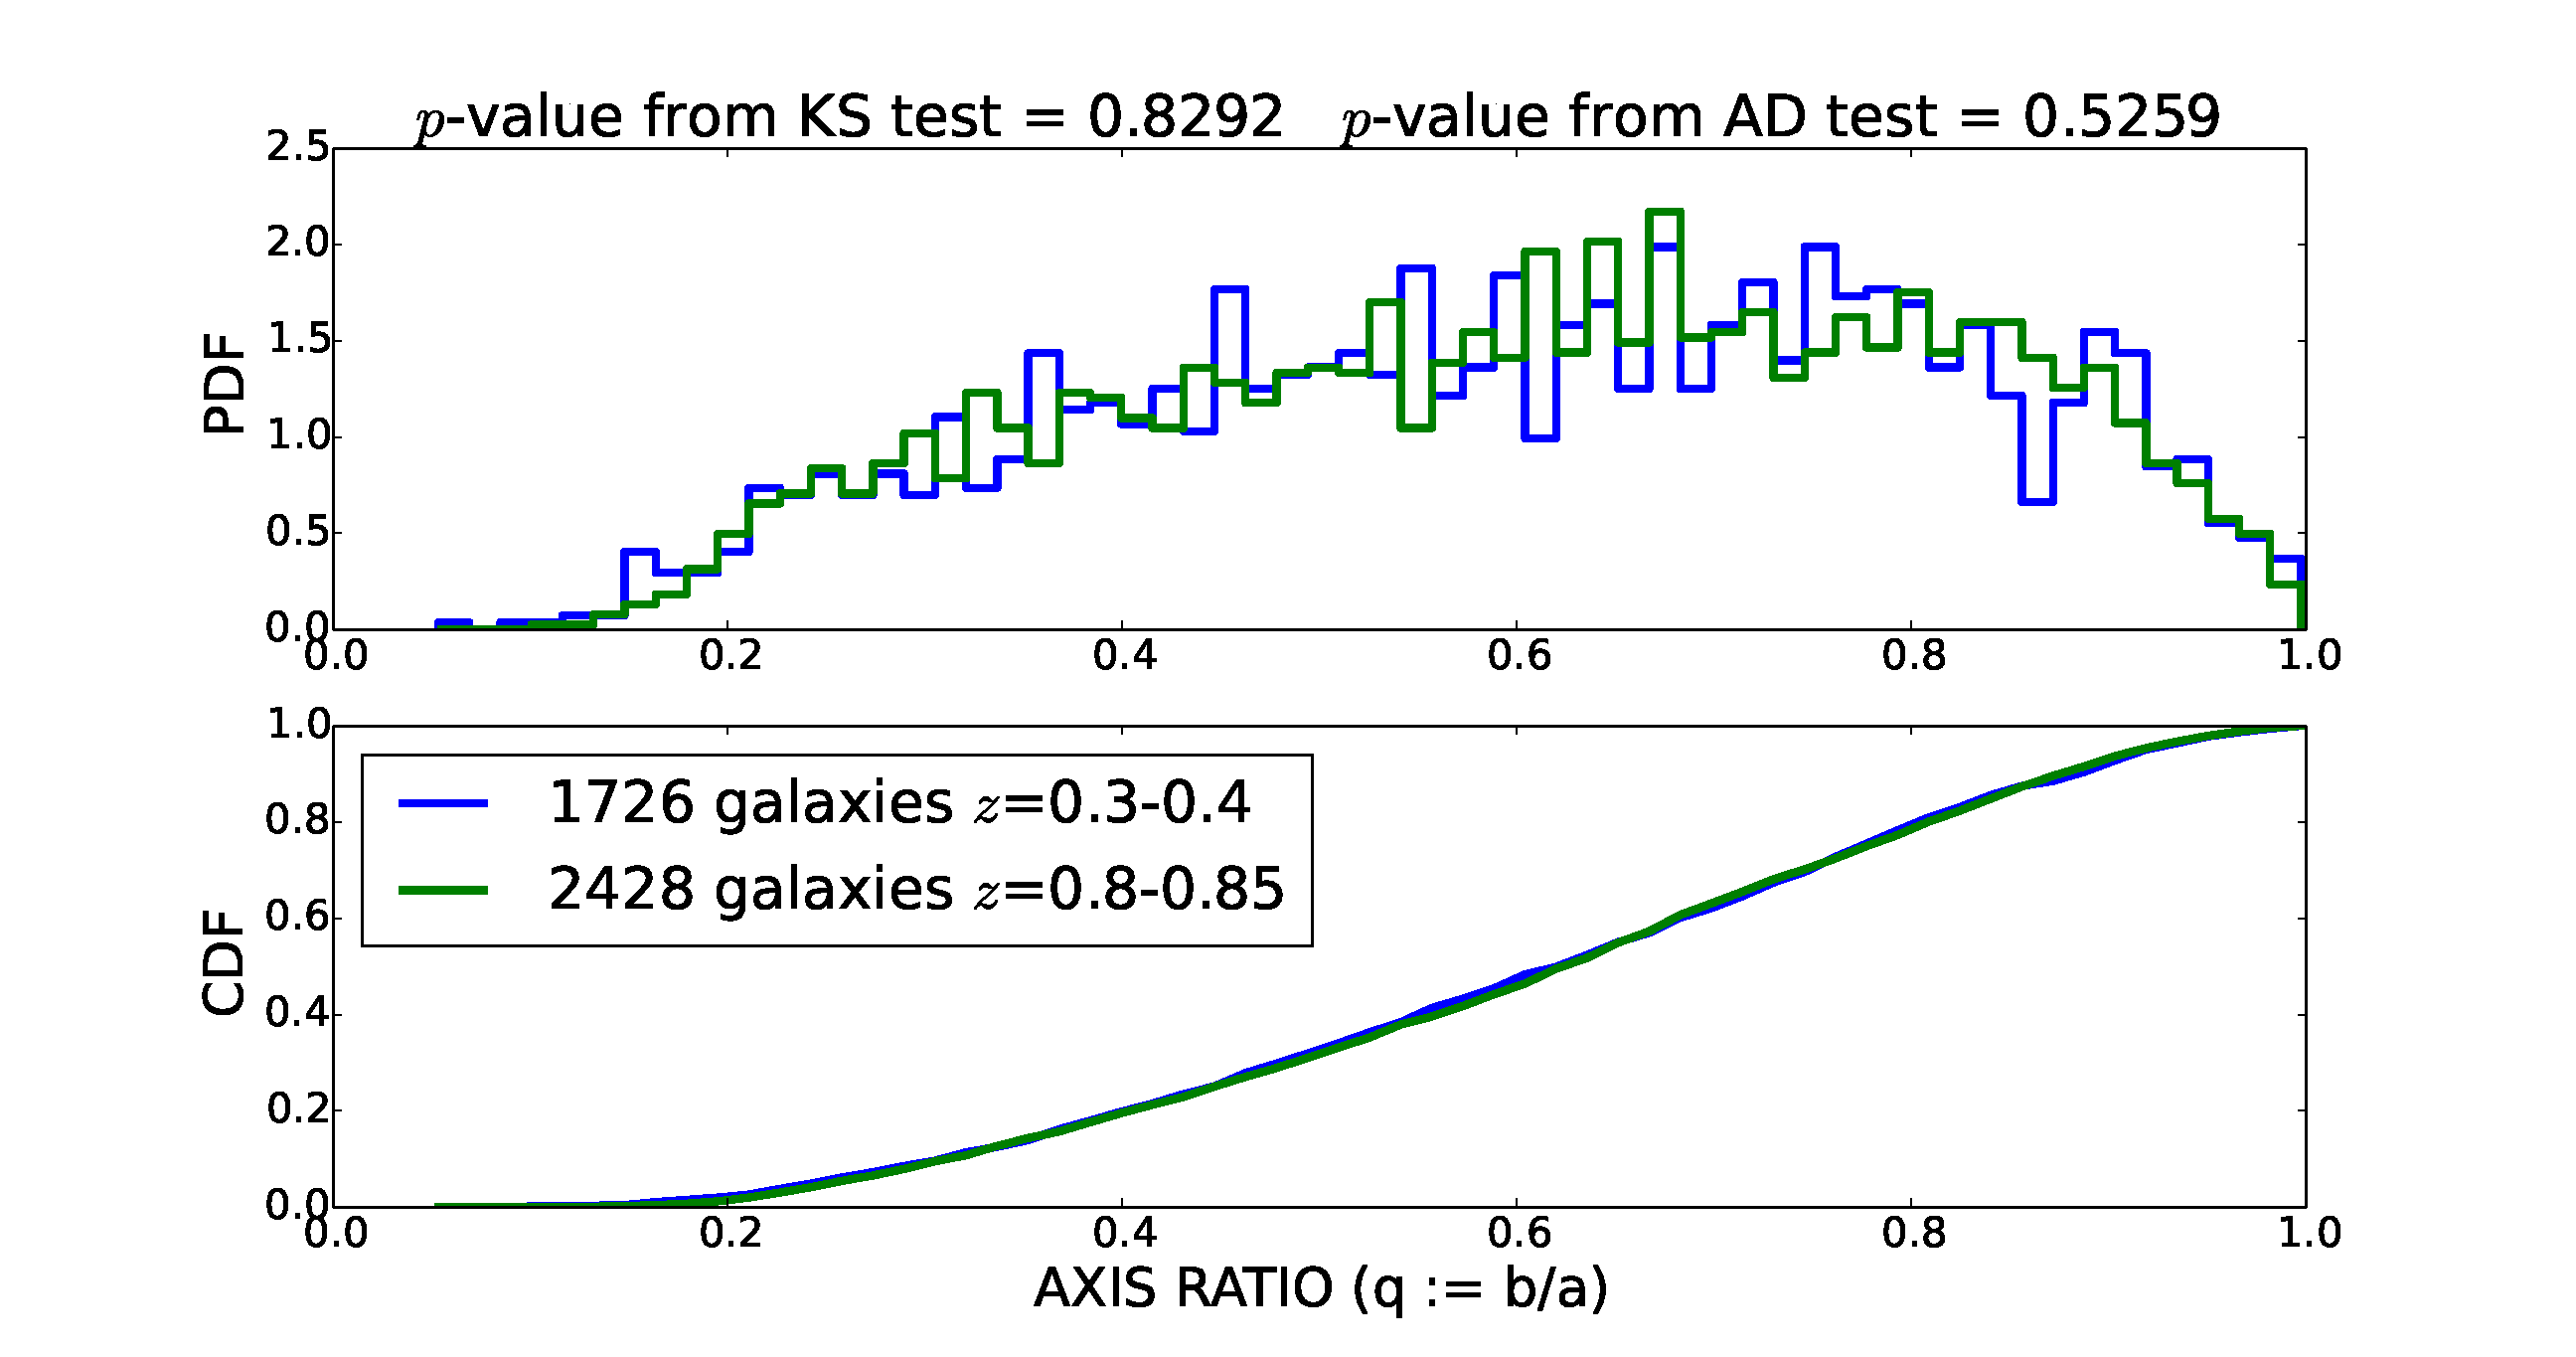
\includegraphics[width=0.9\columnwidth]{axisratio(0)_0dot3-0dot4_0dot80-0dot85.eps} \\
 %c) 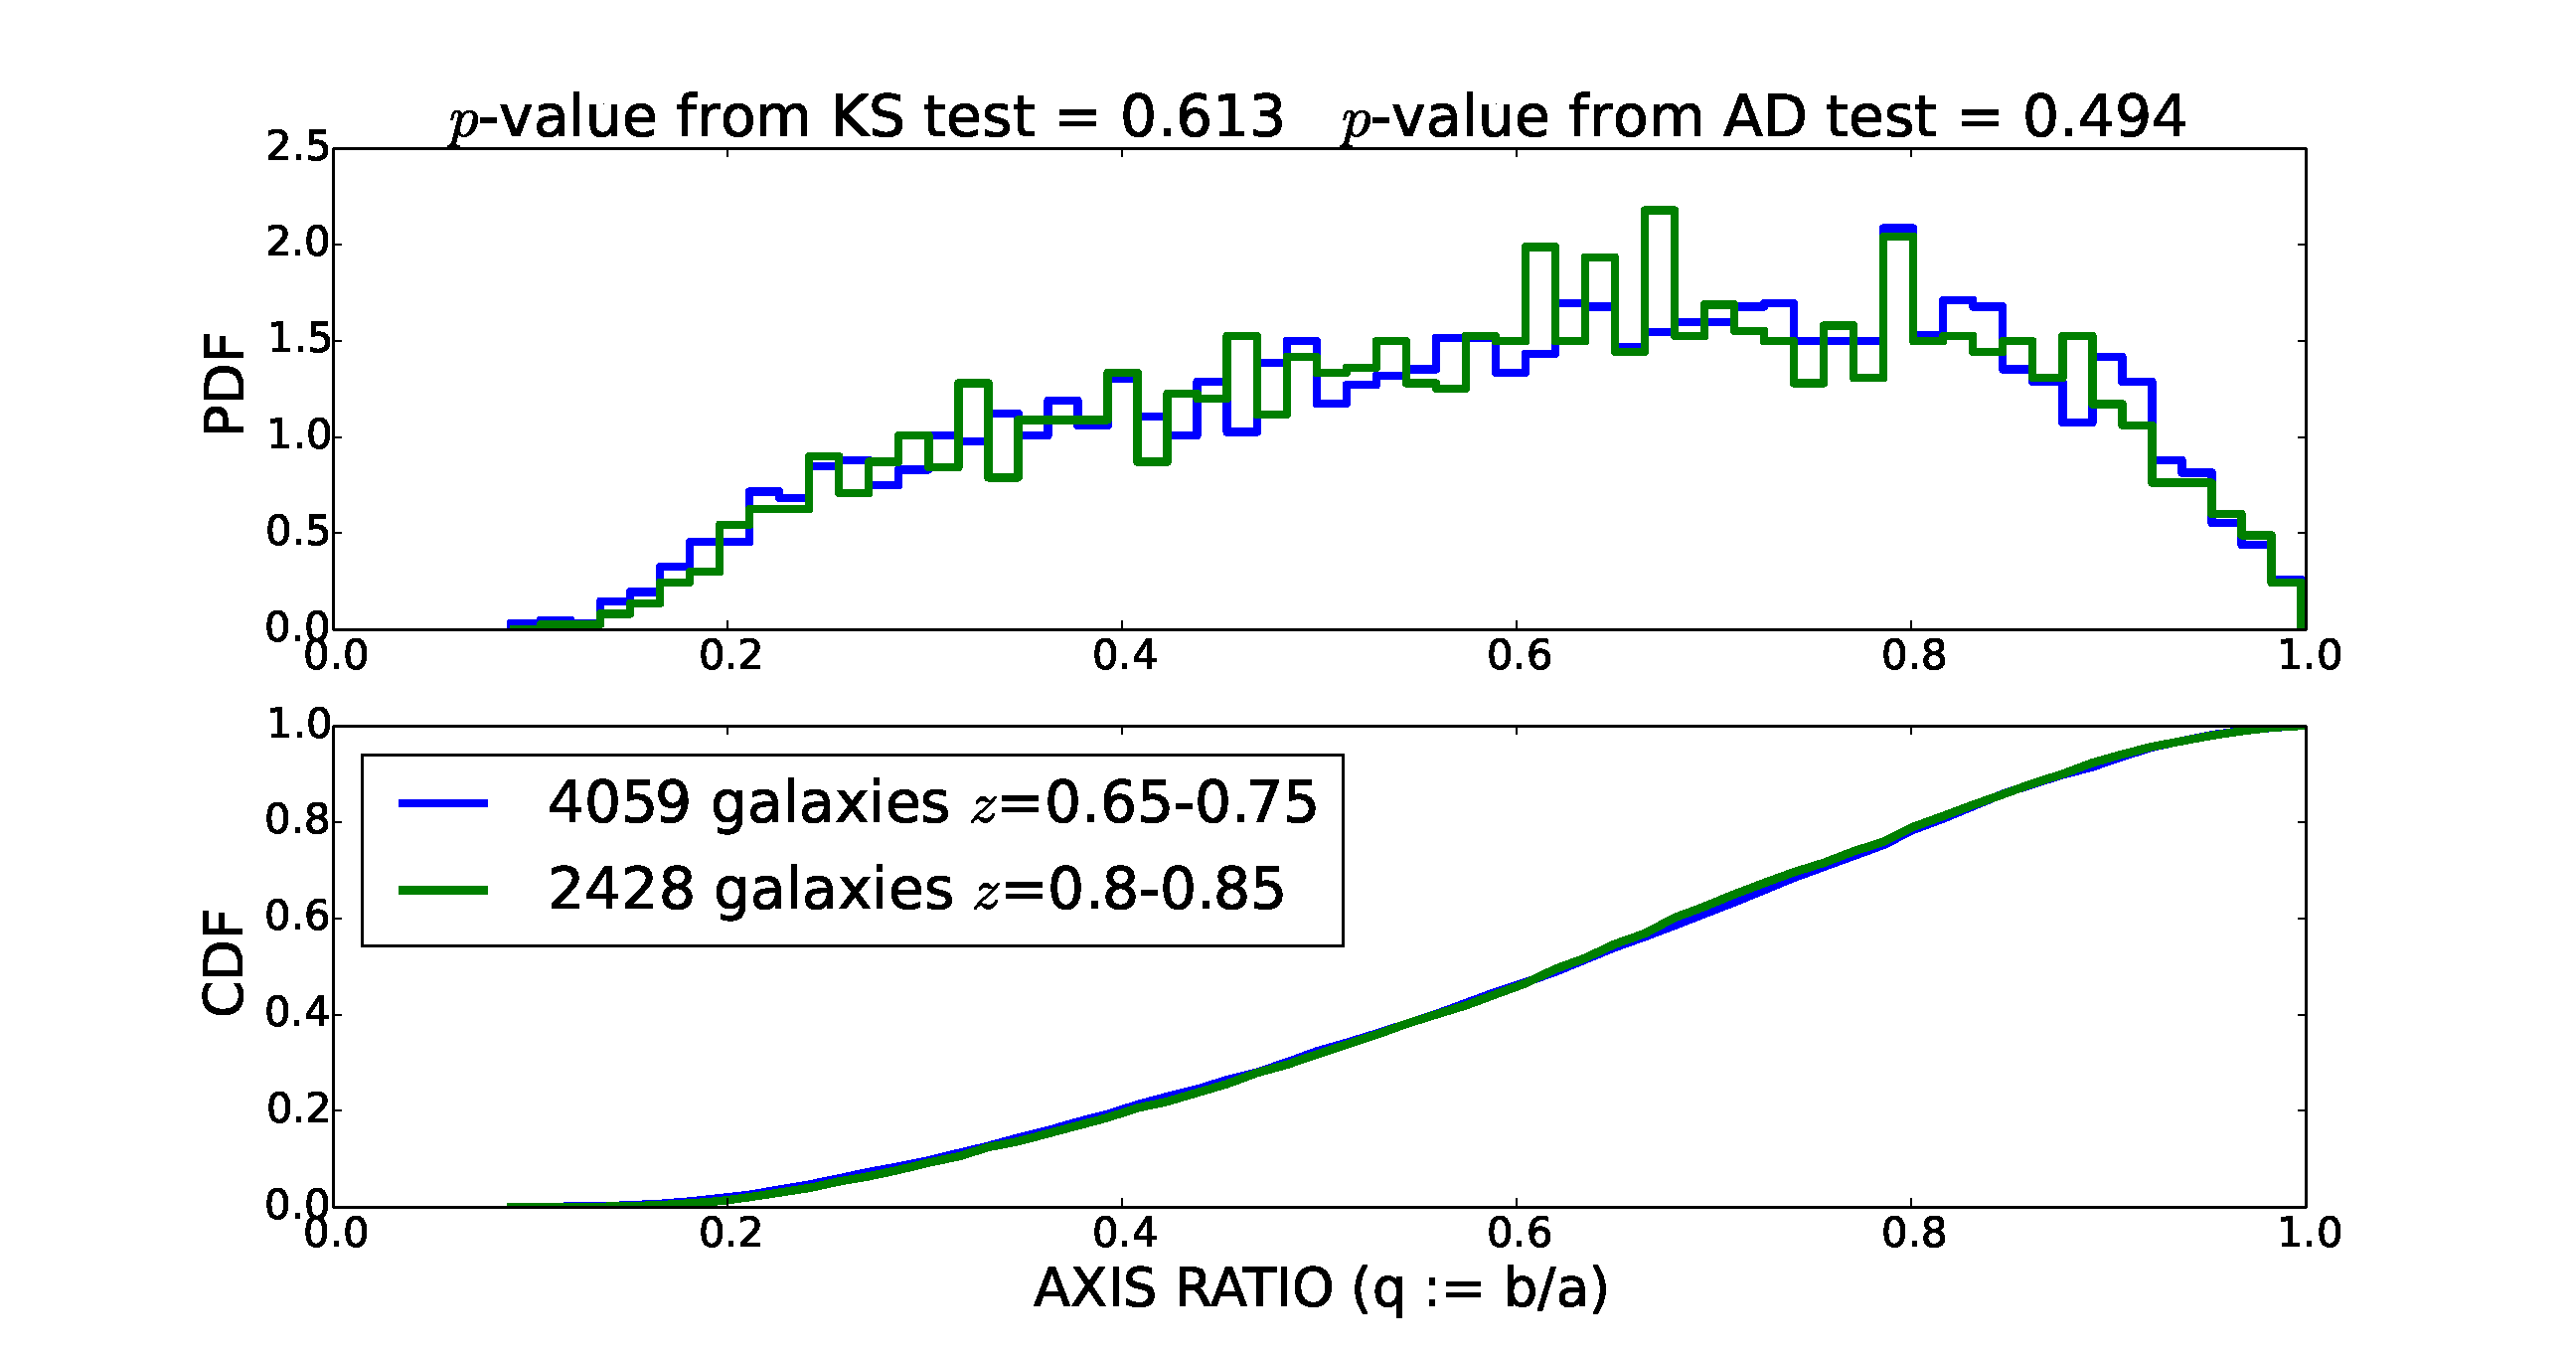
\includegraphics[width=0.9\columnwidth]{axisratio(0)_0dot65-0dot75_0dot80-0dot85.eps} \
 %d) 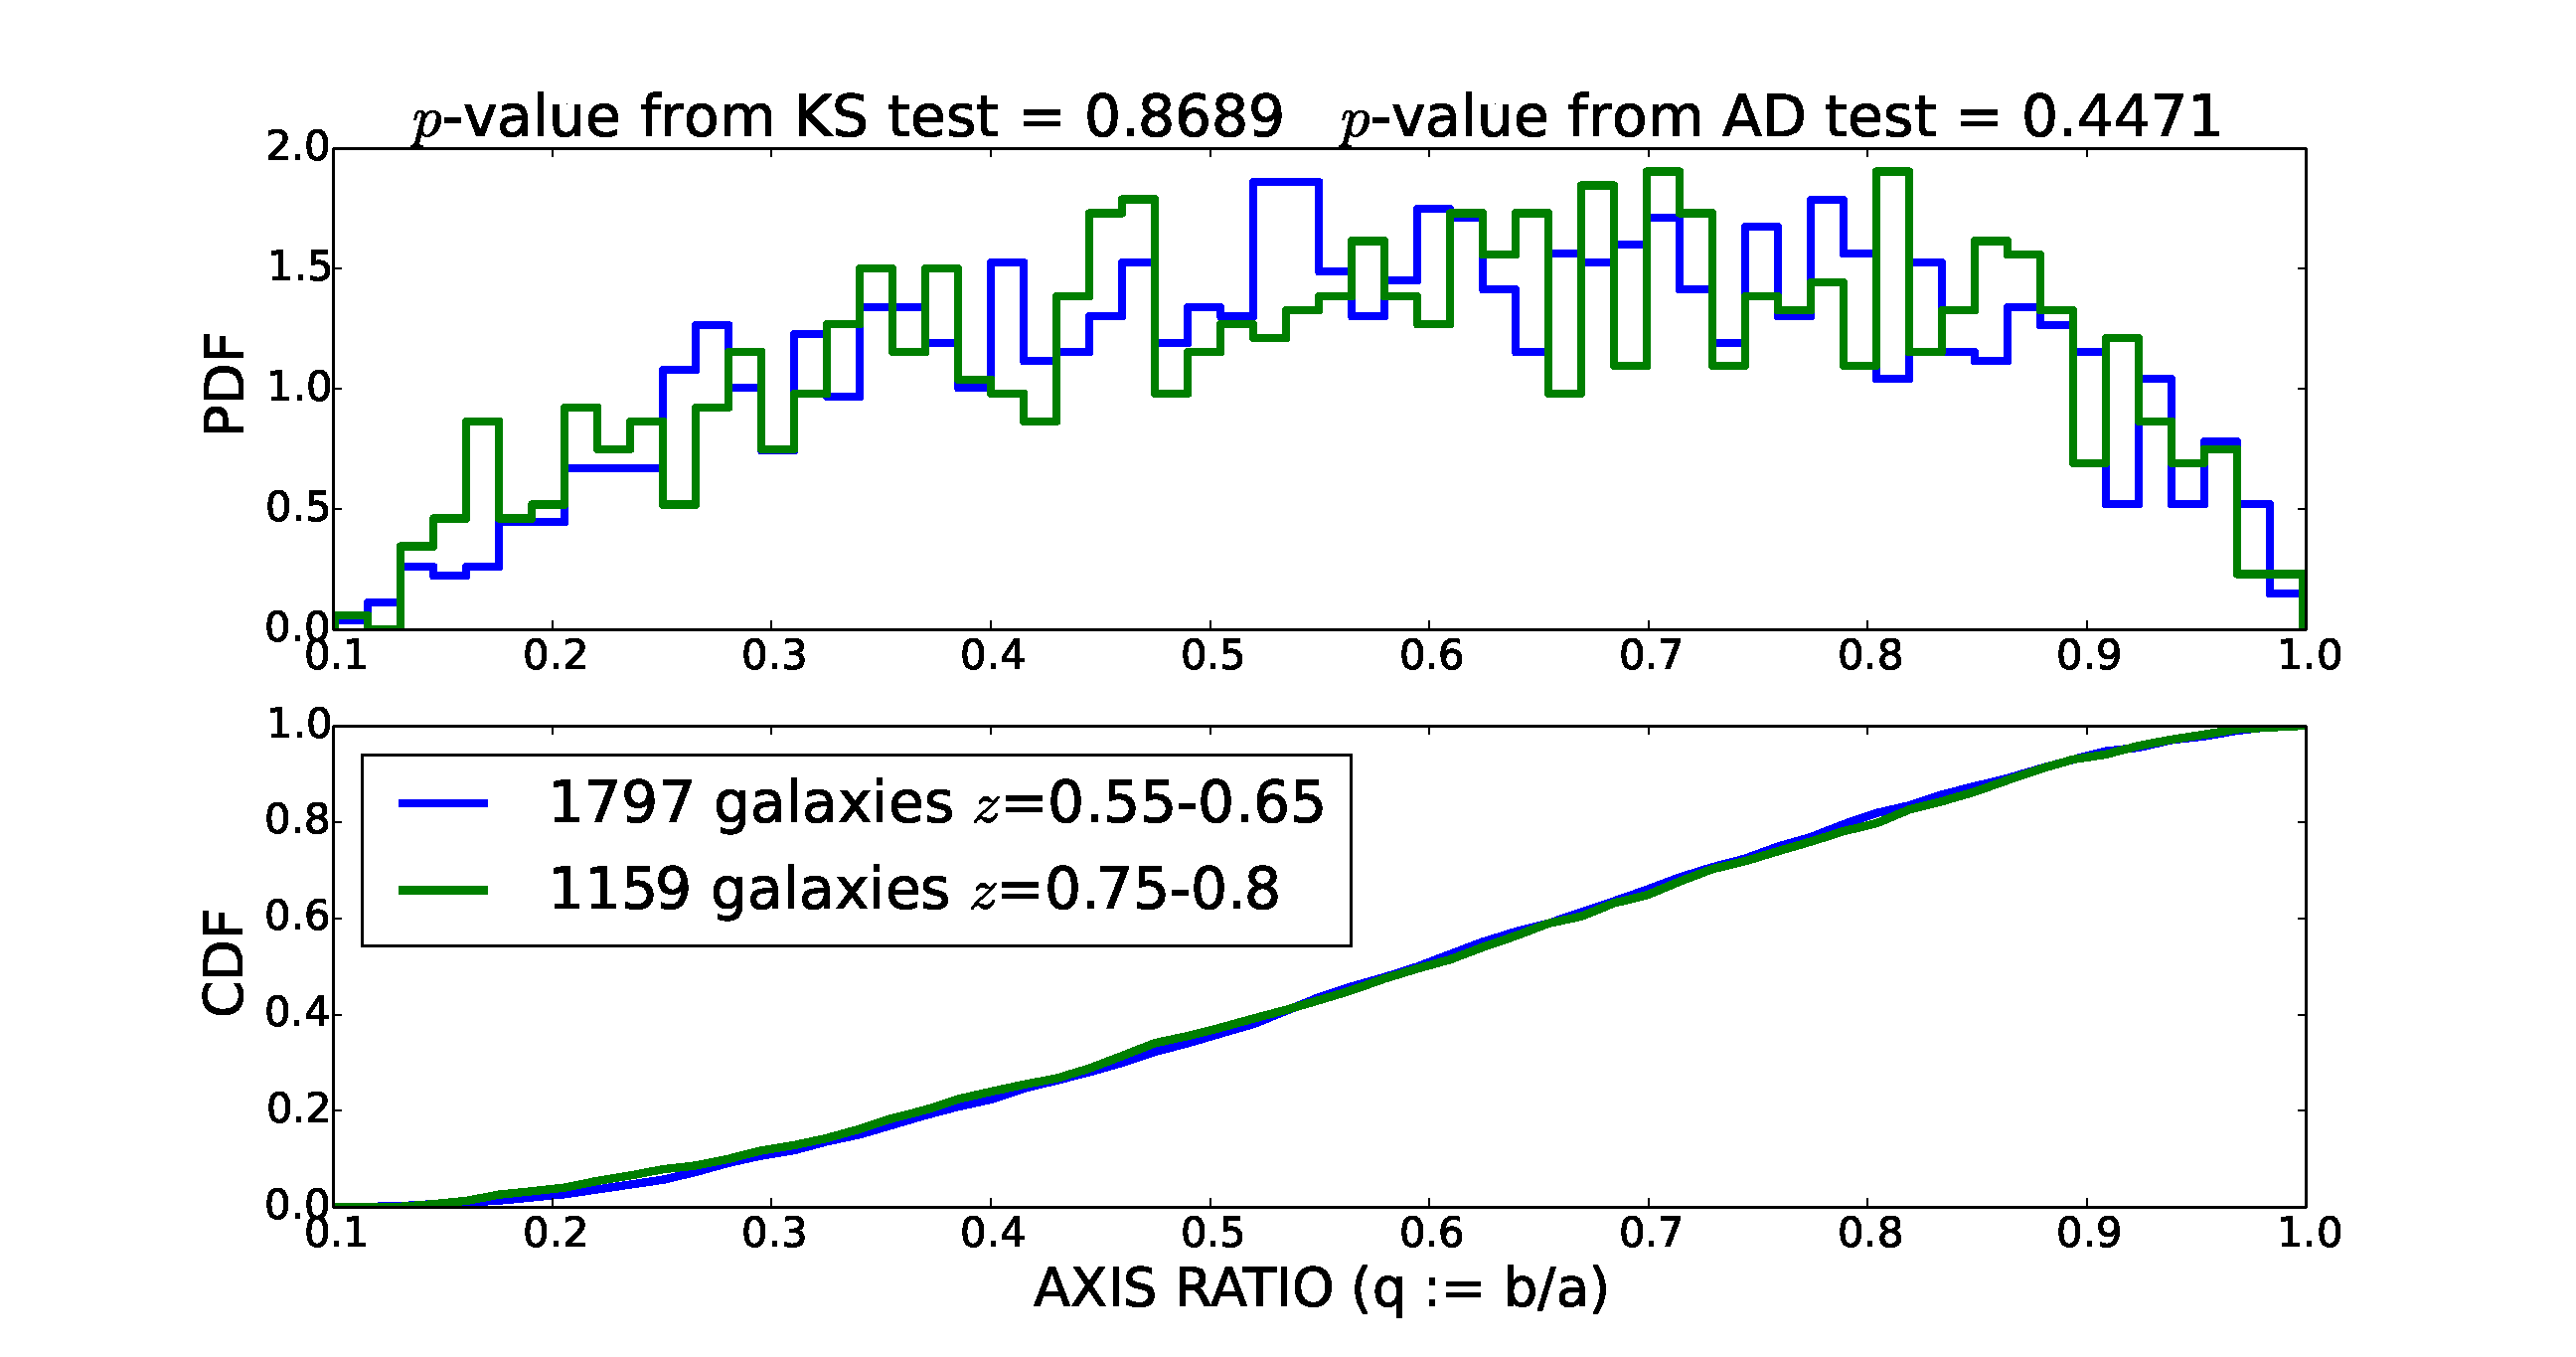
\includegraphics[width=0.9\columnwidth]{axisratio(0)_0dot55-0dot65_0dot75-0dot8.eps} \
 \caption{Comparison in similar environments: Axis ratios of galaxies in two overdense redshift bins, $z=0.65-0.75$ and $z=0.80-0.85$ are compared. $p$-values from the KS and AD test are given in Table.~\ref{table:pvalues_all}}
 \label{fig:axisratio_similar}
\end{figure*}

\begin{figure*}
 \centering
 \includegraphics[width=2.3\columnwidth]{axis_ratio_odud}
 %a) 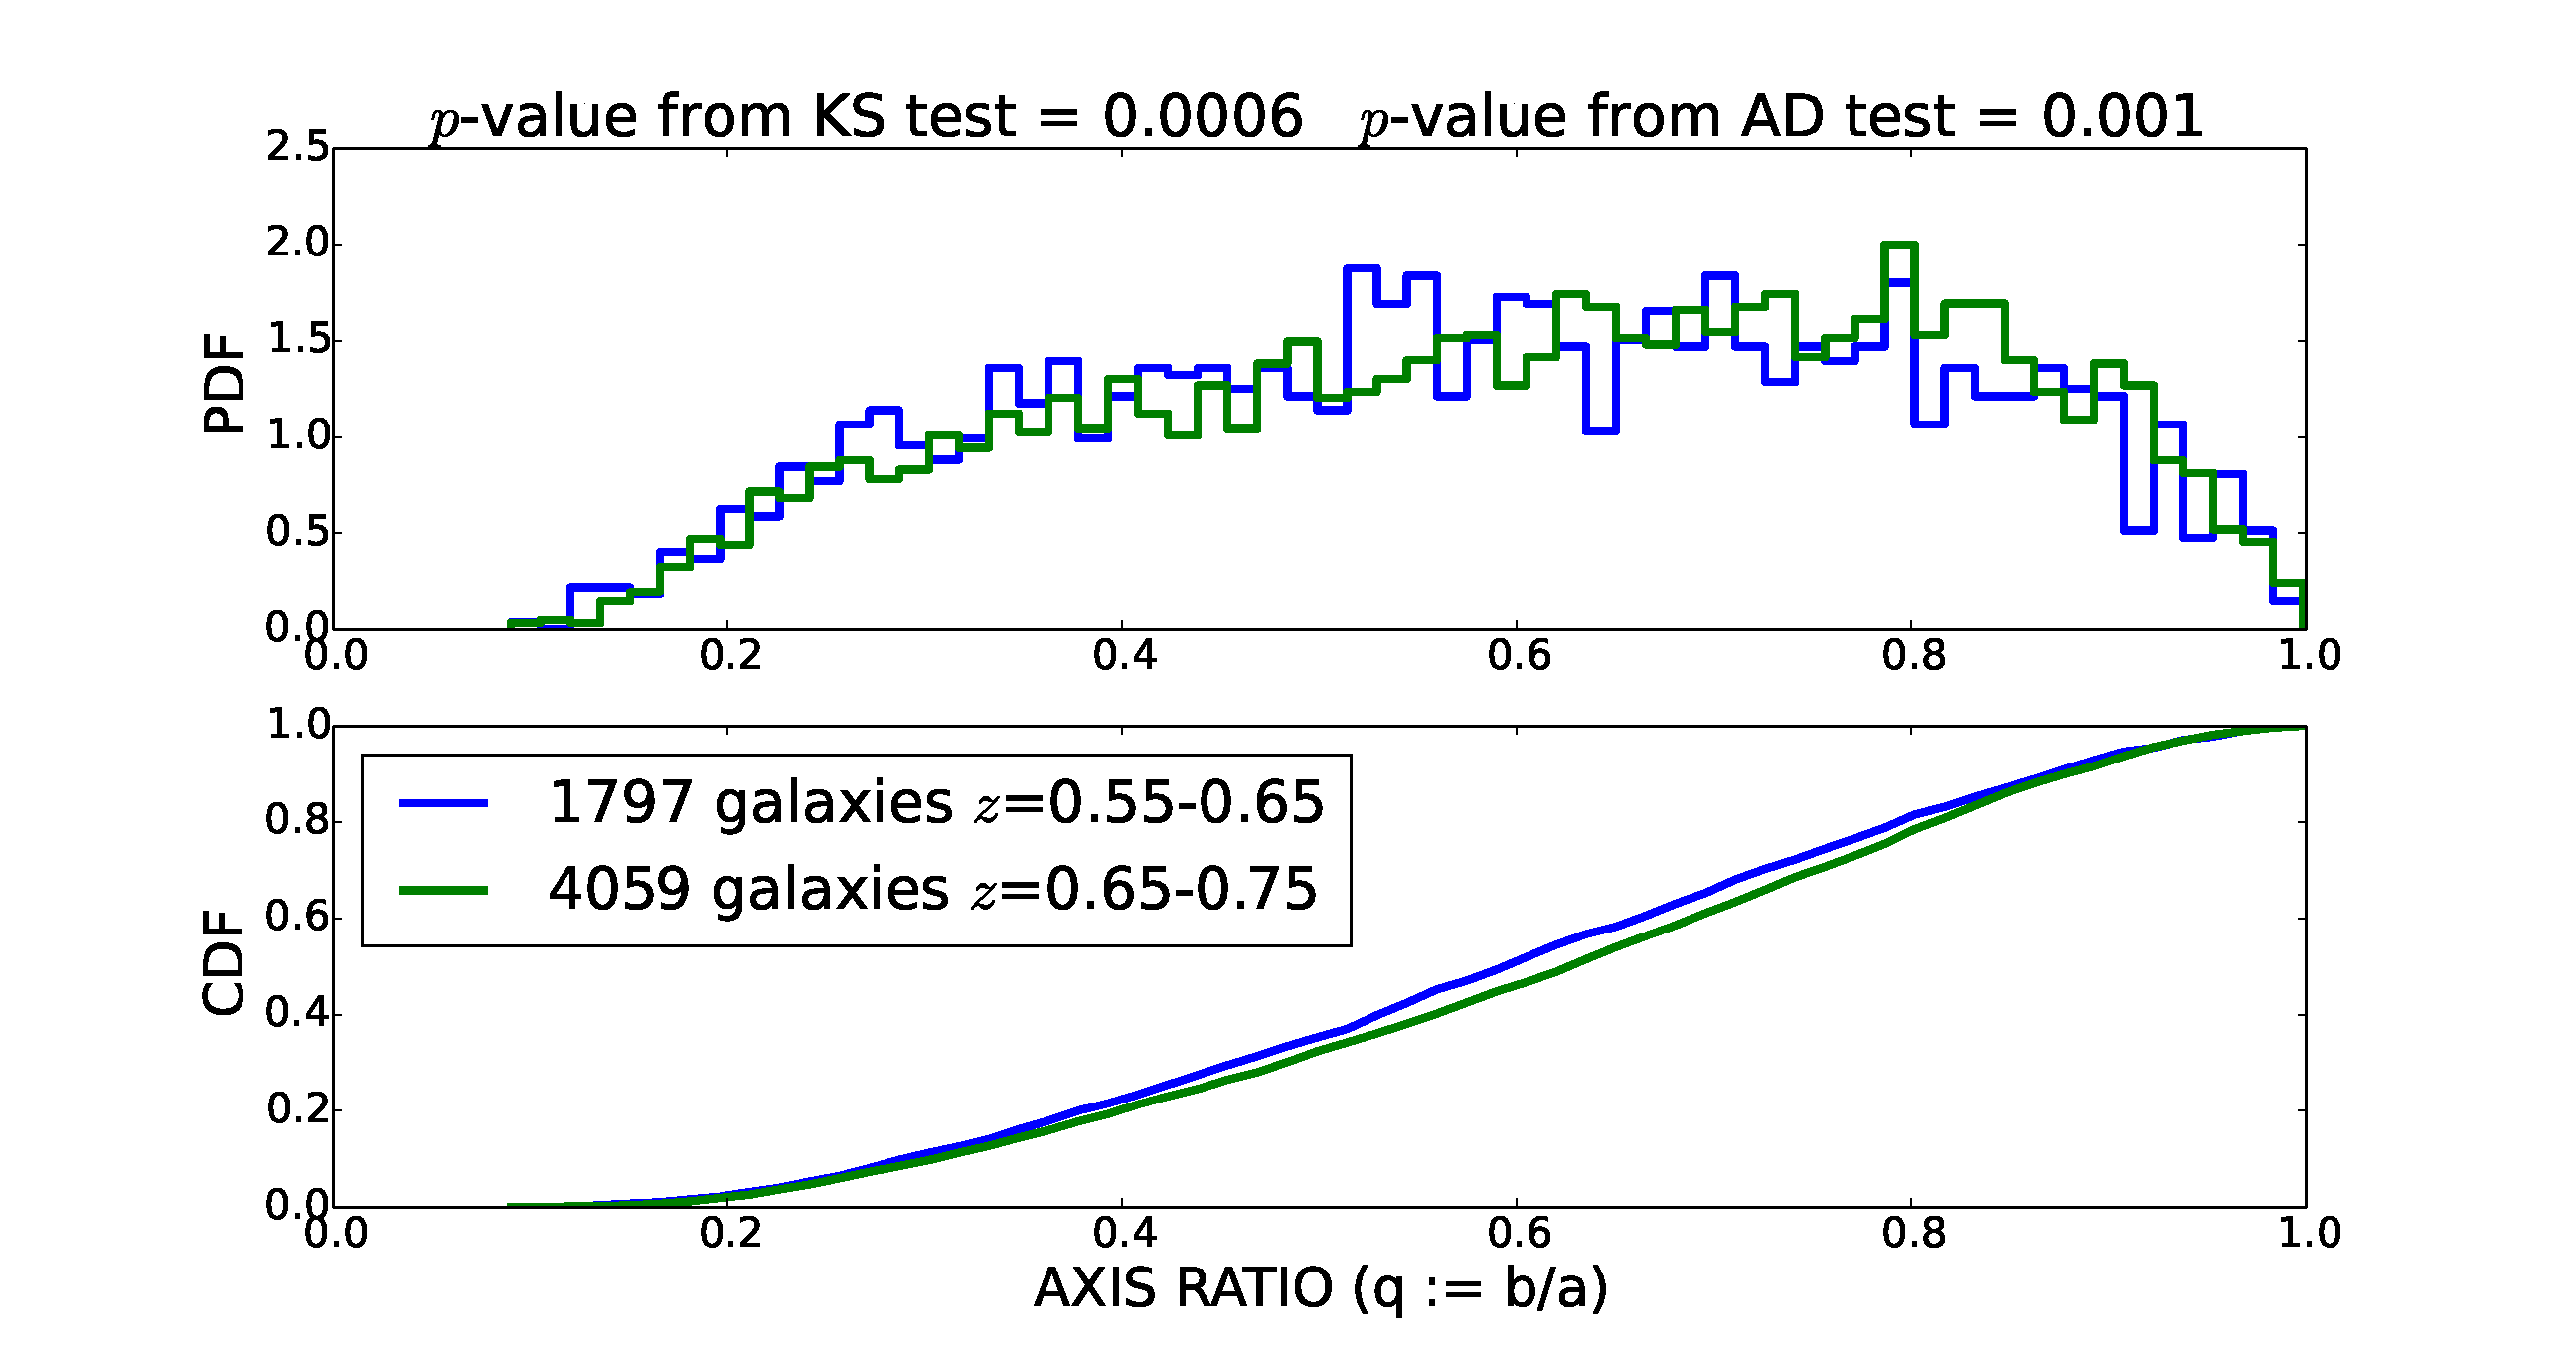
\includegraphics[width=0.9\columnwidth]{axisratio(0)_0dot55-0dot65_0dot65-0dot75.eps} \
 %#b) 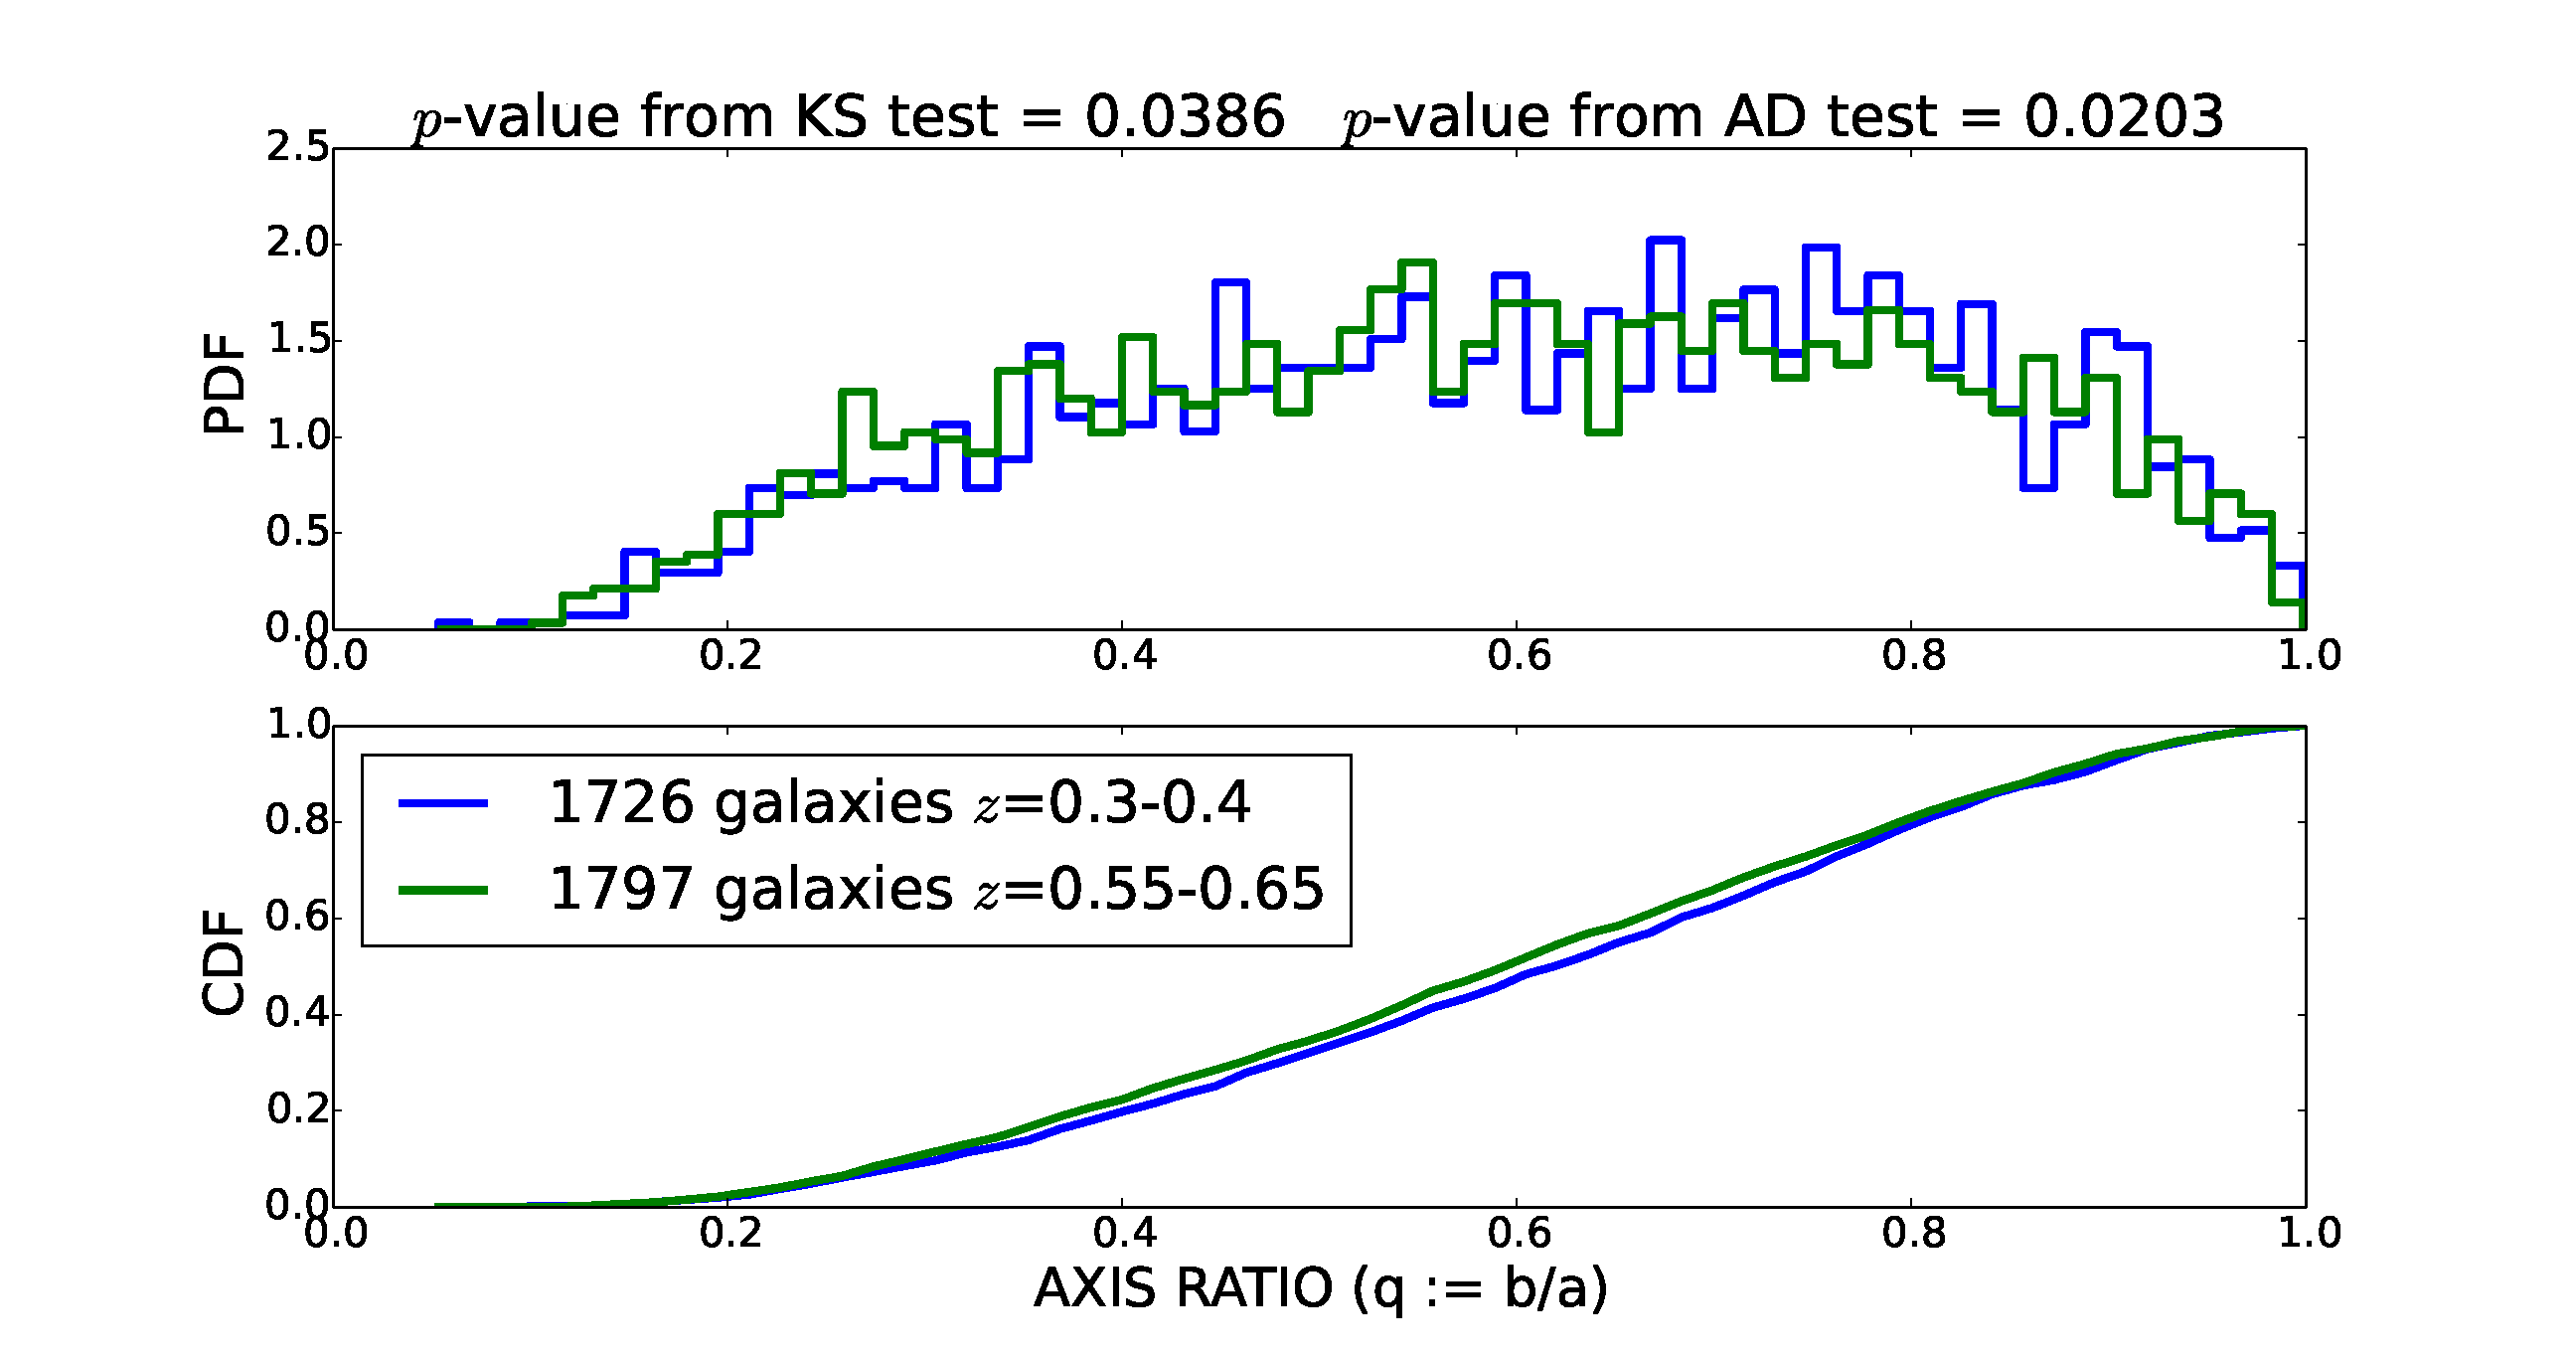
\includegraphics[width=0.9\columnwidth]{axisratio(0)_0dot3-0dot4_0dot55-0dot65.eps} \\
 %c) 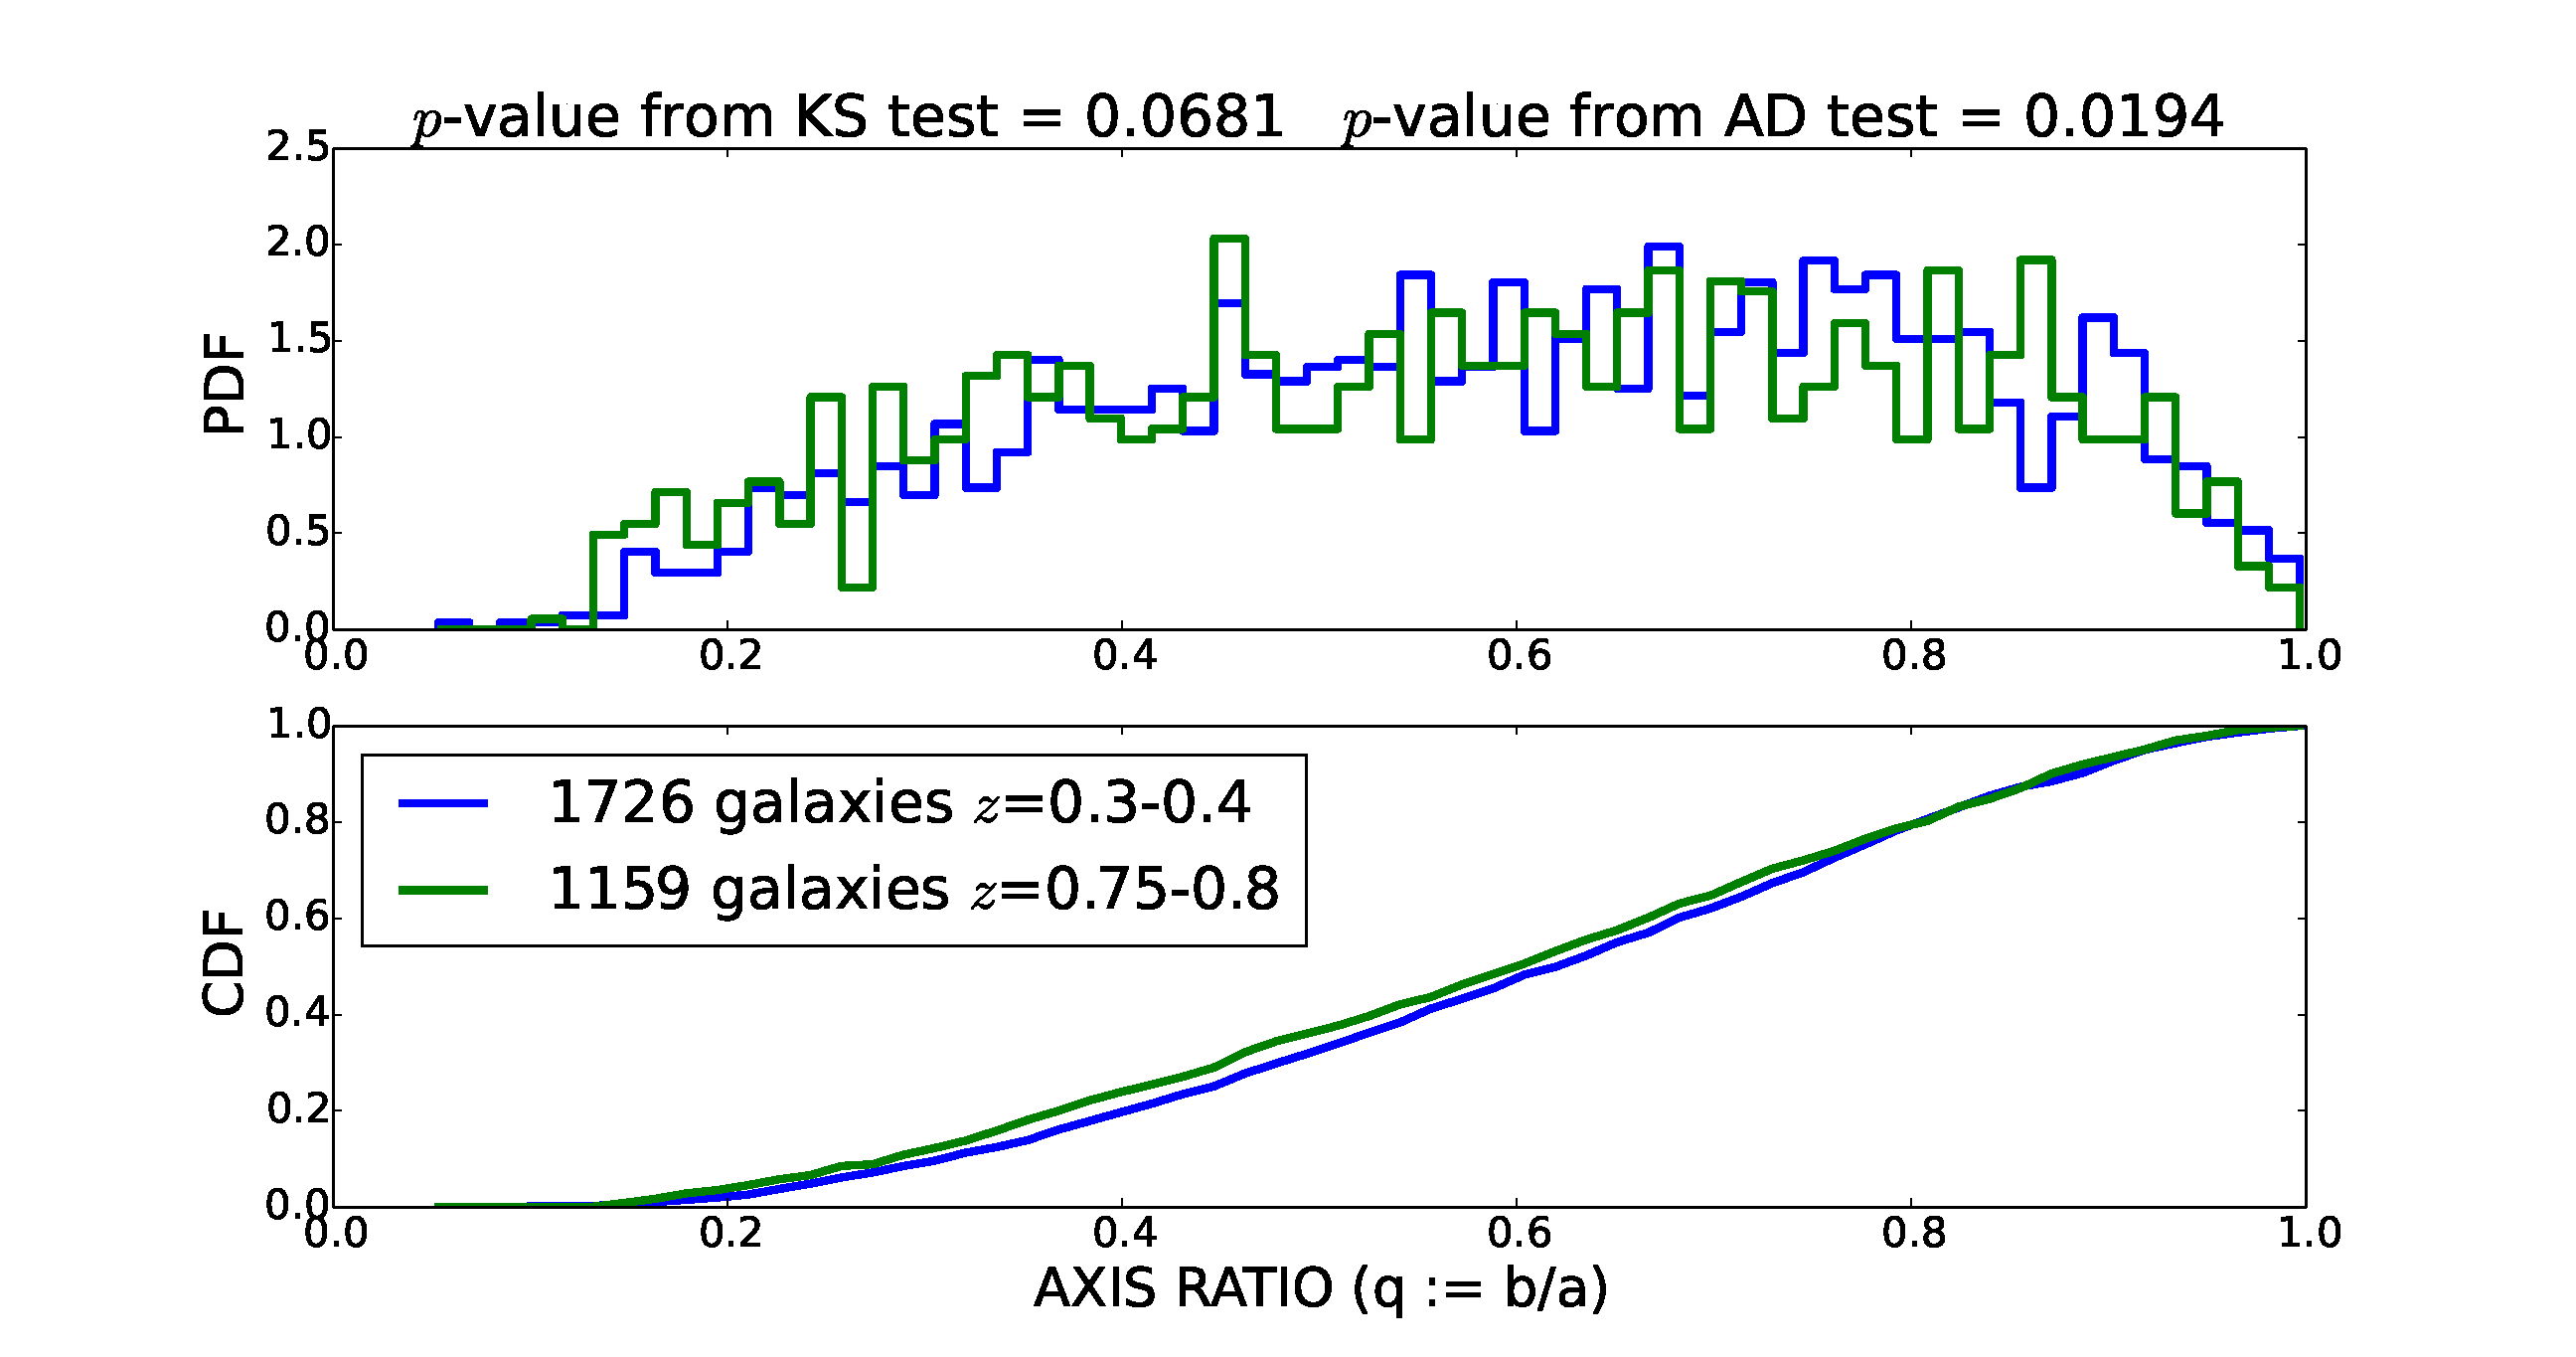
\includegraphics[width=0.9\columnwidth]{axisratio(0)_0dot3-0dot4_0dot75-0dot8.eps} \
 %d) 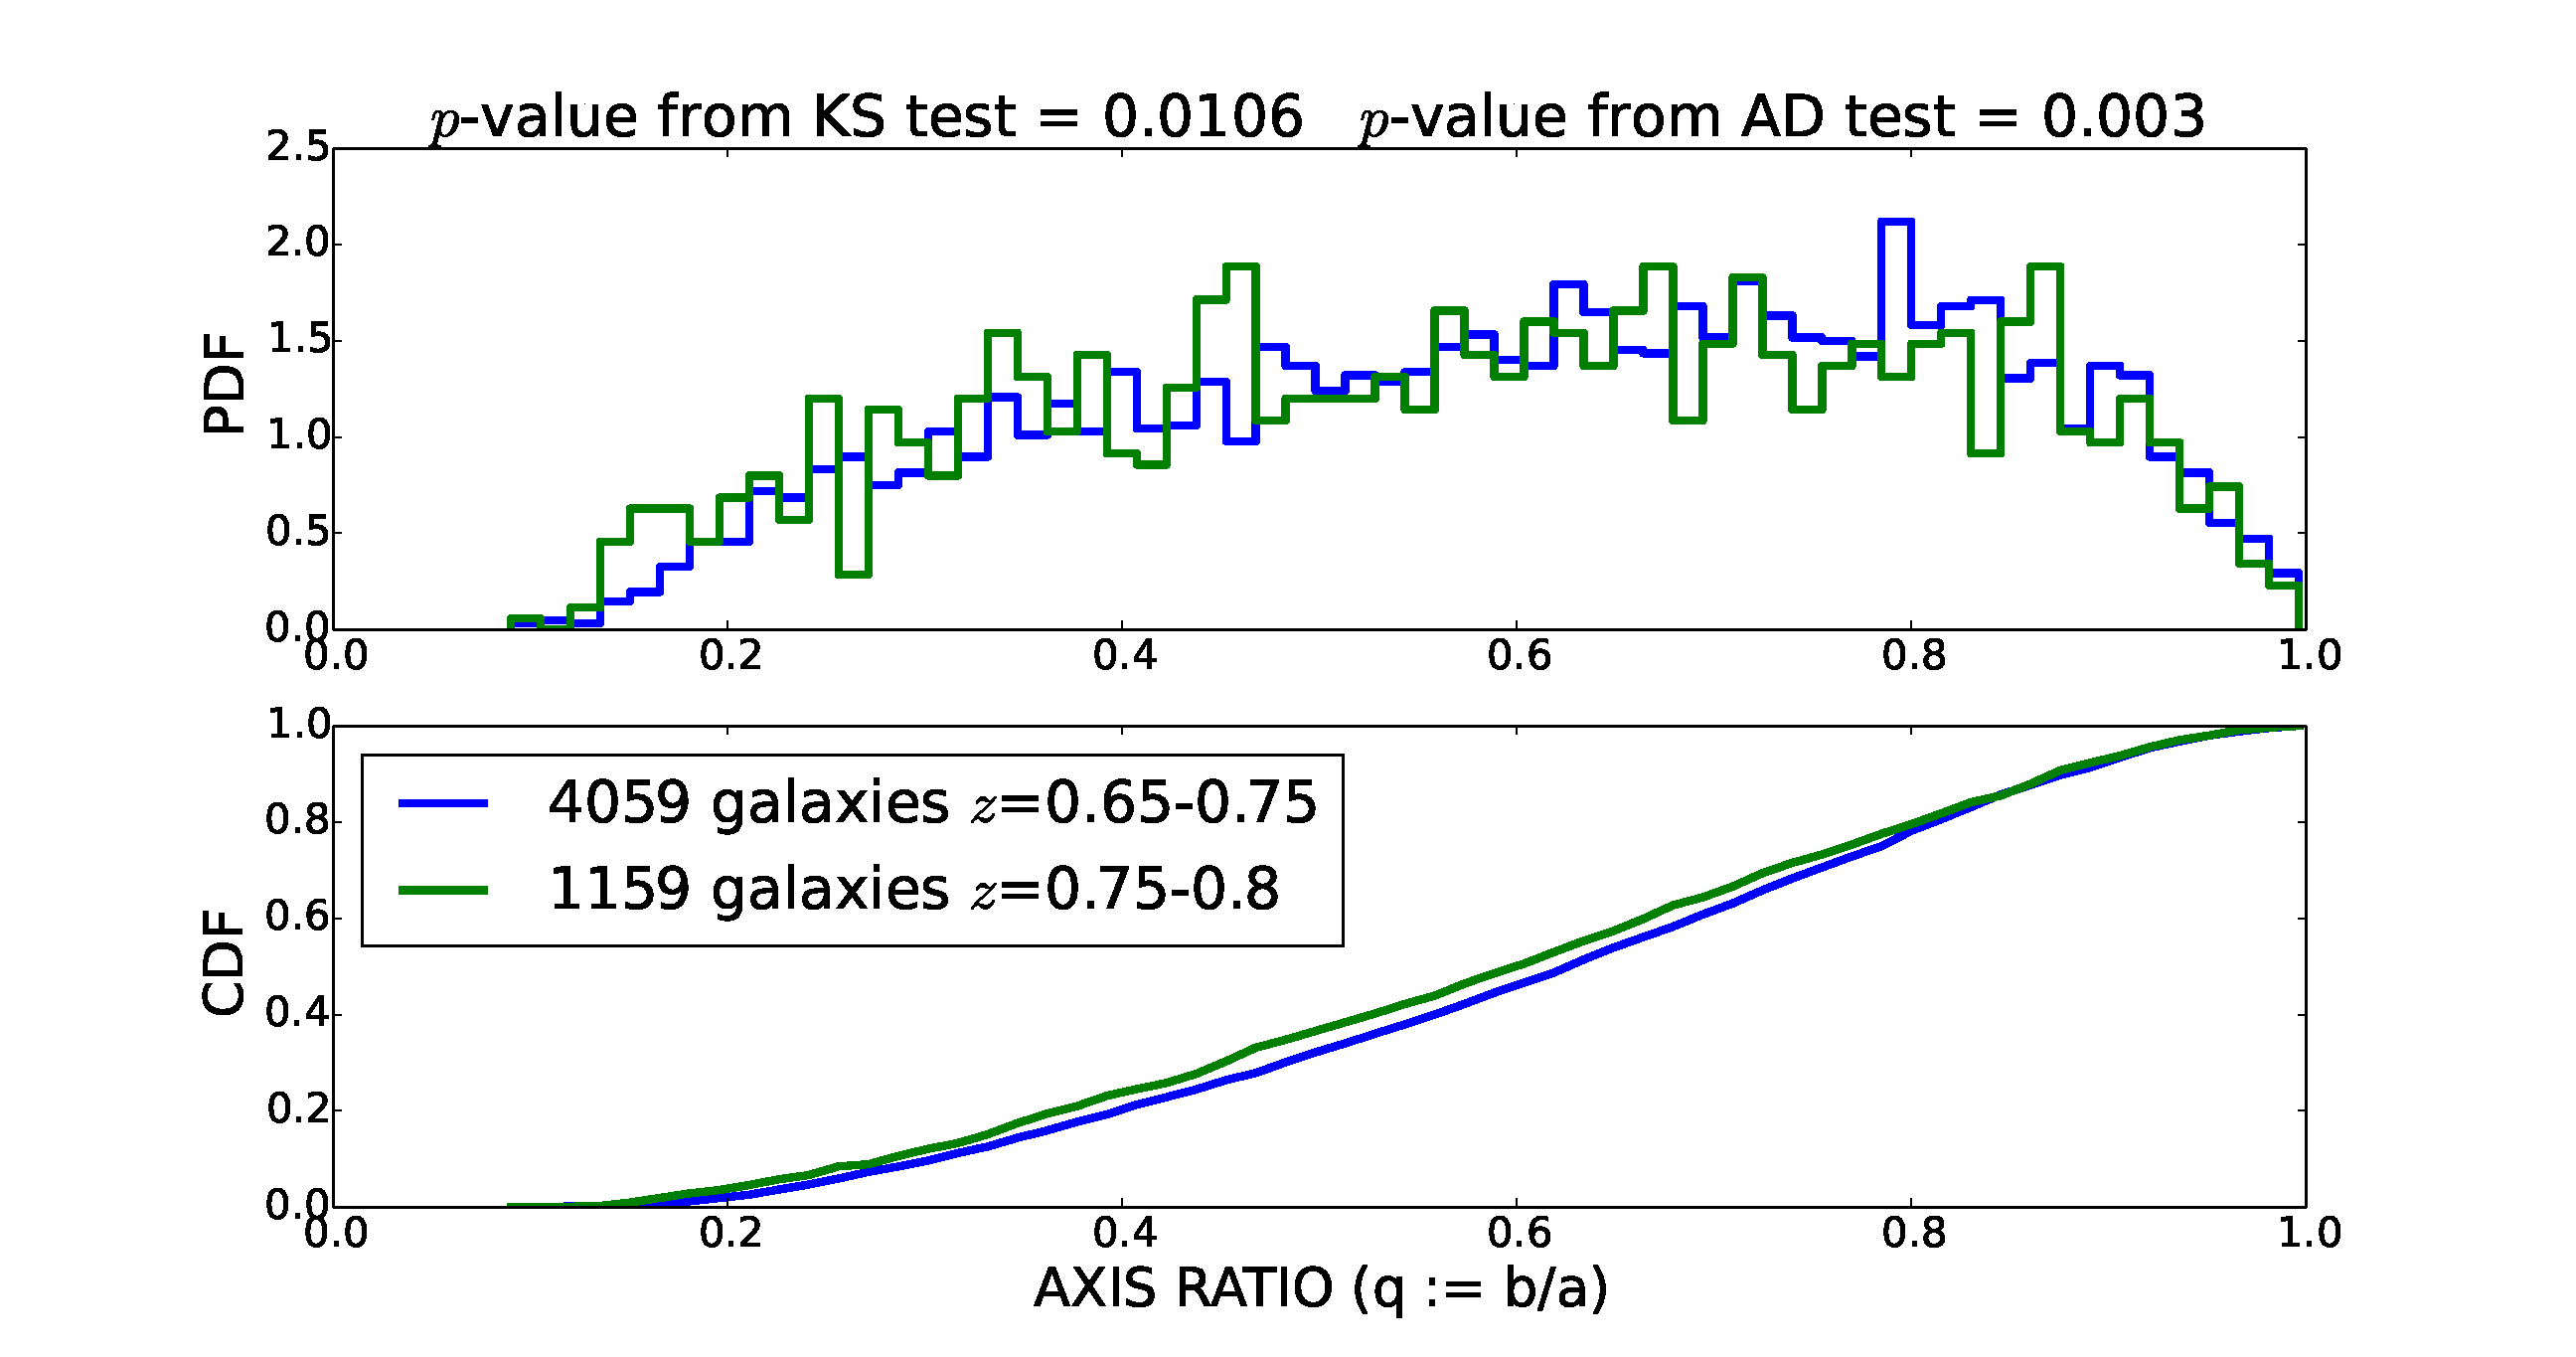
\includegraphics[width=0.9\columnwidth]{axisratio(0)_0dot65-0dot75_0dot75-0dot80.eps} \
 \caption{Comparison in contrasting environments: Axis ratios of galaxies in an underdense redshift bin, $z=0.55-0.65$ are compared with those in an overdense bin, $z=0.65-0.75$. $p$-values from the KS and AD test are given in Table.~\ref{table:pvalues_all}}
 \label{fig:axisratio_contrasting}
\end{figure*}

\begin{table}
 \centering
 \begin{tabular}[\columnwidth]{ | l | l | l | l | }
  \hline
  %\parbox[t]{0.15\columnwidth}{Redshift bins} & \parbox[t]{0.15\columnwidth}{Tests} & \parbox[t]{0.15\columnwidth}{Luminosity-selected} & \parbox[t]{0.15\columnwidth}{Luminosity-selected with B-band evolution} & \parbox[t]{0.15\columnwidth}{Stellar-mass-selected} \\
  Redshift bins & \s$1$ & \s$2$ & \s$3$ \\
  \hline
  All overdense vs.  & \scinot{1.1}{-4} & \scinot{2.6}{-5} & \scinot{1.9}{-6} \\
  All underdense     & \scinot{1}{-5} & $<\scinot{1}{-5}$ & $<\scinot{1}{-5}$ \\ \hline 
  $z:[0.65,0.75]$ (OD) vs. & 0.613 & 0.431 & 0.231 \\
  $z:[0.80,0.85]$ (OD) & 0.494 & 0.237 & 0.130 \\ \hline
  $z:[0.65,0.75]$ (OD) vs. & \scinot{5.8}{-4} & \scinot{1.5}{-5} & \scinot{3.5}{-6} \\
  $z:[0.55,0.65]$ (UD) & \scinot{9.8}{-4} & $<\scinot{1}{-5}$ & $<\scinot{1}{-5}$ \\ \hline
 \end{tabular}
 \caption{$p$-values from the Kolmogorov-Smirnov (top) and Anderson-Darling (bottom) obtained by comparing the distributions of axis ratios are given for three cases: \emph{all} overdense (OD) vs. \emph{all} underdense (UD), two overdense bins, not very separated in redshift and a pair of adjacent overdense and underdense bins. \s$1$, \s$2$, \s$3$ refer to the volume-limited sample in three different ways.
          The Anderson-Darling $p$-values are correct only upto 5 decimal places. 
% \rachel{What are the 0 entries in this and other tables?  Just how close to zero are they?  Since 0 is not really achieve, I recommend defining a value (such as $10^{-10}$ below which you will just say $<10^{-10}$ and give the value if it's above that, even if it seems really small to you, like $10^{-8}$.  Also, say $1.1\times 10^{-4}$ rather than $1.1e-4$.}
          }
 \label{table:pvalues_all}
\end{table}

\begin{table}
 \centering
 \begin{tabular}[\columnwidth]{ | l | l | l | l | }
  \hline
  %\parbox[t]{0.15\columnwidth}{Redshift bins} & \parbox[t]{0.15\columnwidth}{Tests} & \parbox[t]{0.15\columnwidth}{Luminosity-selected} & \parbox[t]{0.15\columnwidth}{Luminosity-selected with B-band evolution} & \parbox[t]{0.15\columnwidth}{Stellar-mass-selected} \\
  Redshift bins & \s$1$ & \s$2$ & \s$3$ \\
  \hline
  All overdense vs. & \scinot{5.6}{-4} & \scinot{1.0}{-4} & \scinot{3.3}{-6} \\
  All underdense    & \scinot{3}{-5} & \scinot{1}{-5} & $<\scinot{1}{-5}$ \\ \hline 
  $z:[0.65,0.75]$ (OD) vs. & 0.9563 & 0.7476 & 0.5359 \\
  $z:[0.80,0.85]$ (OD) & 0.5162 & 0.3352 & 0.2290 \\ \hline
  $z:[0.65,0.75]$ (OD) vs & \scinot{6.0}{-3} & \scinot{2.5}{-4} & \scinot{2.4}{4} \\
  $z:[0.55,0.65]$ (UD) & \scinot{1.2}{-2} & \scinot{2.5}{-4} & \scinot{5}{-5} \\ \hline
 \end{tabular}
 \caption{$p$-values from the Kolmogorov-Smirnov (top) and Anderson-Darling (bottom) obtained by comparing the ellipticities computed using second moments are given for three cases: \emph{all} overdense (OD) vs. \emph{all} underdense (UD), two overdense bins, not very separated in redshift and a pair of adjacent overdense and underdense bins. \s$1$, \s$2$, \s$3$ refer to the volume-limited sample in three different ways.  \arun{Should I write only two significant digits for higher $p$-values?}
           The Anderson-Darling $p$-values are correct only upto 5 decimal places. }
 \label{table:pvalues_momentbased_all}
\end{table}

%The distribution of the axis ratios that are obtained by the above manner are compared between redshift bins. 
We use two statistical tests namely the Kolmogorov-Smirnov test and Anderson-Darling test to compare distributions.
The Anderson-Darling test is carried out using the \texttt{adk} package\footnote{\url{http://www.inside-r.org/packages/cran/adk/docs/adk.test}} in \texttt{R}.

We first compare the distribution of the axis ratio in \emph{all}
overdense bins and \emph{all} underdense bins in Fig.~\ref{fig:axisratio_all}.
\rachel{How was the volume-limiting carried out for this?  You should say the answer to this question  for all figures.} 
\arun{The caption mentions it.}
\rachel{I'm afraid that's not enough.  Some people are going to read linearly and you want the info in the main text, too.}
Unless otherwise mentioned, the axis ratios refer to the values obtained using the method of \cite{Claire_Fits}.
The cumulative distinction functions are also plotted alongside in order to be able to visualize the `distance' between the distributions.
Referring to the first two rows in Table~\ref{table:pvalues_all}, we see that the p-values from both the KS and AD tests are well below 0.05, 
so we reject the `null hypothesis' that the overdense and underdense regions have same axis ratio distributions at 95\% significance level.

One might imagine that the disagreement between the distributions is, at least partly, due to the fact that the overdense and underdense sample have different redshift distributions.
To show that that is not the case, we will compare distributions between two overdense / underdense redshift bins, where we expect to find similarity, and between an overdense and underdense regions,
where we expect the distributions to differ.
Figures~\ref{fig:axisratio_similar} and~\ref{fig:axisratio_contrasting} are examples showing that the distributions are indeed similar when the environments are similar and different when the environments are different, confirming our expectation.
Similar conclusion can be arrived at by comparing other redshift bins.

Such a trend is also observed in axis ratios based on second moments. 
If $Q_{ij}$ represents the generic matrix element of the matrix of second moments, then define a complex number, sometimes known as the \emph{distortion}, as
\begin{equation}
 e = e_1 + ie_2 = \frac{Q_{11}-Q_{22}+2iQ_{12}}{Q_{11}+Q_{22}}.
 \label{eq:distortion}
\end{equation}
%\arun{Is this the correct denominator?} \rachel{Yes.  There's another ellipticity definition with a different denominator, but we use distortion which is defined as in this equation.  (Once you read this response feel free to delete this conversation.)}
Then, one definition of ellipticity is the magnitude of this complex number which is $\sqrt{e_1^2+e_2^2}$.

After neglecting a small fraction $(\sim 0.0065\%)$ of galaxies (36 out of 55991 galaxies between $0.3\le z<0.85$ with $\log(M/\Msun) > 10.15$) for which the moments do not converge, 
we make comparisons to the above between the distribution of ellipticities computed from the second moments and the results are tabulated in Table~\ref{table:pvalues_momentbased_all}.
Once again, we see that the distributions are consistent with each other when the environment is similar and are inconsistent when the environments are constrasting.

\subsubsection{RMS ellipticites}
\begin{figure}
 %\centering
 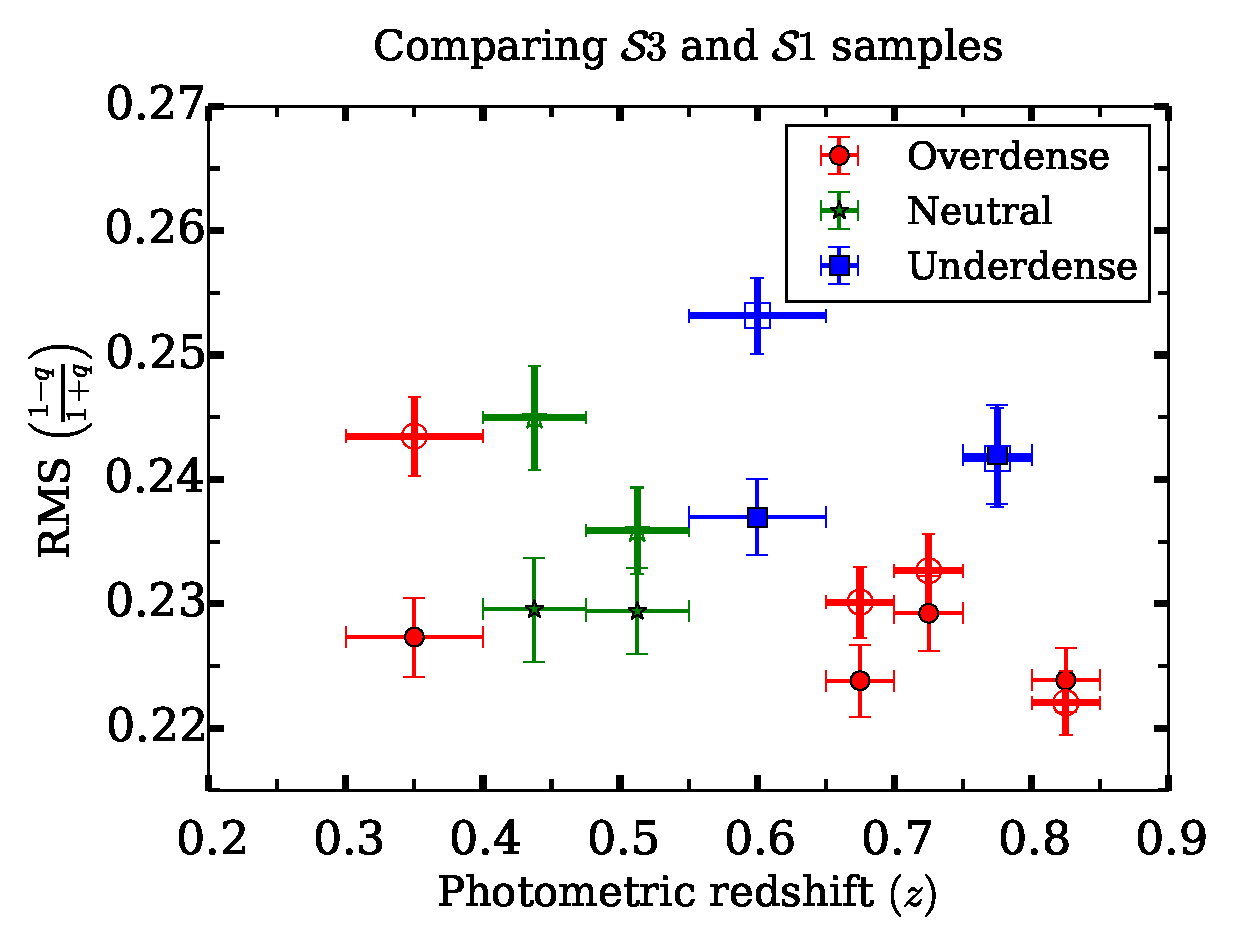
\includegraphics[width=1.0\columnwidth]{rms_ellip1_noevolution.eps} \
 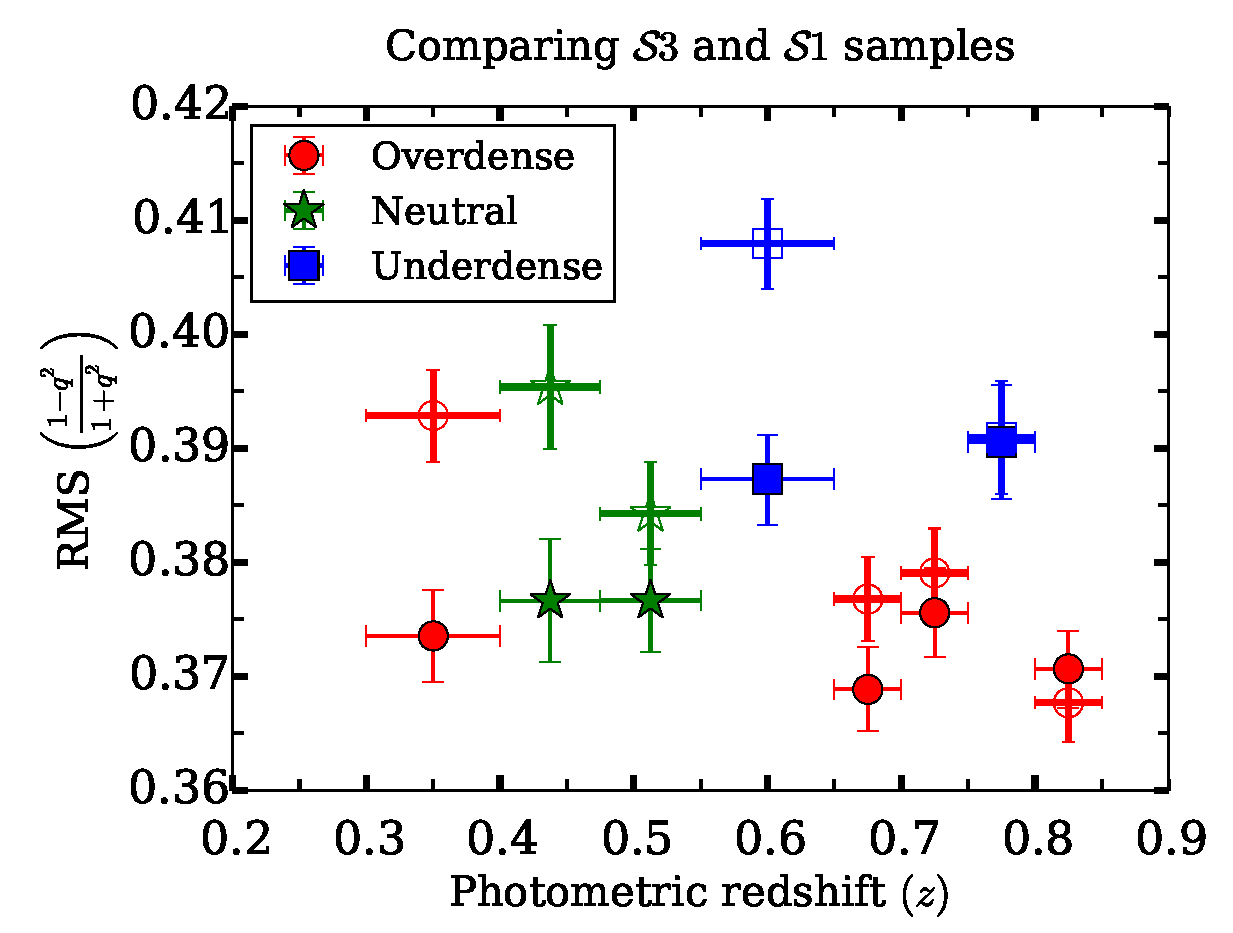
\includegraphics[width=1.0\columnwidth]{rms_ellip2_noevolution.eps} \\
 \caption{Left: RMS ellipticities with ellipticity defined as $\frac{1-q}{1+q}$. \; 
          Right: RMS ellipticities with ellipticity defined as $\frac{1-q^2}{1+q^2}$.\\ The horizontal errorbars simply correspond to the binwidth while the vertical ones
          are $1\sigma$ errorbars obtained by bootstrapping. \rachel{I'm thinking these are so similar we just need to show one figure, and can say the results for the other in words.  The same goes for the next figure.}}
 \label{fig:rms_ellip}
\end{figure}

\begin{figure}
 %\centering
  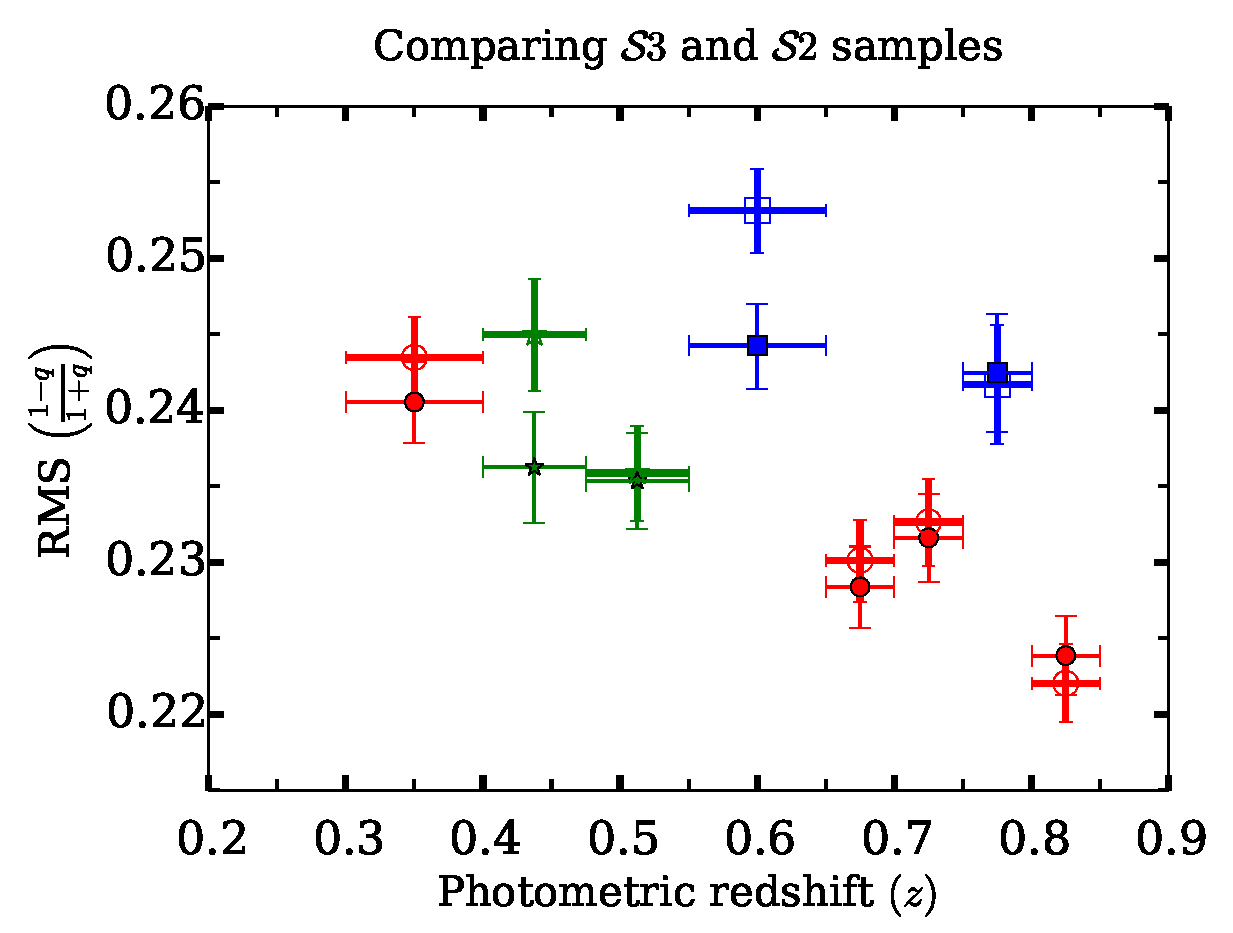
\includegraphics[width=1.0\columnwidth]{rms_ellip1_Bbandevolution.eps} \
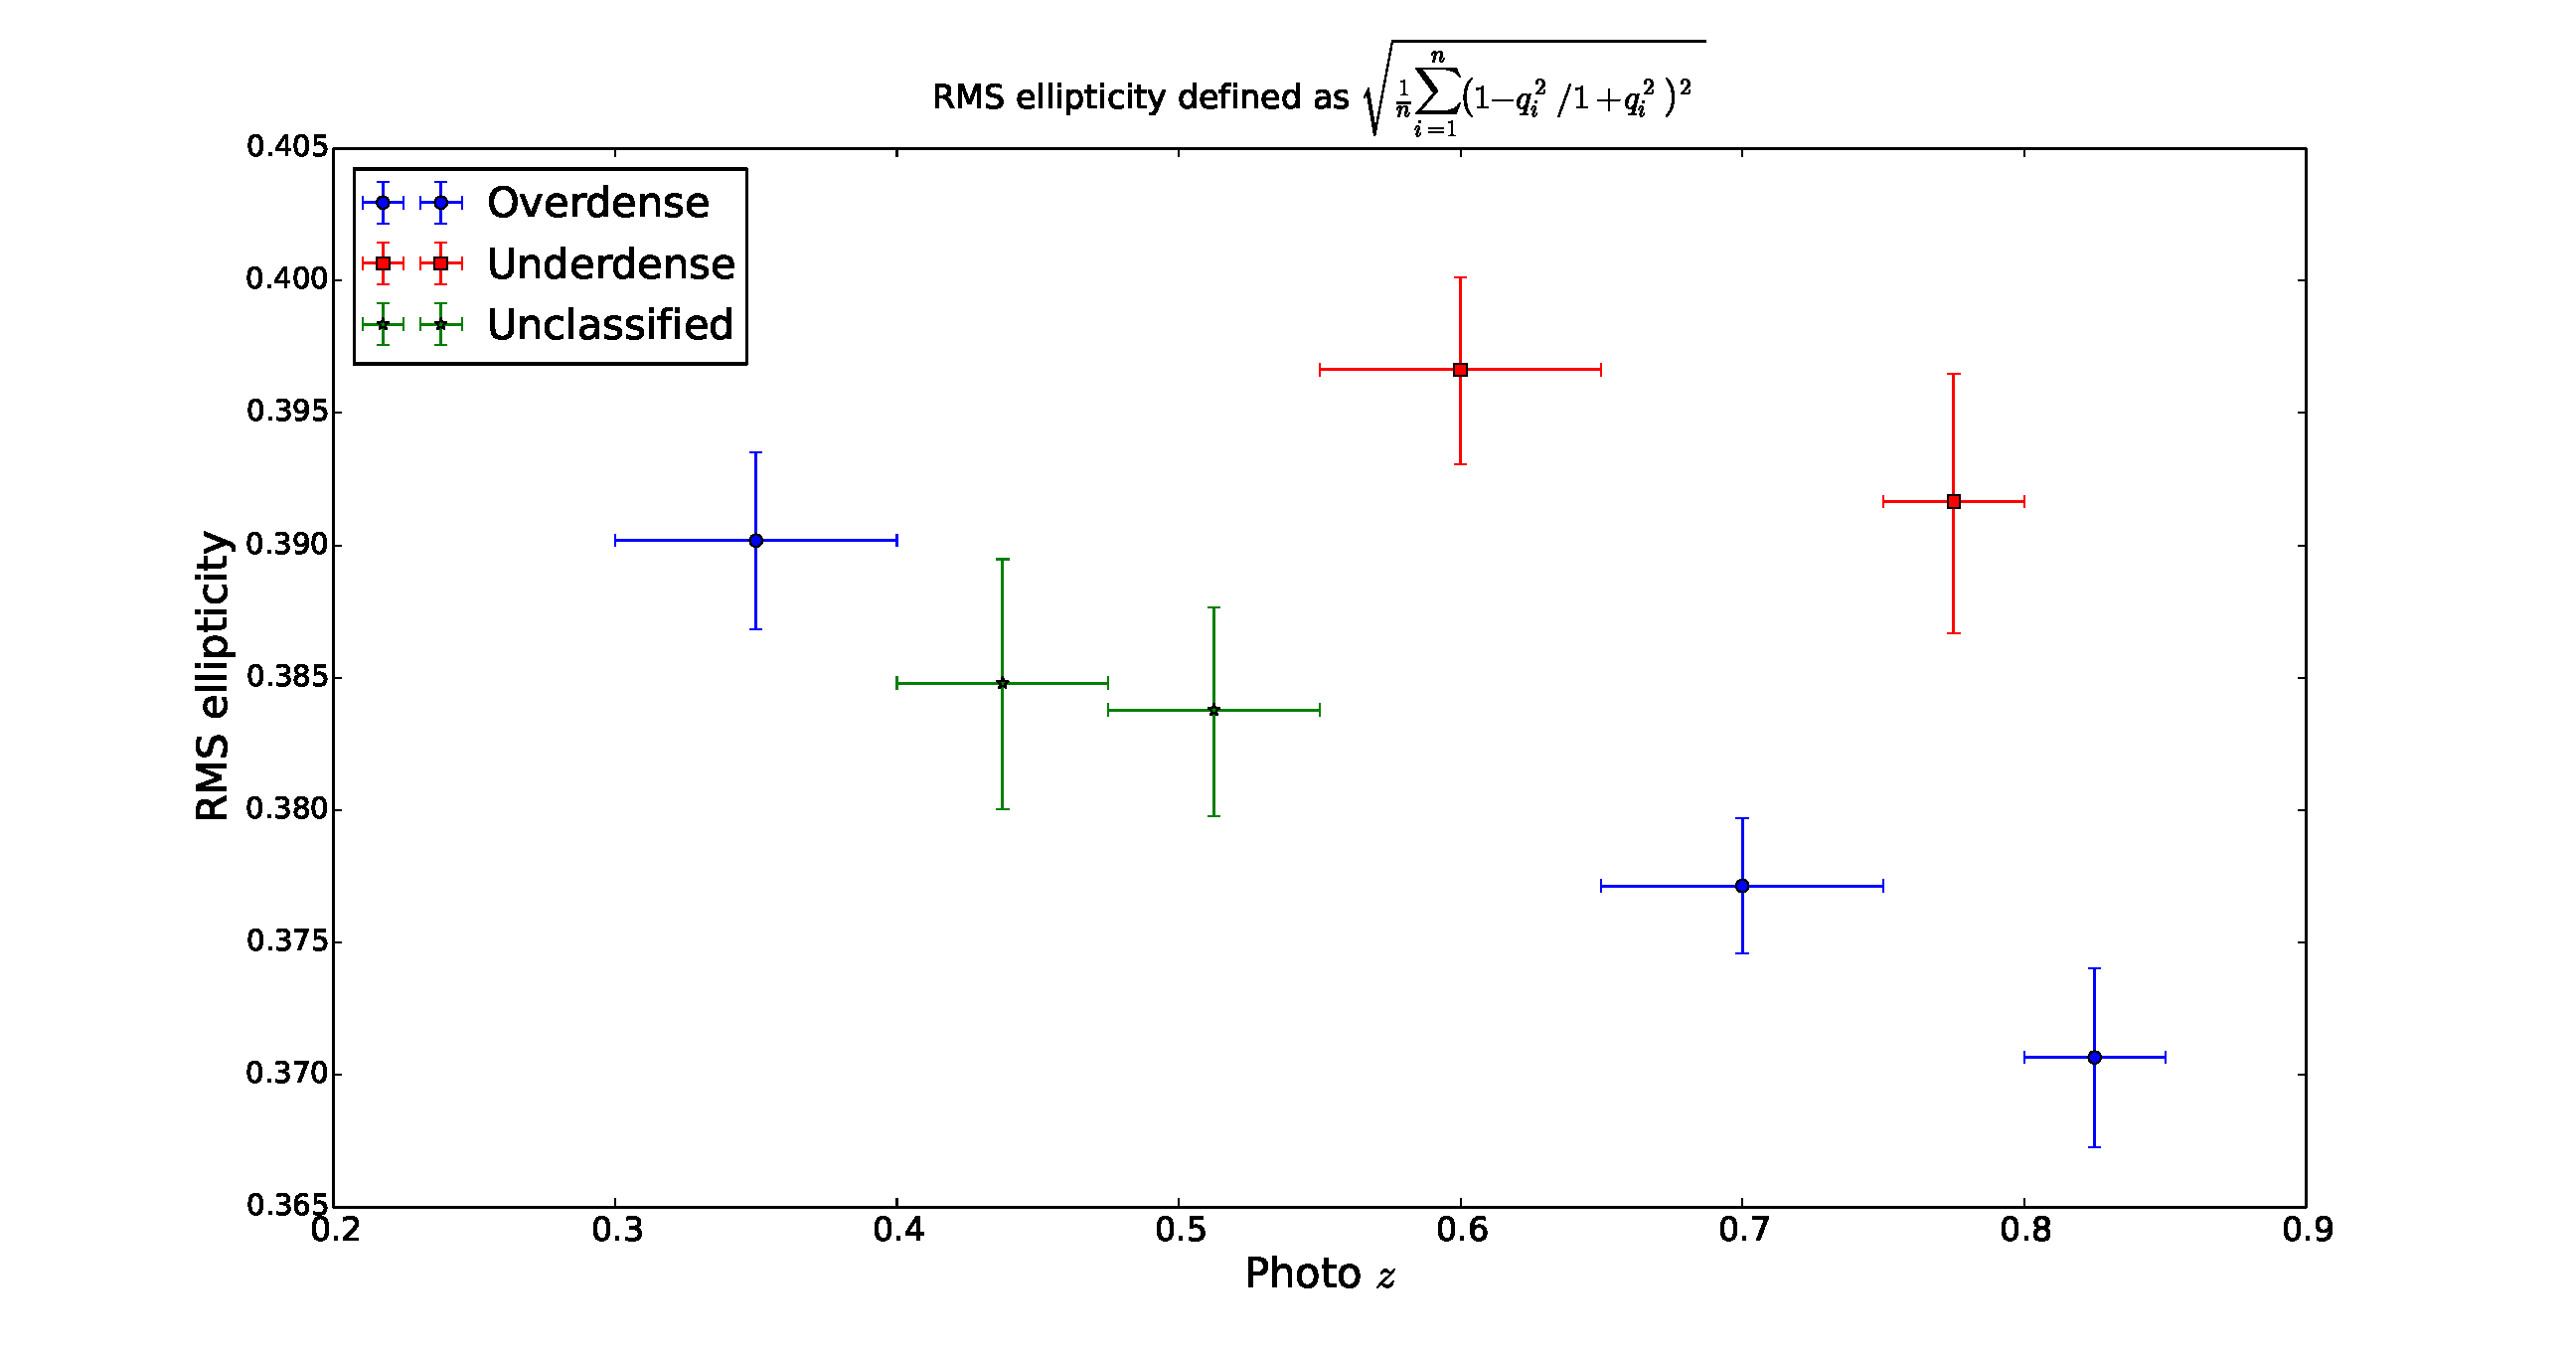
\includegraphics[width=1.0\columnwidth]{rms_ellip2_Bbandevolution.eps} \\
 \caption{Left: RMS ellipticities with ellipticity defined as $\frac{1-q}{1+q}$. \; 
          Right: RMS ellipticities with ellipticity defined as $\frac{1-q^2}{1+q^2}$.\\ The horizontal errorbars simply correspond to the binwidth while the vertical ones
          are $1\sigma$ errorbars obtained by bootstrapping. The solid points correspond to the sample where the luminosity cut evolves by -1.23 per unit redshift (\s$2$) and the unfilled
          points correspond to the sample obtained from stellar mass cuts (\s$3$).}
 \label{fig:rms_ellip_Bband_mass}
\end{figure}

\begin{figure}
 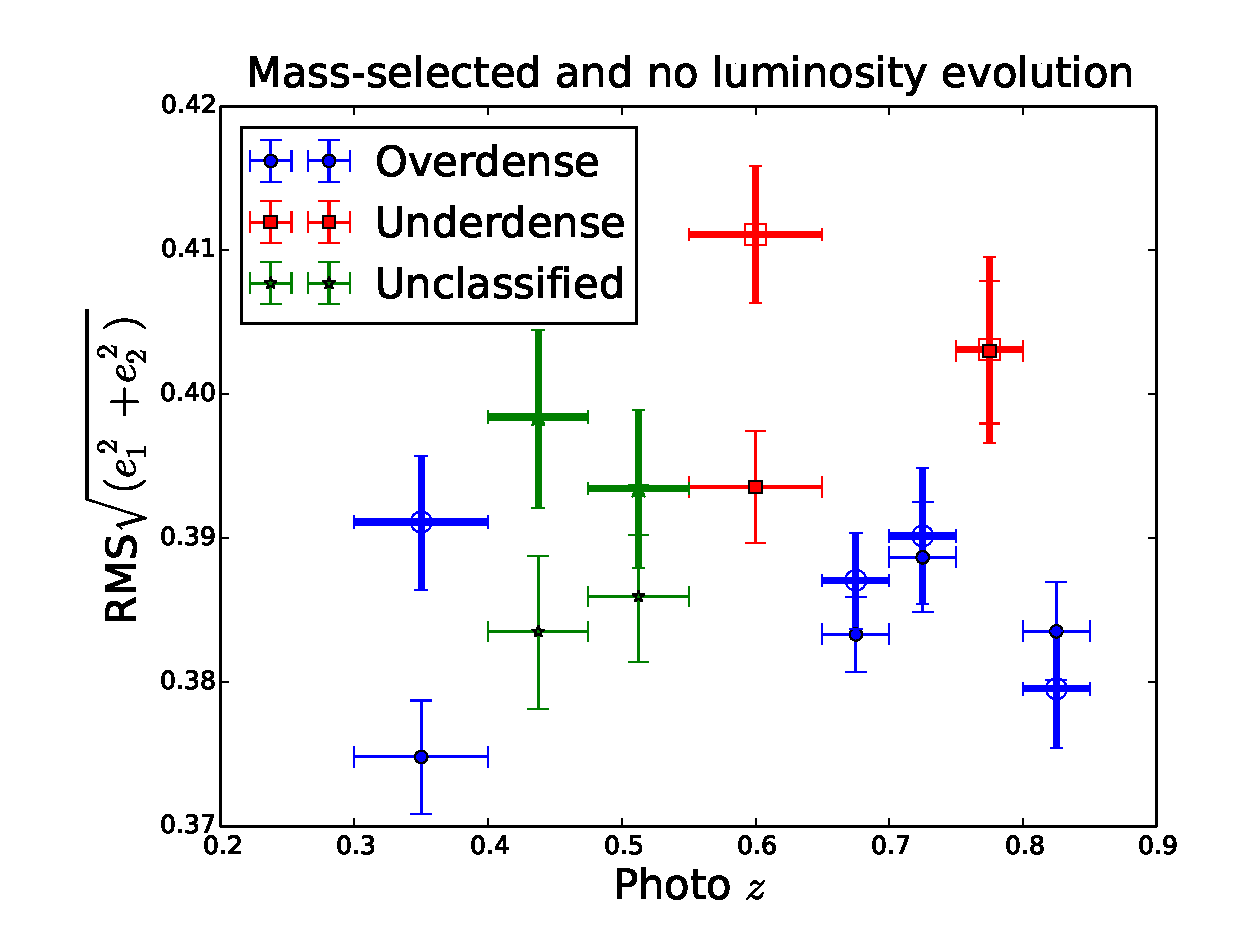
\includegraphics[width=1.0\columnwidth]{rms_ellip_momentbased_noevolution.eps} \
 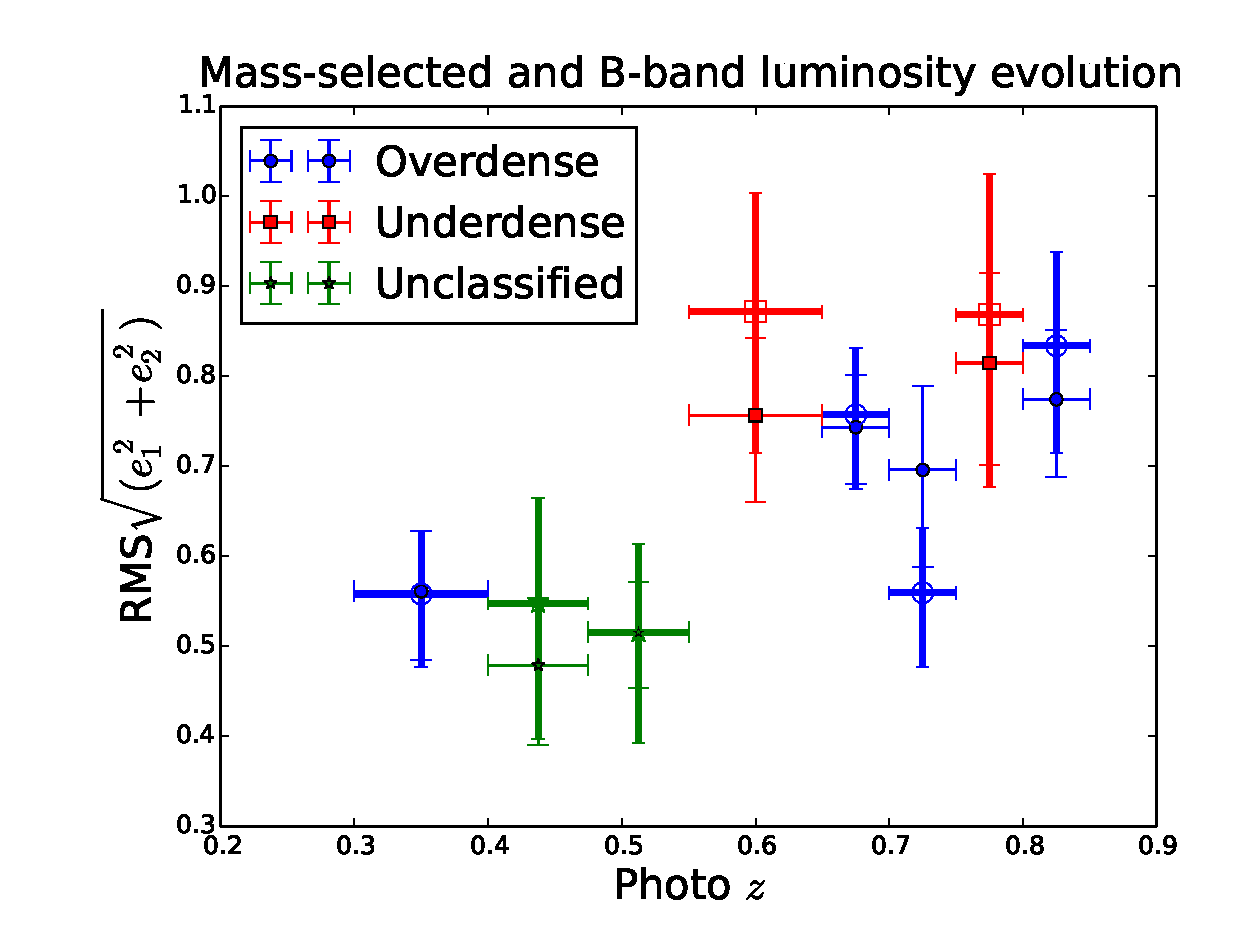
\includegraphics[width=1.0\columnwidth]{rms_ellip_momentbased_Bbandevolution_masscut.eps} \\
 \caption{RMS ellipticies with ellipticity defined as $\sqrt{e_1^2+e_2^2}$, where $e_1$ and $e_2$ are the real and imaginary components of the distortion defined in Eq.~\ref{eq:distortion}.
          The horizontal errorbars simply correspond to the binwidth while the vertical ones
          are $1\sigma$ errorbars obtained by bootstrapping. The solid points correspond to the luminosity selected sample (\s$1$ sample on the left and \s$2$ sample on the right) and the unfilled
          points correspond to the sample obtained from stellar mass cuts (\s$3$). }
 \label{fig:rms_ellip_momentbased}         
\end{figure}


%The shape of a population of galaxies can be characterized by a single number called `RMS ellipticity'. If $q=b/a$ is the axis-ratio, then the ellipticity maybe defined as $\frac{1-q}{1+q}$
%or as $\frac{1-q^2}{1+q^2}$. The root mean squared (RMS) of ellipticities of galaxies in each redshift bin are shown in Figure~\ref{fig:rms_ellip}.
For the luminosity-selected sample without any evolution, RMS ellipticities of galaxies in each redshift bin are shown in Figure~\ref{fig:rms_ellip}. As one can see, the underdense regions
have significantly higher values for RMS ellipticities when compared to the overdense regions. Note in particular that we've been able to capture the narrow overdense bin $0.75\le z < 0.80$.  
There is (almost) no redshift dependence in the figure.

The dependence on the local environment seems to make sense. Overdense regions typically have young, spiral galaxies which have high $q$ and hence low RMS ellipticity. 
On the contrary, the underdense regions typically have old, elliptical galaxies and thus low $q$ and high RMS ellipticity.

From Figs.~\ref{fig:redshift_fluxlimited} and~\ref{fig:redshift_vollimited},
the region $0.4\le z < 0.55$ show signs of being marginally underdense but have low RMS ellipticities too that agree with the rest of the overdense regions.

When the B-band luminosity evolution is taken into account in selecting the sample, a systematic increase in the ellipticity at lower redshifts can be observed. We plot these alongside with stellar-mass selected samples, where a similar trend is found, in Fig.~\ref{fig:rms_ellip_Bband_mass}. 
Also, the RMS values of the ellipticites calculated from the second moments within each redshift bin are given in Fig.~\ref{fig:rms_ellip_momentbased}.

\subsection{Other morphological parameters}
For other morphological parameters such as the \sersic index and \btt ratio, we do not compare the distributions themselves directly. 
For \sersic profile fits, it gets tricky since we truncate the \sersic index at 6. 
For \btt ratios, we force the value to be between 0.05 and 0.95. %\arun{What exactly do we do here?}.
We will understand the dependence of these quantities on environment by computing the median values in different redshift bins.
We choose median over mean since it is more robust to the truncation effects.
Fig.~\ref{fig:median_sersicn} show the median of the \sersic index with and without taking into account of the luminosity evolution. Median values obtained using stellar mass selected samples are plotted alongside for reference.
We observe that the overdense regions tend to have higher \sersic index than the adjacent underdense ones.
Fig. \ref{fig:median_dvcbtt} show the variation of median \btt ratio with redshift. We see that the bulge component is more in overdense regions than in the underdense regions.
These two observations are consistent with each other since higher \sersic index implies higher bulge component which are typical in young galaxies found in overdense regions.

In Fig.~\ref{fig:median_sersicn}, we see that the \sersic indices of mass selected sample (\s$3$) are systematically greater than those of the luminosity selected samples (\s$1$,\s$2$).
This is consistent with the \btt values being higher in \s$3$ than in \s$1$ or \s$2$ in Fig.~\ref{fig:median_dvcbtt}. This is not just an edge effect but can be seen from the distributions themselves 
that the mass selected sample doesn't include as many disk-like galaxies as in luminosity selected samples.
%We chose median over mean since \sersic n greater than 6 are truncated to 6. This affects the mean statistic more than the median.
\begin{figure}
 %\centering
 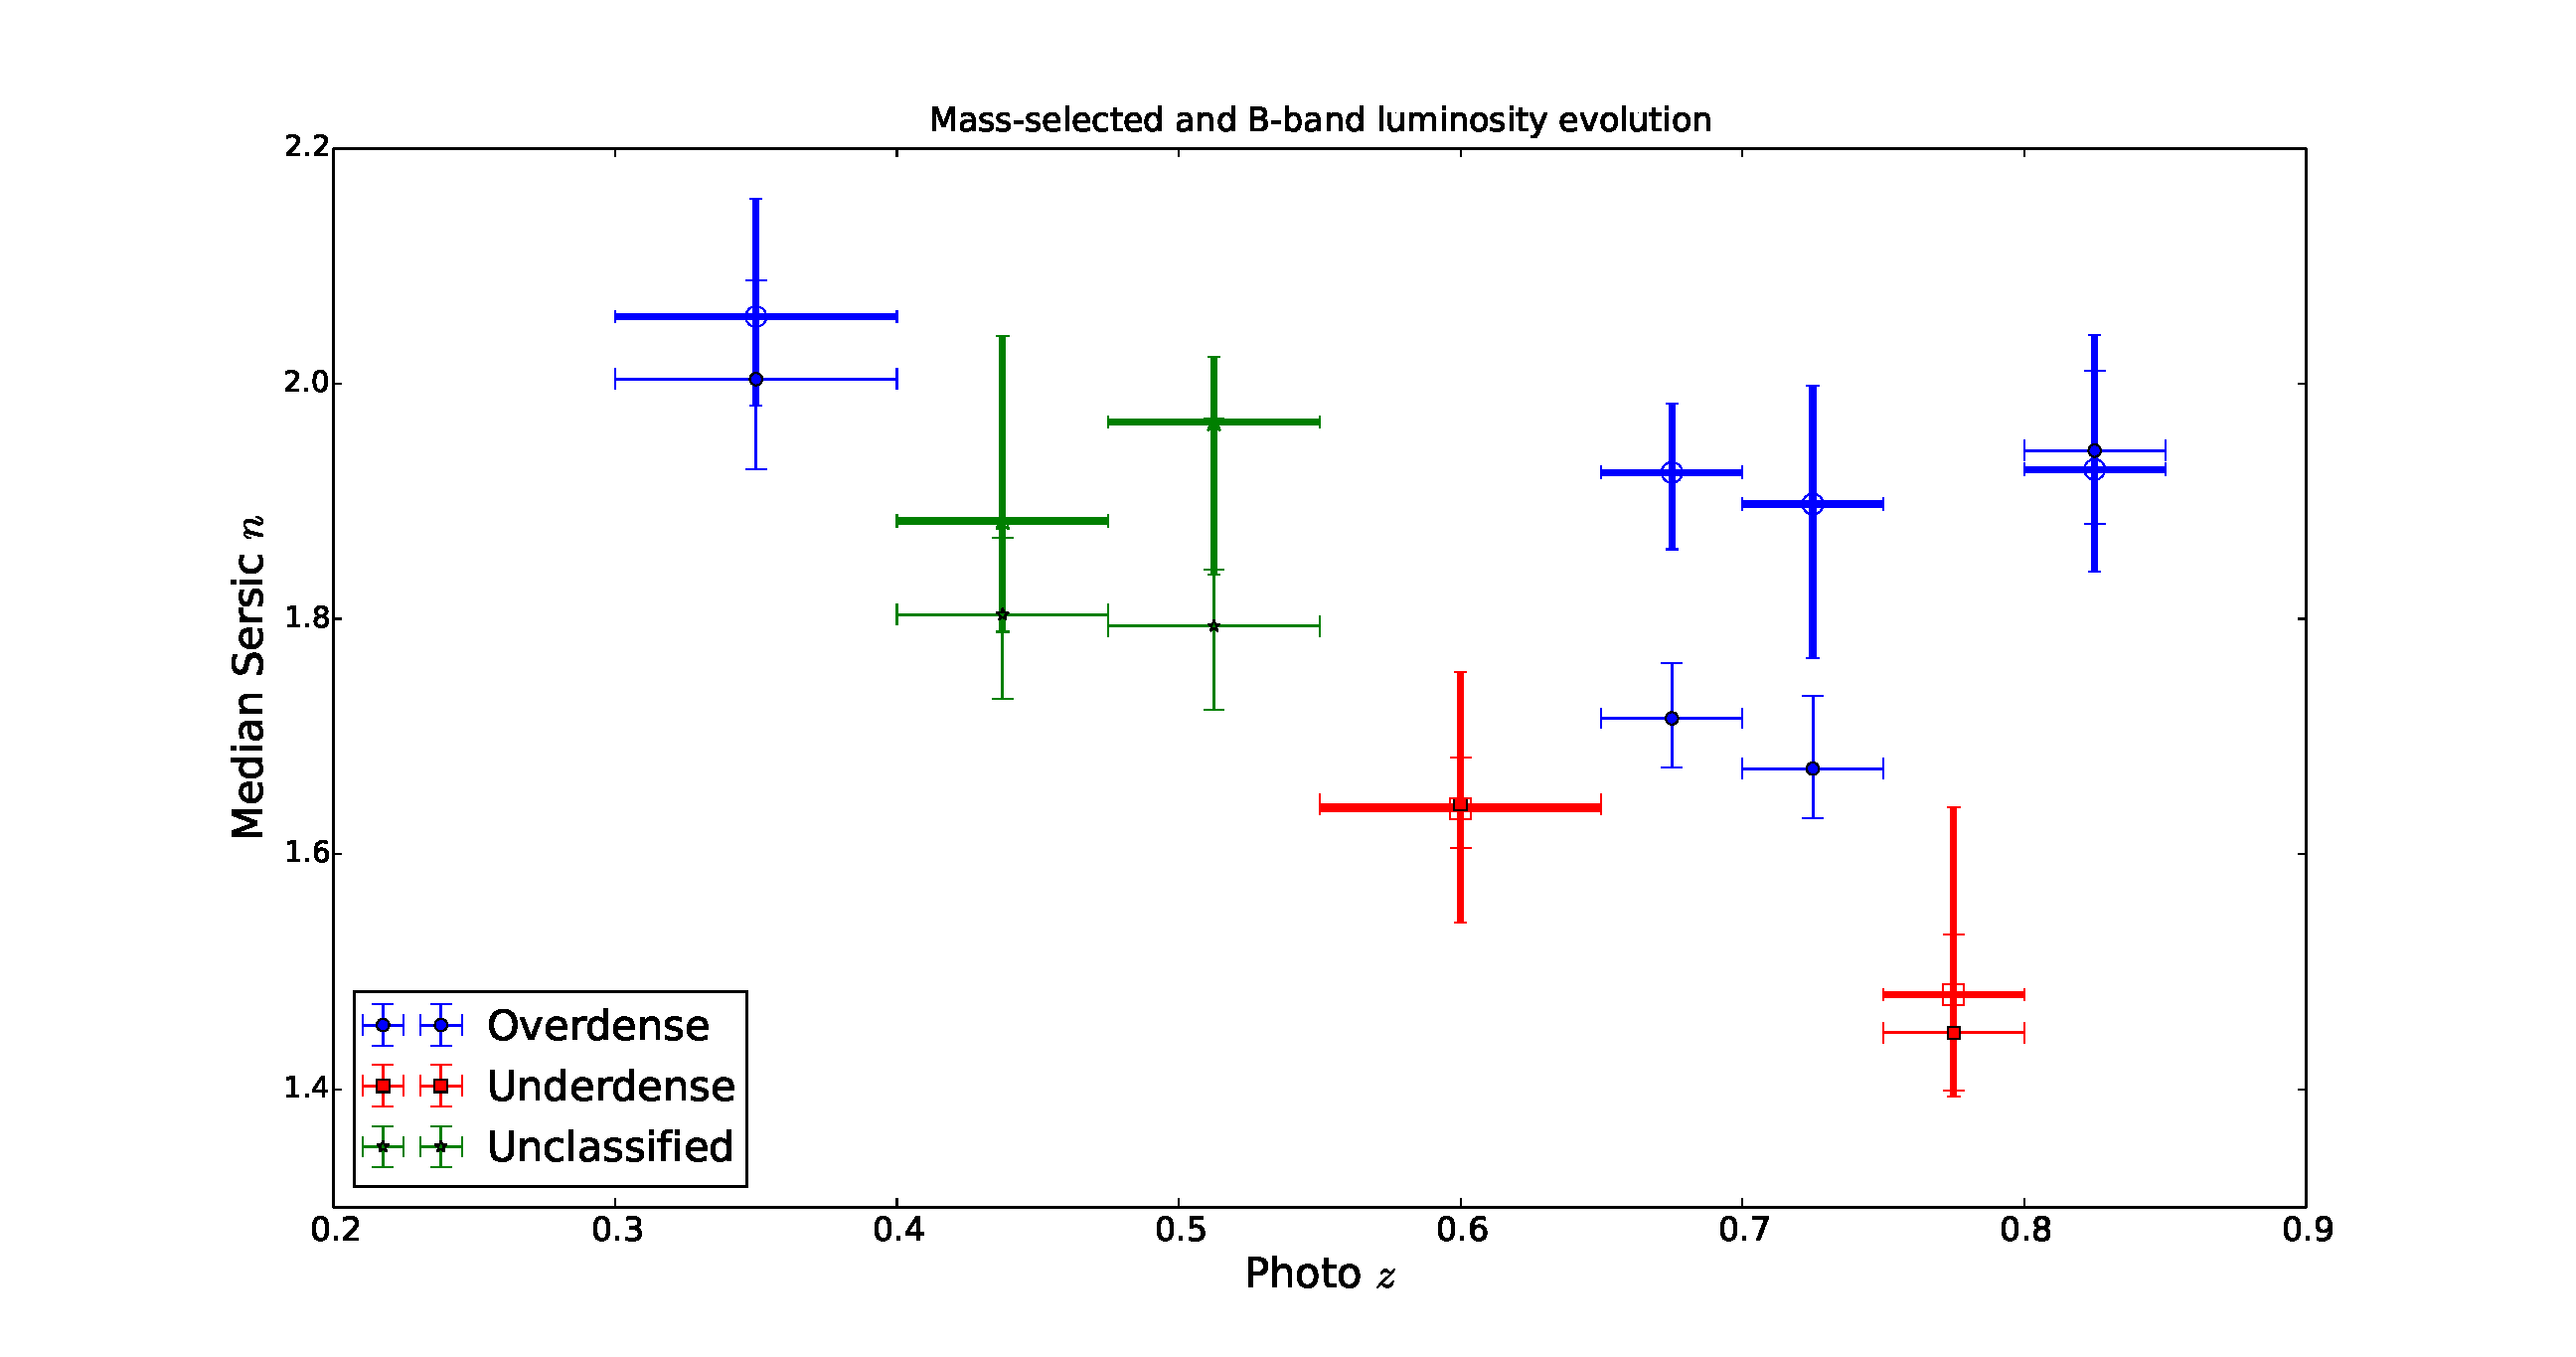
\includegraphics[width=1.0\columnwidth]{median_sersicn}
 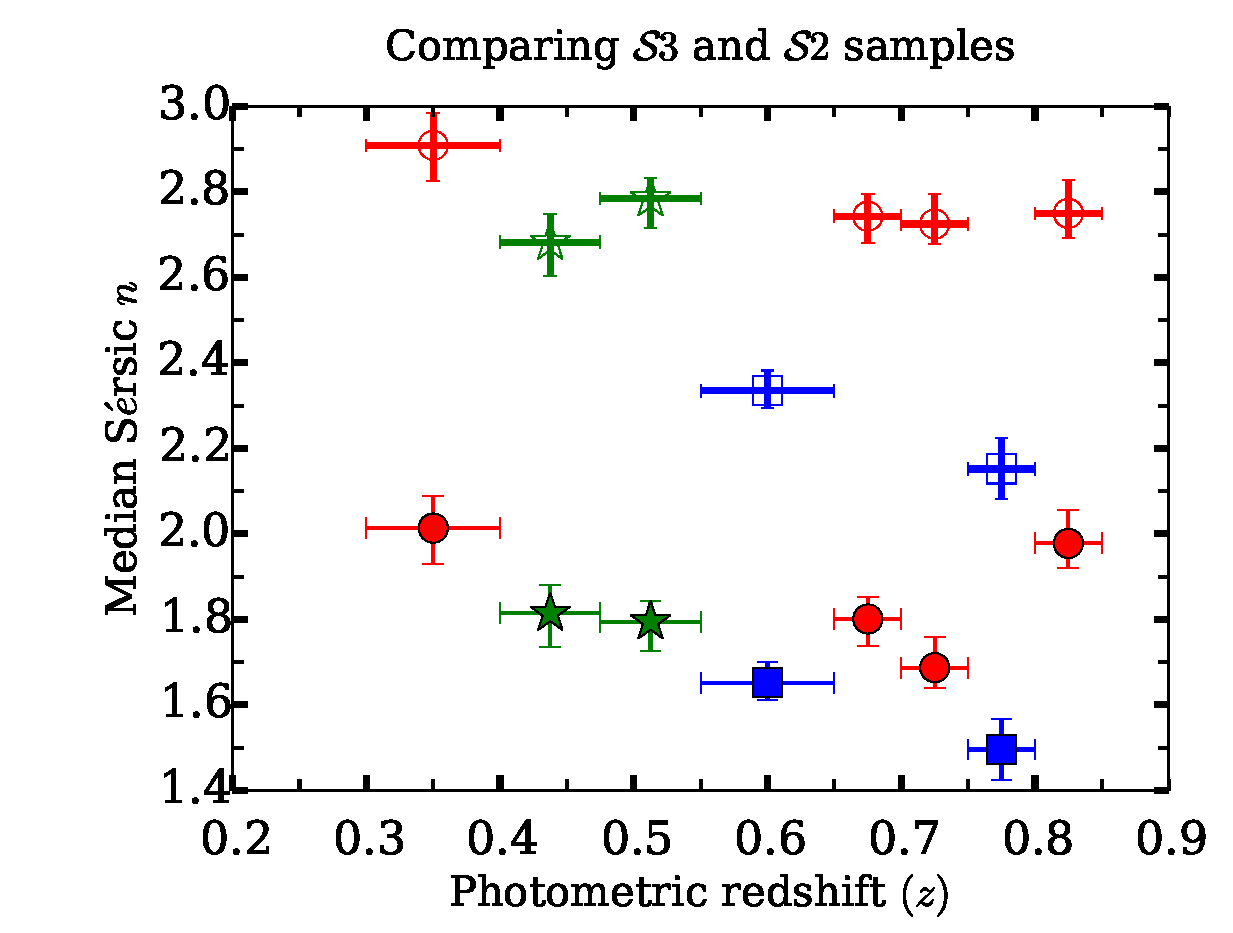
\includegraphics[width=1.0\columnwidth]{median_sersicn2}
 \caption{Median values of the \sersic indices for volume-limited samples \s$1$ and \s$3$ are plotted (filled centers and thin errorbars) in left and right panels respectively for each redshift bin.
          Median values for the \s$2$ sample are plotted in both the panels (open centers and thick errorbars) in both the panels.
          The horizontal errorbars simply correspond to the binwidth while the vertical ones are $1\sigma$ errorbars obtained by bootstrapping. \rachel{Only need to have a legend on one panel, since the legends on both panels are the same.  Same comment applies to next figure.}}
 \label{fig:median_sersicn}
\end{figure}

\begin{figure}
 %\centering
 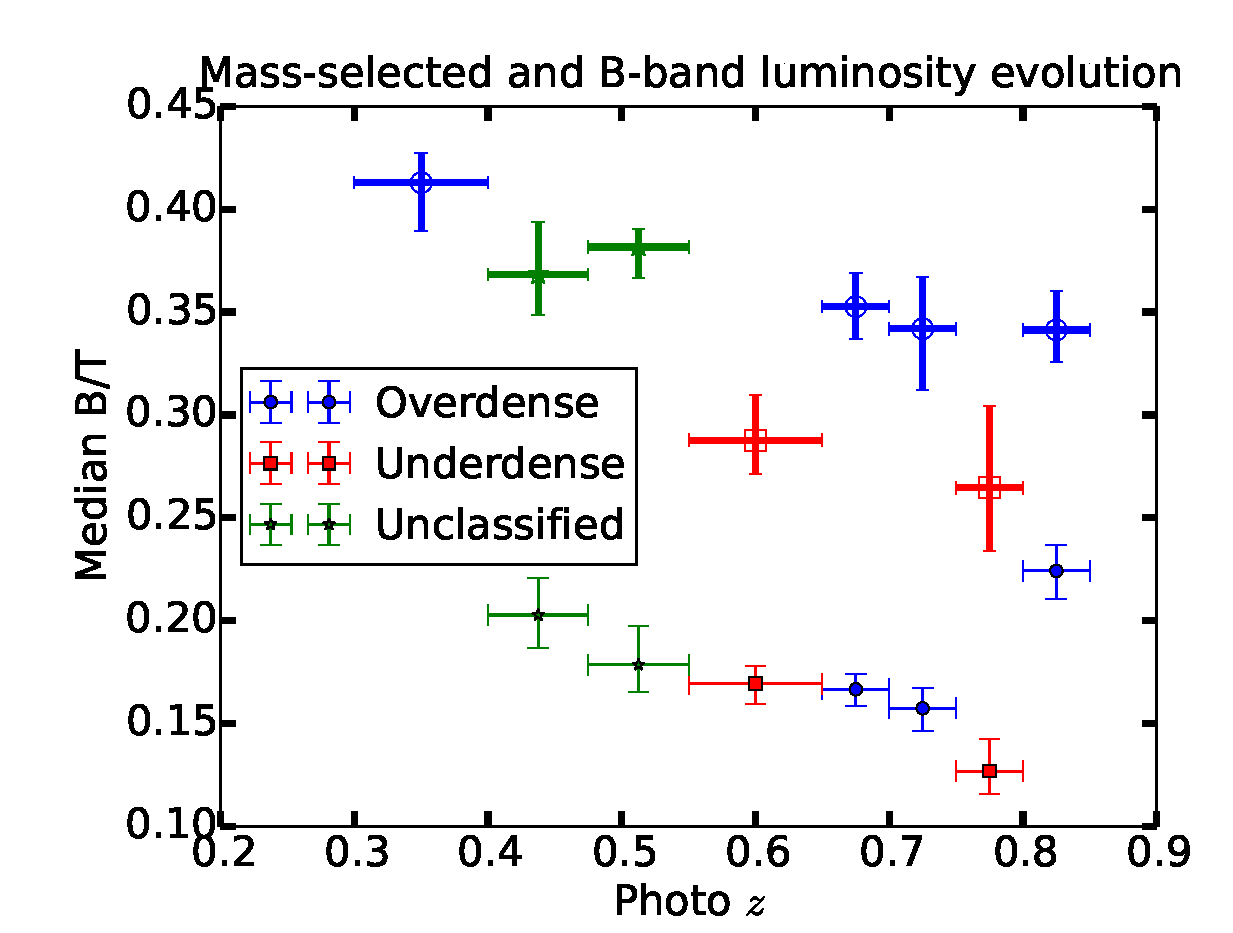
\includegraphics[width=1.0\columnwidth]{median_dvcbtt1}
 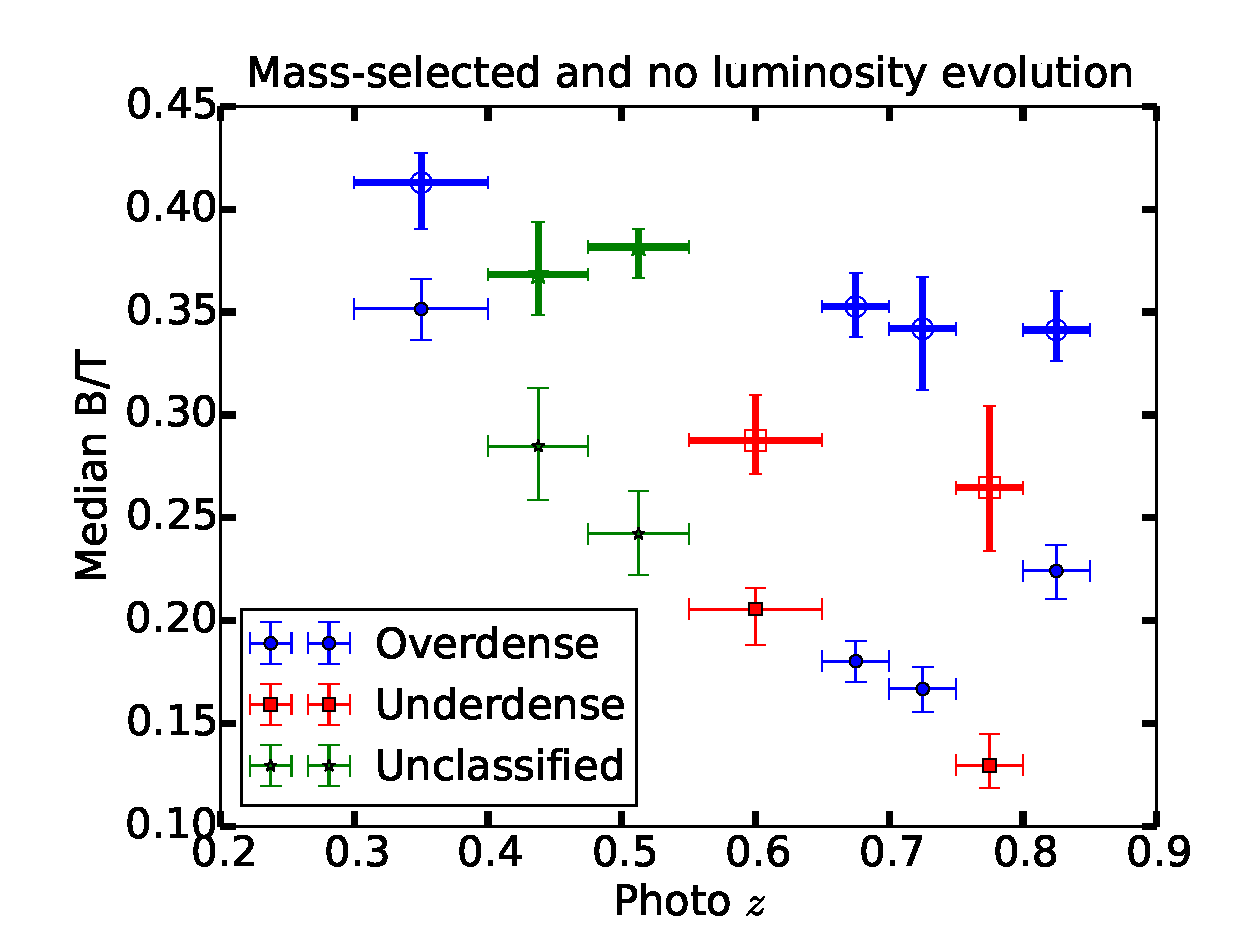
\includegraphics[width=1.0\columnwidth]{median_dvcbtt2}
  \caption{Median values of the \btt ratios for volume-limited samples \s$1$ and \s$3$ are plotted (filled centers and thin errorbars) in left and right panels respectively for each redshift bin.
          Median values for the \s$2$ sample are plotted in both the panels (open centers and thick errorbars) in both the panels.
          The horizontal errorbars simply correspond to the binwidth while the vertical ones are $1\sigma$ errorbars obtained by bootstrapping.  \rachel{These look so similar that I am questioning the need to have both.  Perhaps remove one and mention that they are nearly identical in the text.}}
 \label{fig:median_dvcbtt}
\end{figure}

\section{Conclusions}
\label{S:summary}

In this study, we have shown that morphological parameters of galaxies depend on the local environments along the line of sight in a manner than affect Weak Lensing simulations.
In studies of Weak Lensing, one simulates galaxy images in a redshift slice by learning from the images in the same redshift bin of a training sample like COSMOS, which we have used for our analysis here.
The survey volume is broken up into multiple redshift slices and are classified as `overdense', `underdense' or `neutral' according to their local environment.
This is done by comparing the 1-D redshift distribution to some of the parametric models available in the literature. 
The incompleteness in the sample is minimized by constructing a volume limited sample either by imposing stellar mass cuts (\s$3$) or by imposing a luminosity cut. 
Further, depending on whether we have the cut fixed or evolve with redshift, we get two more volume limited samples \s$1$ and \s$2$ respectively. 
Morphological parameters are obtained by fitting a single \sersic profile to the images or by a two component (bulge+disk) fit. 
The morphological quantities of interest include axis ratios or equivalently the ellipticities, \sersic indices and \btt ratios.

For all the three volume-limited samples, we compare the distributions of the axis-ratios of the galaxies in overdense and underdense regions and conclude that the distributions are different after performing statistical tests on them.
From the axis ratios, we compute ellipticities and find that the root mean squared value of the ellipticities of galaxies in a redshift bin vary significantly between the overdense and underdense regions.
Such a behavior is also observed when ellipticies are computed using second moments instead of a parametric model fitting. \sersic index and \btt ratios also exhibit similar trends
with redshift based on the local environment. 

Our result has serious implications for realistic image simulations for Weak Lensing. 
It suggests that the training sample is affected by cosmic variance so as to possibly bias the conclusions from the simulations. 
This is particularly a problem with narrow surveys where a single galaxy cluster or a void could affect the environment significantly. 
Thus, we are forced to use wider redshift bins, much larger than the uncertainties in the redshifts, so as to be able to wash out the environmental dependence.
However, future surveys such as the Large Synoptic Survey Telescope\citep[LSST;][]{LSST_Book} will image larger areas of sky mitigating the dependence of local environment in image simulations.

\section*{Acknowledgments}

AK and RM acknowledge the support of NASA ROSES 12-EUCLID12-0004, and
program HST-AR-12857.01-A, provided by NASA through a grant from the
Space Telescope Science Institute, which is operated by the
Association of Universities for Research in Astronomy, Incorporated,
under NASA contract NAS5-26555. RM acknowledges the support of an Alfred P. Sloan Research Fellowship.  We thank Alexie Leauthaud for 
many useful discussions.


%\begin{thebibliography}
\bibliography{ref}
%\end{thebibliography}
\end{document}


